\documentclass[11pt,a4paper,twoside]{book} %scrbook book report
\usepackage{hyperref}  % Necesario para manejar los enlaces
\usepackage[
backend=biber,
style=apa,
%sorting=none,
backref=true,         % Habilitar backref
backrefstyle=none,    % Controla el formato de las referencias a las páginas
hyperref=true,         % Habilitar hyperref
]{biblatex}

% Add the ISSN field for journal articles
\DeclareBibliographyDriver{article}{%
	\usebibmacro{bibindex}%
	\usebibmacro{begentry}%
	\usebibmacro{author/editor+others/translator+others}%
	\setunit{\labelnamepunct}\newblock
	\usebibmacro{title}%
	\newunit
	\printlist{language}%
	\newunit\newblock
	\usebibmacro{byauthor}%
	\newunit
	\usebibmacro{journal+issuetitle}%
	\newunit
	\usebibmacro{byeditor+others}%
	\newunit
	\printfield{year}\newunit
	\printfield{volume}\newunit
	\printfield{number}\newunit
	\printfield{pages}\newunit
	\newunit\newblock
	\printfield{issn} % This will now include the ISSN field
	\newunit\newblock
	\usebibmacro{doi+eprint+url}%
	\newunit\newblock
	\usebibmacro{pageref}%
	\newunit\newblock
	\usebibmacro{related}%
	\usebibmacro{finentry}%
}


 \addbibresource{own-bib.bib}
 \addbibresource{thesis_references.bib}
 \addbibresource{laser-references.bib}


% Configuración de hyperref
\hypersetup{
	colorlinks=true,    % Habilita el coloreado de los enlaces
	linkcolor=blue,     % Color de los enlaces internos
	citecolor=blue,     % Color de las citas
	urlcolor=blue       % Color de los enlaces externos
}


% Essential packages
\usepackage{amsmath, amssymb, amsthm} % AMS Packages
\usepackage{graphicx,color}           % Packages for graphics and color
\usepackage{geometry}
\PassOptionsToPackage{printonlyused,smaller}{acronym}
\usepackage{acronym}
% Optional customization packages
\usepackage{lmodern}                  % Custom fonts
\usepackage[T1]{fontenc}              % Ensure correct font encoding
\usepackage{mathptmx}              % Times New Roman Font accross the document

\usepackage{subfigure}
%\usepackage{subcaption}
\usepackage{wrapfig}
\usepackage{multirow}

\usepackage{multicol}

\usepackage{url}

\usepackage{listings}

\usepackage{overpic}
%\usepackage{xcolor}

\definecolor{codegreen}{rgb}{0,0.6,0}
\definecolor{codegray}{rgb}{0.5,0.5,0.5}
\definecolor{codepurple}{rgb}{0.58,0,0.82}
\definecolor{backcolour}{rgb}{0.95,0.95,0.92}

\lstdefinestyle{mystyle}{
	backgroundcolor=\color{backcolour},   
	commentstyle=\ttfamily\color{codegreen},
	keywordstyle=\color{magenta},
	numberstyle=\tiny\color{codegray},
	stringstyle=\color{codepurple},
	basicstyle=\footnotesize,
	breakatwhitespace=false,         
	breaklines=true,                 
	captionpos=b,                    
	keepspaces=true,                 
	numbers=left,                    
	numbersep=5pt,                  
	showspaces=false,                
	showstringspaces=false,
	showtabs=false,                  
	tabsize=2
}


\lstset{style=mystyle}
\lstset{language=Python}

% Customising chapter headings - sectsty.pdf
\usepackage{sectsty}
\chapterfont{\Large\sc\centering}
\chaptertitlefont{\centering}
\subsubsectionfont{\centering}

\usepackage[hang, small, bf, margin=0pt, tableposition=bottom]{caption}
\setlength{\abovecaptionskip}{10pt}   % Custom captions

\captionsetup{
	justification=justified, % Center the caption label and first line
	format=plain, % Standard format
	singlelinecheck=false, % Disable single line centering
	indention=0pt
}

% Tables
\usepackage[table]{xcolor}
\usepackage{colortbl}

\usepackage{todonotes}

\newcommand{\mc}[2]{\multicolumn{#1}{c}{#2}}
\definecolor{Gray}{gray}{0.83}

\newcolumntype{x}{>{\columncolor{Gray}}c}
\newcolumntype{y}{>{\columncolor{white}}c}

% Page layout
\parindent 0pt
\parskip 1ex
\renewcommand{\baselinestretch}{1.49}
\numberwithin{equation}{section}
\renewcommand{\bibname}{References}
\renewcommand{\contentsname}{Contents}
\pagenumbering{roman}


\newcommand{\acrolabel}[1]{\makebox[3cm][l]{\textbf{#1}}}
\newenvironment{acronyms}{\begin{list}{}{\renewcommand{\makelabel}{\acrolabel}}}{\end{list}}

% \includeonly{tex/chapter1}          % Option to generate specific chapters

% Customising headers - fancyhdr.pdf
\usepackage{fancyhdr}
\pagestyle{fancy}
\rhead{}
\lhead{\nouppercase{\textsc{\leftmark}}}
\renewcommand{\headrulewidth}{0pt}
\makeatletter
\renewcommand{\chaptermark}[1]{\markboth{\textsc{\@chapapp}\ \thechapter:\ #1}{}}
\makeatother


% Hyperreferencing and citations
\usepackage{hyperref}
\hypersetup{
    colorlinks,
    citecolor=blue,
    filecolor=blue,
    linkcolor=blue,
    urlcolor=blue
}

% Section symbol
\usepackage{cleveref}
\crefname{section}{\S}{\S\S}
\Crefname{section}{\S}{\S\S}
\crefname{subsection}{\S}{\S\S}
\Crefname{subsection}{\S}{\S\S}

% packages from lymnaea paper
\usepackage{tabu}
\usepackage{adjustbox}
\usepackage{booktabs}% for better rules in the table
% \usepackage{graphicx}
% \usepackage{subfigure}
% \usepackage{subcaption}
%\usepackage{color}
%\usepackage{colortbl}
%\usepackage{soul}
%\usepackage{listings}
%\lstloadlanguages{Java,XML}
%\lstset{frame=lines}
%\usepackage{./styles/astron}
%\usepackage{xspace}
%\usepackage[leqno]{amsmath}
%\usepackage{hyperref}
%\usepackage{sfmath}
%\usepackage{setspace} 
\usepackage{./styles/nust}

\graphicspath{{./img/}{./figs/}}

\title{Characterization of the sequential nature of neuronal dynamics: Experimental recordings, computational models and novel stimulation neurotechnologies}

%\subtitle{A sub-title}

\author{Alicia Garrido Peña}

\degree{\EPS} % MSCSE, MSCCS %% Degree Title and It's abbreviation
\school{\EPS} %SChool abbreviation and Full Name

\adviser{Pablo Varona Martínez}

\regno{Doctorado en Ingeniería Informatica y Telecomunicaciones}
\adviserAffiliation{Departamento Ingeniería Informática}

\date{July 2024}

% \setcounter{tocdepth}{2}
% \setstretch{1.1}
% \linespread{1.1}


\geometry{margin=1in,top=1in, bottom=1in, includefoot, headheight=13.6pt}

\begin{document}

 % Set custom margins for the title page
 \maketitle

 % Set custom margins for the title page
 \newgeometry{inner=1in,outer=1.2in,top=1in, bottom=0.8in, includefoot, headheight=13.6pt}
 % \chapter*{Approval}
It is certified that the contents and form of the thesis entitled ``\textbf{\@title}" submitted by \textbf{\@author} have been found satisfactory for the requirement of the degree.

\vspace*{\stretch{1}}
\vspace*{10pt}\noindent
Advisor: \textbf{\underline{\@adviser}}\vspace*{10pt}\noindent\\
Signature: \line(1,0){100}\vspace*{10pt}\noindent\\
\vspace*{10pt}\noindent
Date:  \line(1,0){100}

\vspace*{\stretch{1}}

\begin{flushright}
Committee Member 1: \textbf{\underline{Member 1}}\\
\vspace*{10pt}\noindent
Signature: \line(1,0){100}\\
\vspace*{10pt}\noindent
Date:  \line(1,0){100}

\vspace*{\stretch{1}}

Committee Member 2: \textbf{\underline{Member 2}}\\
\vspace*{10pt}\noindent
Signature: \line(1,0){100}\\
\vspace*{10pt}\noindent
Date:  \line(1,0){100}

\vspace*{\stretch{1}}

Committee Member 3: \textbf{\underline{Member 3}}\\
\vspace*{10pt}\noindent
Signature: \line(1,0){100}\\
\vspace*{10pt}\noindent
Date:  \line(1,0){100}
\end{flushright}

 % \chapter*{Thesis Acceptance Certificate}
Certified that final copy of MS/MPhil thesis entitled ``\textbf{\@title}" written by \textbf{\@author}, (Registration No \textbf{\@regno}), of \@school has been vetted by the undersigned, found complete in all respects as per NUST Statutes/Regulations, is free of plagiarism, errors and mistakes and is accepted as partial fulfillment for award of MS/M Phil degree. It is further certified that necessary amendments as pointed out by GEC members of the scholar have also been incorporated in the said thesis.
        
    \begin{flushright}
    \vspace*{\stretch{2}}
    Signature: \line(1,0){100}\\
    \vspace*{10pt}\noindent
    Name of Advisor: \textbf{\underline{\@adviser}}\\
    \vspace*{10pt}\noindent
    Date: \line(1,0){100}
    
    \vspace*{\stretch{2}}
    Signature (HoD): \line(1,0){100}\\
    \vspace*{10pt}\noindent
    Date:  \line(1,0){100}

    \vspace*{\stretch{1}}
    Signature (Dean/Principal): \line(1,0){100}\\
    \vspace*{10pt}\noindent
    Date:  \line(1,0){100}
    \vspace*{\stretch{1}}
    \end{flushright}
 % \chapter*{Dedication}
This thesis is dedicated to all the deserving children who do not have access to quality education especially young girls.
 \newpage
 \clearpage
 \newpage
 %\chapter*{Certificate of Originality}
I hereby declare that this submission is my own work and to the best of my knowledge it contains no materials previously published or written by another person, nor material which to a substantial extent has been accepted for the award of any degree or diploma at \@adviserAffiliation at \@school or at any other educational institute, except where due acknowledgement has been made in the thesis. Any contribution made to the research by others, with whom I have worked at  \@school or elsewhere, is explicitly acknowledged in the thesis. I also declare that the intellectual content of this thesis is the product of my own work, except for the assistance from others in the project's design and conception or in style, presentation and linguistics which has been acknowledged.
\vspace*{10pt}\noindent
\begin{flushright}
Author Name: \textbf{\underline{\@author}} \\
\vspace*{10pt}\noindent
Signature: \line(1,0){100}
\end{flushright}

 
\chapter*{Acknowledgments}
Glory be to Allah (S.W.A), the Creator, the Sustainer of the Universe. Who only has the power to honour whom He please, and to abase whom He please. Verily no one can do anything without His will. From the day, I came to NUST till the day of my departure, He was the only one Who blessed me and opened ways for me, and showed me the path of success. Their is nothing which can payback for His bounties throughout my research period to complete it successfully.
\vspace*{\stretch{1}}

\begin{flushright}
\textbf{\underline{\@author}}
\end{flushright}

 \newpage
 \clearpage
 \vfill
 {\centering \large \textit{``That is all as it should be, for in a question like this truth is only to be had by laying together many
 		varieties of error.'' - Virginia Woolf}\par}

 \vfill
 \chapter*{Abstract}
In the multidisciplinary and combined effort to understand the brain, we focus in a bottom-up approach to explain behavioral processes starting from the dynamics at low levels. In this line, we study the sequential nature of neuronal dynamics, an essential point of view since many neural processes at different time scales occur in a sequential manner. To explore this sequentiality at different scales we need adequate cases of study, approaches and techniques. In this thesis, we have addressed this topic using neurons and circuits of Central Pattern Generators (CPGs) to explore their robust sequential rhythm generation and a novel neurotechnology for neural dynamics modulation: continuous wave near-infrared laser stimulation. All over the work we have combined electrophysiology and computational techniques, exploiting the advantages of their joint use. 

First, we examined the presence of robust linear relations between intervals that build up the cycle-by-cycle bursting sequence of the feeding CPG of the great pond snail (\textit{Lymnaea stagnalis}) characterizing emerging coordination constraints in the form of sequential dynamical invariants, which were recently reported in the pyloric CPG of \textit{Carcinus maenas}. We assessed the universality of this phenomenon by exploring it in another system and in a modeling study. We found showing its presence in other system and we discuss its role as an indicator of functional variability in the system under different contexts. We also discuss the necessity of reproducing intrinsic functional variability in computational models for a complete characterization of the system and the associated sequential dynamical features. We also propose a first approximation to the extrapolation of sequential dynamical invariants into effective locomotion in biohybrid robotics. 

In the aim of finding novel techniques and approaches to noninvasively modulate sequential neural activity, we also present here an study of the effect of continuous-wave NIR laser in the neuronal dynamics of single neurons. First, we present its effect on single neurons, proving its validity in sustained stimulation to alter neuronal dynamics by accelerating the action potentials and the spiking rate. We analyzed the different biophysical candidates with the help of a theoretical study with computational simulations that explored both the effect of each candidate and the global key role of temperature in the observed modulation. To assess the change in the sequential evolution of the spike generation,  we designed a novel activity-dependent technique, to deliver the illumination at specific time instants. This protocol allowed to dissect the effect of the CW-NIR illumination on the action potential. Besides the potential as a research tool, we believe that this closed loop protocol-will become a widely used neurotechnology in clinical applications, allowing the design of personalized treatments. 

Overall, this work provides a comprehensive study of neural dynamics, exploring their sequential nature and modulation from the ionic channel level. The identification of dynamical invariants and the non-invasive stimulation through CW-NIR laser will be key for future applications in neurorrehabilitation for assisted locomotion and treatments in neural disorders.
 \chapter*{Resumen}
En el contexto de los esfuerzos multidisciplinares y combinados para entender el cerebro, en esta tesis nos centramos en un enfoque \textit{bottom-up} para explicar la dinámica neuronal desde una descripción de procesos a bajo nivel. En particular, estudiamos la naturaleza secuencial de la dinámica neuronal, un punto de vista esencial ya que muchos procesos neurales ocurren de manera secuencial en diferentes escalas temporales y espaciales. Para explorar esta secuencialidad en diferentes escalas, necesitamos casos de estudio, enfoques y técnicas adecuadas. Por tanto, abordamos este tema utilizando neuronas y circuitos Generadores Centrales de Patrones (CPGs, por sus siglas en inglés) para explorar la generación de sus ritmos secuenciales robustos, y una novedosa neurotecnología para la modulación no invasiva de la dinámica neuronal: la estimulación con láser infrarrojo cercano de onda continua (CW-NIR, por sus siglas en inglés). A lo largo de este trabajo, combinamos técnicas de electrofisiología y modelos computacionales, aprovechando las ventajas de su uso conjunto.

En primer lugar, examinamos la presencia de relaciones lineales robustas entre intervalos que componen la secuencia de las ráfagas ciclo a ciclo del CPG alimentario del gran caracol de estanque (\textit{Lymnaea stagnalis}), caracterizando las restricciones de coordinación emergentes en forma de invariantes dinámicos secuenciales, recientemente reportados en el CPG pilórico de \textit{Carcinus maenas}. Aportamos evidencias que apuntan a la universalidad de este fenómeno explorándolo en otro sistema y en un estudio teórico. Cuantificamos la variabilidad de los intervalos que forman las secuencias y abordamos su papel en la coordinación motora bajo diferentes contextos. También discutimos la necesidad de reproducir la variabilidad funcional intrínseca en modelos computacionales para una caracterización completa del sistema y de las propiedades dinámicas de las secuencias asociadas a esa variabilidad. Finalmente, en esta primera parte de la tesis, proponemos la validación de los invariantes dinámicos secuenciales como mecanismos de coordinación autónoma y flexible para la locomoción efectiva en robótica biohíbrida.

Con el objetivo de encontrar nuevas técnicas y enfoques para una modulación no invasiva de la actividad neural secuencial, presentamos en la segunda parte de la tesis un estudio del efecto del láser infrarrojo continuo (CW-NIR) en la dinámica neuronal de neuronas individuales. Primero, ilustramos su efecto en estas neuronas, demostrando su eficacia mediante iluminación sostenida para modular la dinámica neuronal al acelerar los potenciales de acción e incrementar su frecuencia. Analizamos los diferentes candidatos biofísicos para explicar los resultados con la ayuda de un estudio teórico en el que se explora tanto el efecto de cada candidato como el papel clave de la temperatura en la modulación observada. Para evaluar el cambio en la evolución secuencial de la generación de \textit{spikes}, diseñamos una nueva técnica para iluminar las neuronas solo en instantes de tiempo específicos dependientes de su actividad. Este protocolo permitió diseccionar por etapas el efecto de la iluminación CW-NIR en el potencial de acción. Más allá de su potencial como herramienta de investigación, creemos que este protocolo de ciclo cerrado puede convertirse en una neurotecnología ampliamente utilizada en aplicaciones clínicas, permitiendo el diseño de tratamientos personalizados.

En resumen, este trabajo proporciona un estudio exhaustivo de la dinámica neuronal explorando su naturaleza secuencial. La identificación de invariantes dinámicos y la estimulación no invasiva a través de láser CW-NIR pueden ser claves para futuras aplicaciones en neurorrehabilitación, para el diseño de tecnologías robóticas de locomoción asistida, y para el desarrollo de nuevos tratamientos en trastornos neurológicos.


 \tableofcontents
 \listoftables
 \listoffigures
 %\chapter*{List of Abbreviations and Symbols}
\section*{Abbreviations}
\begin{acronym}[LOD Cloud]
\acro{NUST}{National University of Sciences and Technology}
\acro{SEECS}{School of Electrical Engineering and Computer Sciences}
\acro{DoC}{Department of Computing}
\end{acronym}

% \acf{} for full description, must be used for declaration, when using/define acronym for the first time
% \ac{} to be used when abbreviation is required only for reference.

 \newpage
 % \lstlistoflistings



\resetpagenumbering

 \chapter{Introduction and State of the Art}
\label{c-intro}

\section{Neuroscience, neurons and their dynamics}
% \textit{What are neurons, its dynamics and what are the To-Dos}
Neuroscience is a wide and challenging field in science. It faces crucial questions in science, such as what are the neural mechanisms in the brain activity, how can those mechanisms outcome as human cognition or behavior, how is the information processed and transferred through neural activity, how are neural disease generated and how can we detect and treat them. 
These questions and many more have been open problems that have intrigued scientific community since the first steps on the field. Neuroscience was born as a discipline from physiology, biochemistry and anatomy, that agglutinates all these questions and more. As a broad field, it is approached from distinct perspectives. Thus, it is usually referred to by its subfields, e.g. Neurobiology, Neurophotonics, Neuropharmacology, Clinical Neuroscience, Developmental Neuroscience, Systems Neuroscience, Cognitive Neuroscience, Computational Neuroscience. All these fields aim to explain the brain performance either as a whole or part of it, lead by different techniques and approaches which have even generate new fields, such as Neuroimaging.

We cannot think or discuss about neuroscience without highlighting the work by Santiago Ramón y Cajal, crucial in the firsts steps on the understanding of brain dynamics \parencite{de_carlos_historical_2007,de_castro_editorial_2016,delgado-garcia_cajal_2015,de_castro_cajal_2019}. The idea of the "neuron doctrine" was a boost on the study of the brain, explaining and describing the structure of individual cells called \textit{neurons} that are able to connect and thus communicate by \textit{synapses}. In Figure \ref{cajal-neuron} there is one of his famous drawings of the description of a neuron.

\begin{figure}[htb!]
    \centering
    \includegraphics[width=\textwidth]{img/intro/CajalCerebellum.jpeg}
    % https://es.wikipedia.org/wiki/Doctrina_de_la_neurona#/media/Archivo:CajalCerebellum.jpg
    % https://microbioblog.es/la-fascinante-historia-de-la-reazione-nera
    \caption{Representation of Cerebellum neurons by Ramon y Cajal}
    \label{cajal-neuron}
\end{figure}

From that starting point there have been important findings in the neurons types and structures, such as Glia cells \ref{}. 

Although as we have seen brain is a complex system and we could study it from many different prisms, in this thesis we follow a bottom-up approach. So we will analyze experimentally and theoretically the neural activity at ionic channels and small circuits (few synapses). Moreover, it follows a Neurocomputational perspective, that will be developed in detail in subsection \label{computational neuroscience}. In the following lines I will describe the basis of neural activation from a computational perspective, focusing not in their molecular properties but in the change of voltage that they are able to produce and how that inter-operates. 

\subsection{Neural activation}
Neurons are cells composed by axons (the information transfer tube), dendrites (the information reception point) and synapses (the process of information transfer). Also, as any other cell has a soma, where activity is processed. \todo{revisar}
We can find two big types of synapses, electrical or chemical, depending on how is the process of information transferring. In figure \ref{synapse-types} there is a representation of both kinds. The main difference between them relay on how does the communication occur. Chemical synapses occur through the mediation of \textit{neurotransmitors}, where a presynaptic neuron liberates these molecules that are received and produce an alteration in a postsynaptic neuron. This is a fast mechanism that is conducted liberated in the media. Thus, this an asymmetrical and unidirectional connection, whereas in electrical synapses we find a symmetrcial and bidirectional connection. In thoses synapses, the neurons are almost attached by an structure called \textit{gap junction}, which "pipes" both neurons, in a tissued structure that constrains the leakage to the extracellular space. This communication is then faster than the synapses, which in comparison has no delay. Activity in electrical connections is usually synchronous \parencite{levitan_neuron_2002}.

\begin{figure}[hbt!]
    \centering
%    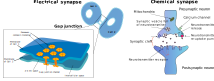
\includegraphics{img/intro/synapses.png}
    \caption{Representation of synapses types. Left. Example of electrical synapse structure. Right. Example of chemical synapse structure.}
    \label{fig:synapse-types}
\end{figure}

% As said there are many different ways to study neural dynamics, but a common descriptor for neural activity are action potentials. Action potentials are the 
Neural activity is often described by the potential alteration in the membrane caused by the flow of ionic channels and the conduction of nerve impulses by the axon. This variation of potential is called action potentials or spikes. We can see this as the minimal piece of information in the process of information reception, modification and transmission carried out by the neurons. A more concrete definition of spike could be "an abrupt and transient change of membrane voltage that propagates to other neurons via a long protrusion called an axon" \parencite{izhikevich_dynamical_2007}. Thus when no activity is transferred through the axon, the potential is called resting potential, main alterations to this potential are depolarization, when the potential is less negative than the resting potential, and hyperpolarization, when the potential is more negative than the resting potential. In figure \ref{fig:action potential} these potential phases are depicted. 

\begin{figure}[htb!]
    \centering
    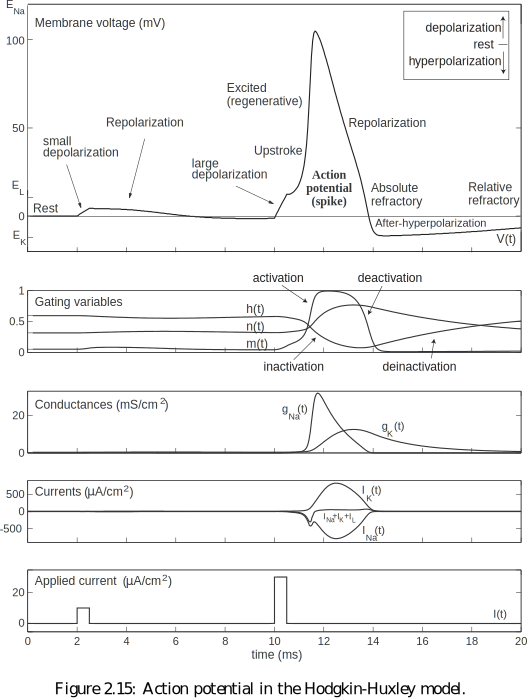
\includegraphics[width=\linewidth]{img/intro/dns_spike_phases.pdf}
    \caption{Representation of phases and terminology of an action potential. Adaptation of \textit{Figure 2.15: Action potential in the Hodgkin-Huxley model.} from book "Dynamical systems in neuroscience" \parencite{izhikevich_dynamical_2007}. }
    \label{fig:action potential}
\end{figure}
The membrane can be composed by different ionic channels, and its dynamics are conditioned by that combination and the possible synaptic connections. This changes in dynamics can be manifested in different ways, but the most notorious ones are the shape of the action potential and the type of activity that they show. %p61 The Neuron 
For example, in Figure \ref{fig:spike-types} there is an example of two distinct action potentials with visible differences in their shape. In Figure \ref{fig:spike_activity-types} there is an example of distinct neural activities from intracellular recordings. 
\begin{figure}[htb!]
    \centering
    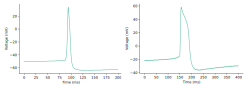
\includegraphics[width=\linewidth]{img/intro/spike-types.pdf}
    \caption{Examples of different spike shapes. Representation of two recordings from two different cells in \textit{Lymnaea stagnalis}. Left: symmetrical spike; right: shoulder shaped spike.}
    \label{fig:spike-types}
\end{figure}
\begin{figure}[htb!]
    \centering
    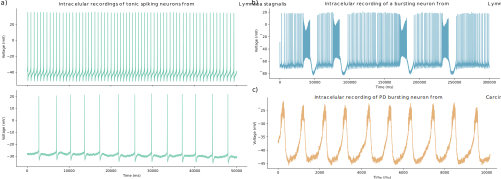
\includegraphics[width=\linewidth]{img/intro/spike_activity-types.pdf}
    \caption{Representation of different spiking activities. Left: two simultaneous intracellular recordings in \textit{Lymnaea stagnalis} showing tonic firing at two different frequencies. Right: Two examples of bursting activity, up from \textit{Lymnaea stagnalis} and bottom from \textit{Carcinus maenas}}
    \label{fig:spike_activity-types}
\end{figure}
If spikes are considered minimal pieces of information when coding the neural activity, the combination of these minimal information leads to new forms of information, also known as bursts. Although there is not a fixed description of a burst, and depending on the animal and system a burst might look different \parencite{russell_bursting_1978,palmu_detection_2010,lundqvist_gamma_2016}, there are some common features in bursts: combination of spikes (more than two), higher frequency, sustained depolarization, a hyperpolarization followed by a resting inter-burst period (IBI). Traditionally, neural code has been studied as information by the binarization of the activity i.e. an spike does or does not occur. Burst can also be part of this codification, either as a whole piece of information or as a complex box of data itself. "bursts are a family of firing patterns that trigger physiological mechanisms not engaged by the same number of spikes in relative isolation" \parencite{friedenberger_silences_2023}. Bursts can be originated either by internal activation, mostly by calcium channels or by the synaptic dynamics involving the corresponding cell (inhibition/excitation) (for an extended review see \parencite{friedenberger_silences_2023}). This is the case in Central Pattern Generators (CPGs) \parencite{Katz,steuer_central_2018} that will be discussed in detail bellow and in Chapter \ref{c-invariants-model}.

\section{The importance of sequential neural dynamics}
%the complex landscape of unanswered questions in the field of neuroscience, from a bottom-up approach. 
In the complex landscape of neuroscience, its study and conceptualization can be framed in three parts: hierarchy, if the study is bottom-up or top-down approach; ; and sequentiallity Among all the studies here present there is a common key: sequentially in neural dynamics. We can see most dynamics in the whole brain and behavior as a sequence of interactions, from molecules to motor movement. In this section we well see a review of the sequential nature of neurons and their information processing.

The structural differentiation in the 

% There are many important cognitive processes that rely in sequential processes such as perception, memory, decision making, attention and emotion. %Binding \parencite{Michel and coegin 2018, Ravinovich 2020, He 2018}.
% Sequentiallity involves complex pieces of dynamical activity, that when incapsulated as units, can be seen as a chain of events with sequential behaviour \parencite{Ravinovich,2023}.


% Sequential activvation for unsuppervised learning/activity.

Principles of Brain Dynamics: Global State Interaction Book
https://www.frontiersin.org/articles/10.3389/fnsys.2014.00219/full
https://www.ncbi.nlm.nih.gov/pmc/articles/PMC8367843/


%Kiebel 2009
%"Dynamic sequences are generated on various time-scales"
%"Brain is a recognition system that uses an internal model of its environment"

%Kiebel 2008
%"Many aspects of brain function can be understood in terms of a hierarchy of temporal scales at which representations of the environment evolve"


Temporal processing can be defined as the decoding of a generated temporal code. A common example of temporal processing is usually the speech processing, where temporal structures play a key role \parencite{bibid}. Sequential patterns are present in the phrases structure, as a sequences of syllables and silences. In this line, an extended case of study is the birdsong, which has this similarity to human's speech, as they process sequences of syllables \parencite{fishbein_sound_2019}. Beyond speech, sequential processing is also present in the motor movement and coordination, from muscle activation to repetitive movements such as rhythmic tapping.

The sequential activity in brain goes from the scale of microsecond to days, as it is the example of circadian rhythms (see \cite{mauk_neural_2004}). We can also see this in the generation of coordinated motor activity as it is the case of the feeding of a snail. At the scale of microseconds, there is a flow of ions that generate a sequence of ionic channel activation, that in the scale of milliseconds, produce that produce action potentials that activate the corresponding muscles at the scale of seconds  and generate the necessary sequential movement to eat: open the mouth, rasp food and swallow. In figure \ref{fig:time scale feeding} there is an illustration of these scales.

\begin{figure}[hbt!]
	\includegraphics[width=\textwidth]{img/intro/time scale/time-scale-feeding.pdf}
\end{figure}


However, it is not clear how exactly the brain processes time. In contrast to the theory of a central clock that manages time for every behavioral task, it is extended the theory of a distributed time processing \parencite{buonomano_temporal_1995,ivry_representation_1996}. For that to be processed, but maintaining effective responses, especially in movement, there is a need of circuits that manage the sequential movement.\todo{bibliografía} This is the case of Central Pattern Generators (CPGs), these are closed circuits of neurons that activate sequentially, in mutual inhibition and that generate coordinated motor activity in many systems, from insects to humans \parencite{bibid}. There are a few key aspects that makes this circuit an interesting case of study. First, the neurons in the closed-topology are able to maintain a rhythmic activity in an autonomous manner by mutual inhibition. Second, the activity is flexible enough to adapt to changes in the context, e.g., variations in the terrain while walking. Finally, it is present in many systems and in some of them there is a direct transcription between the neurons in the circuit and the motor movement they produce, e.g., the PD, LP and PY neurons in the stomatogastric CPG in the crab \textit{C. maenas} correspond to the pilo


\section{Computational Neuroscience}
Computational Neuroscience is a subfield of neuroscience that enhances the theoretical and computational techniques to address the study of nervous system functioning at multiple levels, from molecular level to complex networks or behavior. It is then by definition, a multi-disciplinary field. The basis of Computational Neuroscience lay on the understanding of brain dynamics from its electrical signals and the information they carry \parencite{schwiening_brief_2012,catterall_hodgkin-huxley_2012,dimitrov_information_2011,shannon_mathematical_1948}. Computational Neuroscience has extended its scope, leading to new paths o	f research including complex networks, graph theory, single cell analysis and machine learning techniques \parencite{cns2023}. Actually, in fields such as Artificial Intelligence there is a symbiotic relationship between fields, where both inspire and help each other grow \parencite{amunts_human_2019,wozniak_deep_2020,goncalves_training_2020}.

An important part of Computational Neuroscience is the description of living dynamics with theoretical models and the reproduction of their activity by the model simulation. The simulation of neural activity is a powerful tool to explore the neuronal dynamics, biophysical sources and possible mechanisms underlying the neural signaling, behavior, etc. Its strength relies on the reproducibility, extensive range of tunable parameters and the ability to modify (include/exclude) elements in the system or circuit. Like science is not about truth, but about knowledge, models do not aim to substitute living systems, but to lead us closer to the insight of neural dynamics. %#ToDo revisar

Models can be classified by their level of specification, i.e. what level of abstraction is decided in neural dynamics, the structure being modeled and the size of network and their ability to reproduce chaotic activity. In Figure \ref{fig:models-classification} there is a colored box illustrating this classification, with examples of models of large networks as \cite{potjans2014,bezaire2016}, of single cell but still detailed as in \cite{smith2013} and more abstract descriptions as in \cite{izhikevich}.


%Adapt models table from
%https://www.sciencedirect.com/science/article/pii/S0896627319304441 Figure 2A:
\begin{figure}[bth!]
	\centering
	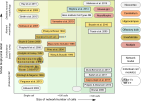
\includegraphics[width=\textwidth]{img/intro/models classification.pdf}
	\caption{Neural and network models classified by biophysical detail, structure modeled. Figure adapted from Figure 2 \cite{gleeson_open_2019}}
	\label{fig:models-classification}
\end{figure}
Although it was included in this classification, the capability of models to reproduce chaotic activity is often undervalued. Most studies use deterministic non-chaotic models, which are sufficient when exploring input/output responses, studying the role of different biophysical elements or supporting experimental results. However, living systems are chaotic and highly variable, and still able to produce sequential, constant and reproducible patterned activity. While this is a key aspect in neural dynamics, models usually exclude the variability from their description and include, when necessary Gaussian noise as external input to induce stochasticity. However, this is limited when exploring the role of variability in the sequences or in the information processing, inferring hypothesis from the model analysis.
\todo{mejorar justificación y añadir referencias de gaussian}
%#ToDo mejorar justificación y añadir referencias de gaussian.

\subsubsection{Conductance-based models}

In this thesis, all experimental recordings have been supported with simulations on conductance-based models. They can be defined as mathematical descriptions of the ionic channels dynamics, based on their electrical signal. The first description is usually assigned to \cite{hodgkin_quantitative_1952} model, that defined dynamical equations based on the electrical circuit of neurons in \textit{Aplysia}, see \ref{fig:electrical circuit}.

\begin{figure}[htb!]
	\centering
	\includegraphics[width=0.7\textwidth]{./img/intro/dns_neuron_circuit.pdf}
	\caption{Electrical circuit representing membrane. Figure 2.3 from book "Dynamical systems in neuroscience" from \cite{izhikevich_dynamical_2007}.}
	\label{fig:electrical circuit}
\end{figure}

In this models, the simulation of neural electrical activity is based on the combination of different ionic channels, whose dynamics are also well defined with a description of activation gates which are also dynamically defined. The equations correspond to the following structure:

Dynamical Voltage time dependent:

\begin{equation}
 C_m \frac{dV}{dt} = I - \sum I_{x},
\end{equation}

where $I_{x}$ is the current description for each channel involved in the action potential generation, e.g. $I_K$, $I_{Na}$, $I_{Ca}$.

Each channel is also described as a differential equation, voltage-dependent composed by activation-gates dynamics:
\begin{equation}
I_x =  g_x \sum act_{vars}^n (V - E_x), 
\end{equation}

where $g_x$ is the corresponding conductance of the channel, $E_x$ is the reversal potential for that channel.
Activation gates usually have an exponential tendency, and are defined by activation and inactivation dynamics, also dependent on voltage and time. They follow the structure in equation \ref{eq:alpha-beta}

\begin{equation}
	\label{eq:alpha-beta}
	\frac{act}{dt} = \frac{act{\inf,i}-act_i}{\tau_{act,i}}
\end{equation}

where $\tau_{act,i}$ are the relaxation time constants which are usually voltage-dependent and modeled using sigmoid or Gaussian functions, as in equations \ref{eq:alpha-beta}. 


 An example of the equations corresponding to figure \ref{fig:electrical circuit} are:
\begin{equation}
		C V = I - g_K n^4 (V - E_K) - g_{Na} m^3h(V-E_{Na}) - g_L (V-E_L)
\end{equation}

\begin{multicols}{2}
	\begin{equation}
		n = \alpha_n (V)(1-n)-\beta_n(V)n
	\end{equation}
	\begin{equation}
		m = \alpha_m (V)(1-m)-\beta_m(V)m
	\end{equation}
	\begin{equation}
		h = \alpha_h (V)(1-h)-\beta_h(V)h
	\end{equation}


	\begin{equation}
	\alpha_n(V)=0.01\frac{10-V}	{\exp(\frac{10-V}{10})-1}
	\end{equation}
	\begin{equation}
	\beta_n(V)=0.0125\exp(\frac{-V}{80})
	\end{equation}


\vspace{-15pt}
	\begin{equation}
		\alpha_m(V)=0.1\frac{25-V}{\exp(\frac{25-V}{10})-1}
	\end{equation}
	\begin{equation}
		\beta_m(V)=4\exp(\frac{-V}{18})
	\end{equation}

\vspace{-15pt}
	\begin{equation}
	\alpha_h(V)=0.07\exp\frac{-V}{20}
	\end{equation}
	\begin{equation}
		\beta_h(V)=\frac{1}{\exp(\frac{30-V}{10})+1}
	\end{equation}
\end{multicols}


As in living systems, the combination of different channels lead to different activities, e.g. shoulder and no-shoulder type neurons showed in Figure \ref{fig:spike-types}, can be reproduced in models (see Fig. \ref{fig:spike-types model}). 

\begin{figure}[htb!]
	\includegraphics[width=\textwidth]{img/intro/spike-types model.pdf}
	\caption{text}
	\label{fig:spike-types model}
\end{figure}



\section{Study in invertebrates}
\label{c-intro-invertebrates}
Even before computational techniques were an option, the study of Neural dynamics and behavior was carried using many different model animals. Apart from the hegemonic rodents models, there have been invaluable findings using invertebrates as animal models, such as genetics and developmental biology in \textit{C. elegans} \parencite{brenner_genetics_1974}, \textit{Zebra fish} \parencite{streisinger_production_1981} and \textit{Drosophila} \parencite{nusslein-volhard_mutations_1980}; neural dynamics in \textit{Aplysia} \parencite{HODGKIN1952,wachtel_direct_1967}, motor activity in \textit{Carcinus maenas} \parencite{eisen_mechanisms_1982} or \textit{Lymnaea stagnalis} \parencite{Benjamin1979b}, the main animal model in this thesis. Those are only examples of fields, these animal models have been used for a wide variety of fields including behavioral studies, ecotoxicology, evolution, human disease modelling... \parencite{romanova_animal_2018} 

Despite the differences between invertebrates, mammals and concretely human brain, there are many characteristics of animals' systems that can be extrapolated to humans. In fact, there are differences even in mammal species \parencite{preuss_taking_2000}, so by exploring more animal species there can be set a better ground truth for the aspects that shape the neuronal and behavioral dynamics. 

 % https://karger.com/bbe/article-abstract/55/6/287/46613/Taking-the-Measure-of-Diversity-Comparative?redirectedFrom=fulltext  
 %First, by examining a wider range of species than are currently employed, and by using modern techniques of phyletic analysis, neuroscientists can more rigorously identify those features of cortical organization that are, in fact, widely shared among mammals or among particular mammalian subgroups. Second, by taking account of variations, neuroscientists can abstract more reliable and general principles of structure-function relationships in the nervous system. Finally, freed from the doctrine of basic uniformity, neuroscientists can pursue the study of human cortical specializations, and so advance our understanding of what distinguishes humans as a biological species.

Among the advantages in using invertebrates there are the easy access to the nervous system, the ease of breeding and reproduction, the simplicity of their biological features, making a full description possible, i.e. the genomic description of \textit{C. elegans} or the nervous system in \textit{Lymnaea stagnalis}. Also some selected species were a main field of study in the last decades, so there is plenty of literature for each one even in different fields. Furthermore, despite the simplicity of these systems, their nervous system is still capable of generating robust sequential neural activity, preset behavior and even learning processes. 

Findings in invertebrates are sometimes overlooked, arguing that features in invertebrates cannot be extrapolated to humans. Thus, there are often used mammals by their biological similarity. However, models in invertebrates have proven their utility not only in basic science. We can find examples of this in human diseases, memory, motor activity and neuromodulation. Particularly, in the study of neural processes, the ease of accessibility and finite number of large neurons in the system, have made invertebrates an interesting case of study. In Figure \ref{fig:invertebrates timeline} there is a timeline containing crucial discoveries in Neuroscience, some of them Nobel Prize winners in the last century, as well as current relevant discoveries in the field. 
% https://docs.google.com/spreadsheets/d/16rOG5LSuFMQGHAakeYqcdG26NIZnY4NWtr6TZku_UKs/edit#gid=0

Apart from the possible advances in science, invertebrates models can also bridge the gap between resources and science, allowing low-income labs and countries to do science. This animal models are usually cheaper to obtain, maintain and there is usually a possibility of breeding own colonies. This makes their use extendable and breaks some economical barriers in science, where high-income countries usually centralize the science production with strong conventions \parencite{castillo_spineless_2017,stephan_how_2015}. 

\textit{What can computational neuroscience provide to experimental approaches}



\subsubsection{\textit{Lymnaea stagnalis}, the great pond snail}
Besides the potential of research in invertebrates in general, here we explore neural system in the great pond snail, \textit{Lymanea stagnalis}. This mollusk has been an important case of study since the late XX century, when it was used extensively to study neurobiological processes and nervous system functioning \parencite{Benjamin1979a}. %#TODO: repaso de Benjamin

\begin{wrapfigure}{l}{0.3\textwidth}
	\centering
	\includegraphics[width=0.7\linewidth]{img/intro/lymnaea.png} 
	\caption{\textit{Lymnaea Stagnalis}}
	\label{fig:snail}
\end{wrapfigure}  From that point on it has been key in other fields as host-parasite or genome editing. This last field is thanks to the short and well studied life-cycle in \textit{L. stagnalis} (see Figure \ref{fig:lymnaea_life_cycle}), as well as the easiness to lab-bread them, without losing its main characteristics through generations \parencite{noland_observations_1946}. 


\begin{figure}[htb!]
	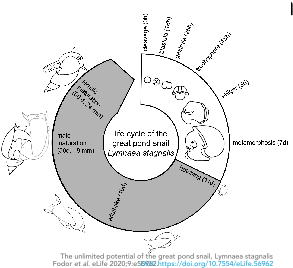
\includegraphics[width=\textwidth]{img/intro/lymnaea_life_cycle.pdf}
	\caption{text}
	\label{fig:lymnaea_life_cycle}
\end{figure}




\section{Neuromodulation and its need for clinical applications}
 \chapter{Introducción y Estado del Arte}
\label{c-intro spanish}

\section{Neurociencia, neuronas y su dinámica}
% \textit{¿Qué son las neuronas, su dinámica y cuáles son las tareas pendientes?}
La neurociencia es un campo amplio y desafiante. Afronta preguntas cruciales, tales como el estudio de los mecanismos neuronales subyacentes a la actividad cerebral, cómo pueden esos mecanismos resultar en procesos cognitivos o el comportamiento humano, cómo la información se percibe, procesa, transforma y crea, y finalmente se convierte en acciones a través de la actividad neuronal, cómo se originan las enfermedades neuronales y cómo podemos detectarlas y tratarlas. 
Estas preguntas y muchas más han sido problemas abiertos que han intrigado a la comunidad científica desde los primeros pasos en el campo. La neurociencia nació como una disciplina moderna a partir de la anatomía, la fisiología, la bioquímica y la biofísica. Por el amplio rango del campo, se suele abordar desde distintas perspectivas y comunmente se referencia por sus subcampos, por ejemplo, Neurobiología, Neurofarmacología, Neurociencia Clínica, Neurociencia del Desarrollo, Neurociencia de Sistemas, Neurociencia Cognitiva, Neurociencia Computacional, Neurotecnología, etc. Todos estos campos tienen como objetivo explicar o reparar la función cerebral, ya sea en su totalidad o parcialmente. En este proceso se utilizan diferentes técnicas y enfoques, algunos de los cuales dan lugar a campos completamente nuevos, como la Neuroimagen.

No podemos pensar o discutir sobre neurociencia sin destacar el trabajo de Santiago Ramón y Cajal, crucial en los primeros pasos para comprender el cerebro \parencite{ramonycajal_textura_1899,decarlos_historical_2007,decastro_editorial_2016,delgado-garcia_cajal_2015,decastro_cajal_2019}. La idea de la "doctrina de la neurona" fue un impulso en el estudio del cerebro, explicando y describiendo la estructura de células individuales llamadas \textit{neuronas} que son capaces de conectarse y, por lo tanto, comunicarse mediante \textit{sinapsis}. La Figura \ref{fig:cajal-neuron spanish} muestra uno de los dibujos de Cajal que ilustra la retina de la abeja y una primera aproximación al posible curso del flujo de información en este sistema.

\begin{figure}[htb!]
    \centering
    \includegraphics[width=0.3\textwidth]{img/intro/cajal-flow_small.jpg}
    % https://es.wikipedia.org/wiki/Doctrina_de_la_neurona#/media/Archivo:CajalCerebellum.jpg
    % https://microbioblog.es/la-fascinante-historia-de-la-reazione-nera
    \caption{Ilustración de Ramón y Cajal que muestra el posible curso de información en la retina de la abeja. \parencite{ramonycajal_sobre_1915} (Disponible bajo la licencia: \href{https://creativecommons.org/licenses/by-sa/4.0/}{CC BY 4.0})}
    \label{fig:cajal-neuron spanish}
\end{figure}
%Desde ese punto de partida ha habido hallazgos importantes en los tipos y estructuras de neuronas, como las células gliales \ref{}.

El cerebro es un sistema complejo que podemos estudiar desde diferentes prismas. En esta tesis, seguimos un enfoque \textit{bottom-up} (de abajo hacia arriba), en el que analizamos de forma experimental y teórica la actividad neuronal desde una descripción de la dinámica de canales iónicos y la de pequeños circuitos (con pocas sinapsis). Además, seguimos una perspectiva neurocomputacional basada en el procesamiento secuencial jerárquico de la información, que se definirá en detalle en la subsección \ref{sec:computational neuroscience spanish}. En las siguientes líneas abordaremos las bases de la activación neuronal desde esta perspectiva computacional necesaria para la comprensión de este documento. Nos centraremos en la dinámica de voltaje que las neuronas son capaces de producir y en su interrelación para dar lugar a su actividad secuencial colectiva.


\subsection{Dinámica neuronal}
Las neuronas son células morfológicamente compuestas por dendritas, donde se reciben las conexiones de otras neuronas a través de sinapsis; un soma o cuerpo celular (donde normalmente se integra la información) y un axón (donde la información se transmite como salida). Dado que las neuronas son las células que presentan la mayor diversidad en morfología, esta descripción no se aplica a todos los tipos neuronales, pero nos sirve para comenzar a destacar la importancia de las escalas espaciales en el sistema nervioso.

% Como se mencionó, hay muchas formas diferentes de estudiar la dinámica neuronal, pero un descriptor común de la actividad neuronal son los potenciales de acción. Los potenciales de acción son el
La actividad eléctrica neuronal a menudo se describe en términos de la evolución del voltaje de la membrana causada por el flujo de canales iónicos entre el interior y el exterior de la célula \parencite{kandel_principles_2012}. El cambio rápido característico en el voltaje de la membrana cuando una neurona emite una señal de salida se llama potencial de acción o \textit{spike}. Estos potenciales de acción suelen considerarse como la unidad mínima de información para la recepción, procesamiento y transmisión por parte de las neuronas. Una definición más concreta de \textit{spike} podría ser "un cambio abrupto y transitorio del voltaje de la membrana que se propaga a otras neuronas a través de una extensión larga llamada axón" (traducción con del texto original) \parencite{izhikevich_dynamical_2007}. Así, cuando no se reciben entradas, el potencial de la membrana de una neurona es negativo y se llama potencial de reposo. Cuando este potencial se altera por una entrada que hace que el voltaje aumente, se conoce como despolarización. Después de alcanzar un pico de voltaje, típicamente un valor positivo de alrededor de 40mV, el potencial comienza a disminuir nuevamente. Cuando el potencial es más negativo que el potencial de reposo, se conoce como hiperpolarización. La Figura \ref{fig:action potential spanish} ilustra las fases secuenciales de la generación del potencial de acción.

\begin{figure}[htb!]
	\centering
	\includegraphics[width=0.8\textwidth]{img/intro/action_potential.pdf}
	\caption{Representación de las fases secuenciales y terminología de un potencial de acción. (Adaptado de Chris73, Wikimedia Commons, \href{https://creativecommons.org/licenses/by-sa/3.0/}{CC BY-SA 3.0}). En cada una de estas fases de la generación del potencial de acción, se activan secuencialmente diferentes canales iónicos, por ejemplo, el canal de sodio está involucrado durante la fase de despolarización y su actividad disminuye a medida que el canal de potasio se activa principalmente en la fase de repolarización.}
	\label{fig:action potential spanish}
\end{figure}

La actividad neuronal se produce por el flujo de diferentes canales iónicos que provocan la generación de potenciales de acción \parencite{koch_biophysics_1999}. La membrana puede estar compuesta por diferentes canales iónicos, y su dinámica está condicionada por esa combinación y las posibles conexiones sinápticas a las que está sujeta la neurona. Estos cambios en la dinámica se ponen de manifiesto de diferentes maneras, pero las más representativas son la forma de onda y la evolución temporal de los potenciales de acción. %p61 The Neuron
Por ejemplo, en la Fig. \ref{fig:spike-types spanish} muestra dos potenciales de acción distintos con diferencias visibles en su forma de onda. En la Figura \ref{fig:spike-types spanish}a) se muestra un potencial que presenta una forma simétrica, donde las pendientes de despolarización y repolarización son similares, mientras que en la forma de onda de Fig. \ref{fig:spike-types spanish}b), hay un "hombro" característico en la repolarización y su escala temporal es casi el doble en comparación con el ejemplo mostrado en la Fig. \ref{fig:spike-types spanish}a).

\begin{figure}[htb!]
	\centering
	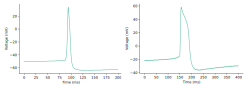
\includegraphics[width=\linewidth]{img/intro/spike-types.pdf}
	\caption{Ejemplos de diferentes formas de \textit{spikes}. Representación de dos registros de dos células diferentes en el ganglio parietal derecho de \textit{Lymnaea stagnalis}. a) \textit{Spike} con forma de onda simétrica; b) \textit{Spike} con forma de onda con "hombro".}
	\label{fig:spike-types spanish}
\end{figure}

Si consideramos los potenciales de acción como piezas mínimas de información al codificar la actividad neuronal, la combinación de estas piezas mínimas de información lleva a nuevas formas de información, también conocidas como ráfagas. Aunque no hay una descripción fija de una ráfaga, y dependiendo del animal y el sistema una ráfaga puede verse diferente \parencite{russell_bursting_1978,palmu_detection_2010,lundqvist_gamma_2016}, hay algunas características comunes en ellas: normalmente consisten en un grupo de \textit{spikes} (más de dos) sobre una despolarización sostenida, y estos grupos están separados por un período de quiescencia de hiperpolarización llamado intervalo entre ráfagas (IBI). La Figura \ref{fig:spike_activity-types spanish} muestra varios ejemplos de distintas actividades neuronales observadas en grabaciones intracelulares. Dependiendo de la neurona específica y el circuito, las neuronas pueden presentar disparo tónico (primera columna), a diferentes velocidades, o actividad en ráfagas (segunda columna).

\begin{figure}[htb!]
	\centering
	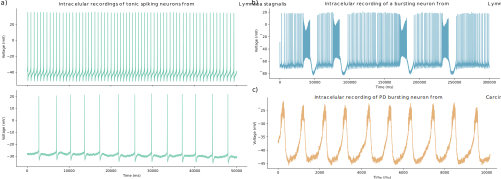
\includegraphics[width=\linewidth]{img/intro/spike_activity-types.png}
	\caption{Representación de dos ejemplos de diferentes actividades neuronales de disparo. Izquierda: dos grabaciones intracelulares simultáneas en \textit{Lymnaea stagnalis} mostrando disparo tónico a dos frecuencias diferentes. Derecha: Dos ejemplos de actividad en ráfagas, de registros intracelulares en \textit{Lymnaea stagnalis} (panel superior) y en \textit{Carcinus maenas} (panel inferior).}
	\label{fig:spike_activity-types spanish}
\end{figure}

Tradicionalmente, los códigos neuronales se han estudiado centrándose en la activación de \textit{spikes} individuales, por ejemplo, mediante la binarización de la actividad (la neurona genera un \textit{spike} o no). Las ráfagas también pueden ser informativas en términos de la actividad neuronal, ya sea como una pieza completa de información o como una caja de datos compleja en sí misma: "las ráfagas son una familia de patrones de disparo que desencadenan mecanismos fisiológicos que no se activan con el mismo número de \textit{spikes} en relativo aislamiento" \parencite{friedenberger_silences_2023}. Las ráfagas pueden originarse por activación interna, principalmente por canales de calcio y/o por la dinámica sináptica que involucra a la célula correspondiente (inhibición/excitación), para una revisión extendida ver \parencite{friedenberger_silences_2023}. La actividad en ráfagas es muy común en circuitos Generadores Centrales de Patrones (CPGs) \parencite{katz_evolution_2016,steuer_central_2018}, que se discutirán en detalle a continuación y en el Capítulo \ref{c-invariants}.

\subsection{Dinámicas de redes}

Aunque el análisis de la actividad de una sola neurona es importante para caracterizar su dinámica, cuando se habla de procesamiento de información y comportamiento, también es crucial estudiar la dinámica general del circuito. Un circuito de neuronas se define por células nerviosas interconectadas por sinapsis. Existen dos tipos principales de sinapsis en el sistema nervioso: conexiones eléctricas y químicas, como se muestra en la Fig. \ref{fig:synapse-types spanish}. La principal diferencia entre ellas radica en cómo se lleva a cabo la comunicación. Las sinapsis químicas ocurren mediante la mediación de \textit{neurotransmisores}, donde una neurona presináptica libera estas moléculas que se unen a los neuroreceptores para producir una alteración en la neurona postsináptica. Por lo tanto, esta conexión es asimétrica y unidireccional, mientras que en las sinapsis eléctricas encontramos una conexión simétrica y bidireccional. En estas sinapsis, las neuronas están casi unidas por una estructura llamada \textit{unión gap} (\textit{gap junction} en inglés), que conecta ambas neuronas en una estructura tisular que limita la fuga al espacio extracelular. Esta comunicación permite que la carga eléctrica fluya de una neurona a otra y es más rápida que las sinapsis químicas, con una comunicación sin retraso en comparación. La actividad de las neuronas acopladas eléctricamente suele ser sincrónica \parencite{levitan_neuron_2002}.

\begin{figure}[hbt!]
	\centering
	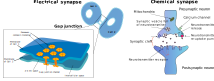
\includegraphics[width=\linewidth]{img/intro/synapses.pdf}
	\caption{Representación de tipos de sinapsis. Izquierda: Ilustración de una sinapsis eléctrica entre dos células y diagrama de unión estrecha (Adaptado de \href{https://commons.wikimedia.org/wiki/File:Gap_cell_junction-en.svg}{Wikimedia Commons}). Derecha: Ilustración de la estructura de una sinapsis química (Adaptado de \href{https://commons.wikimedia.org/wiki/File:Synapse_diag1.svg}{Wikimedia Commons})}
	\label{fig:synapse-types spanish}
\end{figure}

Las neuronas pueden estar conectadas varios tipos de sinapsis químicas y eléctricas, y generalmente también están conectadas a otros circuitos bajo el efecto de neuronas moduladoras. La Figura \ref{fig:neural circuits spanish} ilustra dos ejemplos de circuitos a nivel celular y macroscópico. En cualquier sistema nervioso, se forman conglomerados complejos de redes de redes, que pueden funcionar a diferentes escalas temporales y pueden participar en multiples funcionalidades. Esta interconexión de redes y, a un nivel más bajo, de células, conduce a activaciones secuenciales y transferencias de acciones en secuencias de secuencias \parencite{rabinovich_sequential_2020}.

\begin{figure}[hbt!]
	\centering
	\includegraphics[width=0.64\textwidth]{img/intro/cpg diagram.png}
	\includegraphics[width=0.35\textwidth]{img/intro/The_Human_Connectome.png}
	\caption{Izquierda: Esquema de la conectividad del CPG pilórico y gástrico del crustáceo, probablemente uno de los circuitos mejor conocidos en neurociencia \parencite{huerta_topology_2001}. Derecha: Conectoma en el cerebro humano renderizado a partir de 20 sujetos (Por Andreashorn - Trabajo propio,\href{https://commons.wikimedia.org/w/index.php?curid=41581320}{CC BY-SA 4.0})}
	\label{fig:neural circuits spanish}
\end{figure}

\section{La naturaleza secuencial de la dinámica neuronal}

Las dinámicas cerebrales pueden describirse como secuencias de interacciones, desde moléculas, hasta neuronas, control motor y comportamiento, implicando una jerarquía coordinada de escalas temporales y espaciales \parencite{kiebel_hierarchy_2008,yuste_cortex_2005,rabinovich_discrete_2018,rabinovich_neurons_2023}, desde activaciones de canales iónicos hasta codificación sensorial, procesamiento y toma de decisiones. Su estudio revela aspectos fundamentales de la función cerebral y la cognición, por ejemplo, la transmisión de impulsos, la función ejecutiva, el procesamiento espacial, memoria, etc.

Un ejemplo común de procesamiento secuencial es el habla, donde los patrones secuenciales están presentes en la estructura de las frases, como secuencias de secuencias de sílabas, palabras y silencios \parencite{kiebel_recognizing_2009}. En esta línea, un caso de estudio extendido es el canto de los pájaros, que tiene similitud con el habla humana, ya que involucran secuencias de sonidos coordinados \parencite{prather_brains_2017,fishbein_sound_2019}. Aparte de en el habla, el procesamiento secuencial también está presente en el control motor, desde la activación muscular hasta acciones coordinadas repetitivas como el golpeteo rítmico o la interpretación musical \parencite{ding_temporal_2017}. Además, hay muchos procesos cognitivos importantes que dependen de mecanismos secuenciales como la percepción, la memoria, la toma de decisiones, la atención y la emoción \parencite{varona_hierarchical_2016, he_robust_2018, rabinovich_sequential_2020}.

Sin embargo, no está claro cómo procesa exactamente el cerebro el tiempo. En contraste con la teoría de un reloj central que gestiona el tiempo para cada tarea conductual, la teoría de un procesamiento temporal distribuido \parencite{buonomano_temporal_1995,ivry_representation_1996} es bien aceptada. En este marco, especialmente en la coordinación del movimiento, existen circuitos que gestionan la actividad rítmica secuencial. Este es el caso de los Generadores Centrales de Patrones (CPGs), circuitos de neuronas con topología cerrada que activan secuencialmente neuronas y generan actividad motora coordinada \parencite{selverston_reliable_2000}. Están presentes en muchos sistemas, desde insectos hasta humanos \parencite{pearson_central_1972,marder_central_2001,mackay-lyons_central_2002,minassian_human_2017}. Hay varios aspectos clave que hacen de estos circuitos un caso de estudio interesante. Primero, sus neuronas están organizadas en topologías cerradas recibiendo retroalimentación de células compañeras \parencite{huerta_topology_2001}. Estos circuitos pueden mantener una actividad rítmica de manera autónoma, típicamente mediante interacciones inhibitorias mutuas \parencite{katz_evolution_2016}. Segundo, su actividad es lo suficientemente flexible como para adaptarse a cambios en el contexto, por ejemplo, variaciones en el terreno al caminar. Finalmente, están presentes en muchos sistemas y en algunos de ellos hay una relación directa entre la actividad de las neuronas en el circuito y el movimiento motor que producen. Por ejemplo, en el CPG pilórico en el cangrejo \textit{C. maenas}, encargado del movimiento del píloro, las neuronas PD (dilatador pilórico), LP (pilórico lateral) y PY (PYlórico) corresponden a la dilatación del píloro, el cierre del píloro y la contracción del constrictor rostral para mover los alimentos en el sistema digestivo \parencite{moulins_introduction_1987,selverston_oscillations_2006}.

\begin{figure}[hbt!]
	\centering
	\includegraphics[width=0.7\textwidth]{img/intro/time scale/time-scale-feeding.pdf}
	\caption{Ilustración del proceso de alimentación secuencial en diferentes escalas de tiempo en {\sl Lymnaea stagnalis}.}
	\label{fig:time-scale feeding spanish}
\end{figure}

La actividad secuencial en el cerebro va desde la escala de sub-milisegundos hasta días (la escala temporal de los ritmos circadianos \parencite{mauk_neural_2004}). La Figura \ref{fig:time-scale feeding spanish} muestra un ejemplo ilustrativo de la naturaleza secuencial de la actividad neuronal en diferentes escalas en la generación de actividad motora coordinada en la alimentación de un caracol. A la escala de sub-milisegundos, hay un flujo de iones que genera una secuencia de activación de canales iónicos, que en la escala de milisegundos produce potenciales de acción. La combinación de ellos en forma de ráfagas rítmicas, activa los músculos correspondientes en la escala de segundos y genera el movimiento secuencial necesario para alimentarse: abrir la boca, raspar el alimento y tragar, que se repite a lo largo del día.

El estudio de la dinámica de los potenciales de acción y la interacción entre los canales iónicos y las sinapsis es crucial, ya que es una parte clave en cualquier proceso cerebral, y no puede separarse del estudio de la actividad en su conjunto. La alteración de la dinámica de estos canales a diferentes niveles, puede afectar las entradas/salidas sinápticas, cómo se comunican las neuronas y el proceso resultante. Los canales iónicos son el punto de partida de las señales eléctricas subyacentes a la actividad de la red neuronal, y su mal funcionamiento puede contribuir a trastornos neuronales \parencite{kecskes_editorial_2023}. Por lo tanto, comprender la actividad cerebral no solo a gran escala sino también desde la etapa de generación de dinámicas de voltaje puede ser clave para una comprensión realmente completa de los sistemas neuronales. Su estudio también puede ayudar a distinguir entre la modulación a corto y largo plazo, un aspecto clave en la plasticidad neuronal y la aplicación de técnicas neuromoduladoras \parencite{chambers_lightactivated_2008,burke_modulation_2019}.

Es importante explorar los mecanismos que permiten mantener una actividad secuencial robusta a pesar de los cambios en el contexto informacional mediante la entrada de diferentes estímulos y la variabilidad subyacente en la dinámica neuronal. Los potenciales de acción y las ráfagas pueden clasificarse según su forma de onda y la actividad de disparo agrupada. Sin embargo, en esos subgrupos hay una alta intra-variabilidad, donde, por ejemplo, la actividad de ráfagas puede diferir en forma y duración, es decir, en el número de potenciales en una ráfaga. La Figura \ref{fig:burst variability spanish} muestra un ejemplo de la variabilidad en la forma de onda y la duración de la ráfaga para una secuencia de varias ráfagas.

\begin{figure}[htb!]
	\centering
	\includegraphics[width=0.6\textwidth]{img/intro/burst_variability.png}
	\caption{Superposición de ráfagas en diferentes instantes de tiempo alineadas por el primer \textit{spike} en la ráfaga para grabaciones intracelulares de una neurona LP en el CPG pilórico.}
	\label{fig:burst variability spanish}
\end{figure}

El estudio de esta variabilidad revela factores clave en la secuencialidad y cómo se mantiene a pesar de diferentes modulaciones intrínsecas o externas. Este es el caso, por ejemplo, de los invariantes dinámicos secuenciales, es decir, relaciones robustas entre intervalos de tiempo que conforman una secuencia neuronal, al analizar la actividad ciclo a ciclo \parencite{reyes_artificial_2008,elices_robust_2019,garrido-pena_characterization_2021,berbel_emergence_2024}. Estos invariantes dinámicos secuenciales pueden tener un papel crucial en la coordinación de la actividad secuencial de forma autónoma, en el que se establece un equilibrio entre robustez y flexibilidad de sus intervalos temporales, requeridas para una función efectiva en muchos procesos cerebrales \parencite{tatsuno_analysis_2015,ullen_neural_2003,zimnik_independent_2021,zhou_neural_2020,dragoi_cell_2020}. Discutiremos en detalle este fenómeno en el CPG alimentario de \textit{Lymnaea stagnalis} en el capítulo \ref{c-invariants}.


\section{Estudio de la dinámica neuronal mediante modelos computacionales.}
\label{sec:neurociencia_computacional}
La Neurociencia Computacional es un subcampo de la neurociencia que utiliza técnicas teóricas y computacionales para abordar el estudio del sistema nervioso en múltiples niveles, desde el nivel molecular hasta redes complejas que dan forma al comportamiento. Es, por lo tanto, un campo multidisciplinario. La base de la Neurociencia Computacional radica en la comprensión de la dinámica cerebral a partir de sus señales eléctricas y la información que transportan \parencite{schwiening_brief_2012,catterall_hodgkinhuxley_2012,dimitrov_information_2011,shannon_mathematical_1948}. Desde sus comienzos, la Neurociencia Computacional ha ampliado su alcance, llegando a nuevos caminos de investigación que incluyen redes complejas, teoría de grafos, análisis de células individuales y técnicas de aprendizaje automático \parencite{_30th_2021}. En campos como la Inteligencia Artificial incluso existe una relación simbiótica entre ambos, en la que se inspiran y se ayudan mutuamente a crecer \parencite{amunts_human_2019,wozniak_deep_2020,goncalves_training_2020}.

Una parte importante de la Neurociencia Computacional es la descripción de sistemas neuronales con modelos teóricos y la reproducción de fenómenos clave mediante la simulación del modelo. La simulación de la actividad neuronal es una herramienta de gran potencial para explorar la dinámica neuronal, sus fuentes biofísicas, los posibles mecanismos subyacentes en la señal neuronal y el complejo procesamiento de la información observada. Su potencial radica en la completa accesibilidad a las variables del modelo, el rango típicamente extenso de parámetros ajustables en el modelo que se pueden explorar y la capacidad para evaluar el papel de elementos distintos en el sistema o circuito incluyéndolos o excluyéndolos de las simulaciones. Aunque los modelos no pueden sustituir completamente la investigación en sistemas vivos, sí nos acercan a la comprensión de la dinámica neuronal compleja, siendo una metodología conveniente, eficaz y de bajo coste para los avances científicos. Además, los modelos son un complemento esencial para la neurociencia experimental, alcanzando descripciones detalladas donde los enfoques experimentales como la electrofisiología tienen limitaciones debido a la observabilidad parcial subyacente al método.

Los modelos pueden clasificarse según su nivel de descripción, es decir, qué nivel de simplificación/abstracción se utiliza, el detalle de la estructura/fenómeno que se modela y el tamaño de la red, o su capacidad para reproducir la actividad neuronal observada, por ejemplo, dinámicas caóticas. La Figura \ref{fig:models-classification spanish} ilustra este tipo de clasificación, con ejemplos de modelos de grandes redes como \textcite{potjans_celltype_2014,bezaire_interneuronal_2016}, de células individuales pero aún detallados como en \textcite{smith_dendritic_2013}, y descripciones más abstractas como la propuesta en \textcite{izhikevich_simple_2003}. En cuanto al nivel de descripción, en los diferentes modelos biofísicos siempre hay una elección entre la descripción detallada de las no linealidades, canales y propiedades de excitación, y la eficiencia en la computación. En esta línea, los investigadores pueden elegir entre modelos basados en conductancia \parencite{hodgkin_quantitative_1952}, ricos en la descripción de no linealidades, o modelos dinámicos simplificados \parencite{hindmarsh_model_1984,fitzhugh_impulses_1961}, que típicamente representan no linealidades con simplificaciones polinomiales (ver \parencite{torres_modeling_2012} para una revisión de diferentes niveles de modelado neuronal).

\begin{figure}[bth!]
	\centering
	\includegraphics[width=\textwidth]{img/intro/models classification_v2.pdf}
	\caption{Modelos neuronales y de red clasificados por su nivel de detalle biofísico (los menos específicos están situados en la parte inferior del eje $y$), por estructura modelada (color de las cajas) y por el tamaño de la red (eje $x$). Figura adaptada de la Fig. 2 \parencite{gleeson_open_2019} bajo licencia \href{http://creativecommons.org/licenses/by/4.0/}{Creative Commons CC-BY}. Los modelos están clasificados por el detalle biofísico, siendo los modelos en la parte inferior los menos específicos; por el tamaño de la red modelada, de izquierda a derecha, una célula a cientos de células; y por la estructura cerebral que modelan, representada en cajas de colores. La forma de la caja también clasifica en modelo de red o célula individual. La espiral representa actividad caótica y ha sido incluida modificando la figura original. Una espiral en la caja indica la capacidad del modelo para producir actividad caótica sin alteraciones externas, es decir, reproducir variabilidad intrínseca espontánea. Aunque la figura no contiene todos los enfoques de modelos, ilustra hitos clave en el modelado neuronal.}
	\label{fig:models-classification spanish}
\end{figure}

\subsection{Modelos basados en conductancia}

En esta tesis, todos los registros experimentales se han complementado con simulaciones mediante modelos basados en conductancia. Estos se definen como descripciones matemáticas de la dinámica de los canales iónicos, basadas en su conductancia dependiente del voltaje. El estudio pionero de \textcite{hodgkin_quantitative_1952} definió ecuaciones dinámicas basadas en el circuito eléctrico equivalente de las propiedades eléctricas de las neuronas en el axón gigante del calamar, ver Fig. \ref{fig:electrical circuit spanish}. Este circuito también se puede utilizar para describir la configuración de registro intracelular, donde la pipeta se incluye como una corriente adicional compensada por el electrodo en la solución (ver Fig. \ref{fig:clamp circuit spanish}).

\begin{figure}[htb!]
\centering
\includegraphics[width=0.7\textwidth]{./img/intro/electrical_circuit.pdf}
\caption{Circuito eléctrico que describe el potencial de membrana en un modelo de neurona basado en conductancia.}
\label{fig:electrical circuit spanish}
\end{figure}

\begin{figure}[htb!]
\centering
\includegraphics[width=0.7\textwidth]{./img/intro/intracellular_recording_circuit.pdf}
\caption{Circuito eléctrico que representa el esquema para registros intracelulares.}
\label{fig:clamp circuit spanish}
\end{figure}

En estos modelos, la simulación de la actividad eléctrica neuronal se basa en la descripción matemática de diferentes canales iónicos en el circuito, cuya dinámica también está bien definida por compuertas de activación. Primero, hay una descripción matemática de la dependencia del voltaje en el tiempo, como se describe en la ecuación \ref{eq:voltage ions spanish}:

\begin{equation}
C_m \frac{dV}{dt} = - I - \sum I_{x},
\label{eq:voltage ions spanish}:
\end{equation}

donde \( V \) es el potencial de membrana, \( I \) es una corriente externa, por ejemplo, un estímulo externo o una corriente sináptica, \( I_{x} \) es la descripción de la corriente para cada canal involucrado en la generación del potencial de acción, por ejemplo, sodio, potasio, calcio (\( I_K \), \( I_{Na} \), \( I_{Ca} \)).

En segundo lugar, cada canal también se describe dependiente del voltaje compuesto por dinámicas de compuertas de activación:

\begin{equation}
I_x =  g_x m^n h^n (V - E_x),
\end{equation}

donde \( g_x \) es la conductancia máxima del canal, \( E_x \) es el potencial de reversión para ese canal y \( m \) y \( h \) representan las variables de activación e inactivación de la conductancia, respectivamente.
Estas variables suelen tener una descripción no lineal (tendencia exponencial) dependiente del voltaje y el tiempo. Siguen generalmente la estructura en la ecuación \ref{eq:alpha-beta spanish}:

\begin{equation}
\frac{dm}{dt} = \frac{m_{\infty} - m}{\tau_m}
\label{eq:alpha-beta spanish}
\end{equation}

donde $\tau_{m,i}$ son constantes de tiempo de relajación que suelen depender del voltaje y se modelan utilizando funciones sigmoides o gaussianas. Aunque aquí utilizamos $m$, esta fórmula también se aplica a las variables de inactivación.

Siguiendo el formalismo de Hodgkin y Huxley, las ecuaciones que describen la dinámica del voltaje y la dinámica de la conductancia de los canales activos (Na y K) en el circuito mostrado en la Fig. \ref{fig:electrical circuit spanish} se describen en la tabla \ref{table:hh-equations spanish}.

\begin{table}[h!]
	\begin{tabular}{lccc}
		Ecuación de voltaje                                                                 & \multicolumn{3}{c}{$C \frac{dV}{dt} = I - g_K n^4 (V - E_K) - g_{Na} m^3h(V-E_{Na}) - g_L (V-E_L)$}                                                                                                                                  \\ \hline
		& \multicolumn{2}{c}{Variables de activación}                                                                                                                              & Variable de inactivación                                        \\ \hline
		\multicolumn{1}{c|}{\begin{tabular}[c]{@{}c@{}}variables \\ de compuerta\end{tabular}} & \multicolumn{1}{c|}{$\frac{dm(t)}{dt}=\frac{m_{\infty}(V(t))-m(t)}{\tau_m(V(t))}$} & \multicolumn{1}{c|}{$\frac{dn(t)}{dt}=\frac{n_{\infty}(V(t))-n(t)}{\tau_n(V(t))}$} & $\frac{dh(t)}{dt}=\frac{h_{\infty}(V(t))-h(t)}{\tau_h(V(t))}$ \\ \hline
	\end{tabular}
	\caption{Ecuaciones del formalismo de Hodgkin y Huxley para la ecuación de voltaje y las variables de compuerta}
 \label{table:hh-equations spanish}
\end{table}

Esta combinación de canales genera la forma de la espiga mostrada en la Fig. \ref{fig:spike-types model spanish}a pero, como en las neuronas vivas, la combinación de diferentes canales conduce a salidas distintas, por ejemplo, neuronas de tipo con hombro y sin hombro (ver sección anterior, Fig. \ref{fig:spike-types spanish}). Este es el caso de la forma de onda mostrada en la Fig. \ref{fig:spike-types model}b. Esta forma de hombro puede reproducirse en modelos al incluir canales de calcio en su descripción.

\begin{figure}[htb!]
	\includegraphics[width=\textwidth]{img/intro/spike-types model.pdf}
	\caption{Simulaciones de dos tipos distintos de potencial de acción: sin hombro (a) y con forma de hombro (b), descritos por las ecuaciones en \textcite{hodgkin_quantitative_1952} y \textcite{vavoulis_balanced_2010}, respectivamente}
	\label{fig:spike-types model spanish}
\end{figure}

\subsubsection{\large{Modelado de redes}}
\label{c-intro-synapses}
Además del modelado de la generación de potenciales de acción, las sinapsis también pueden describirse con diferentes representaciones matemáticas dependiendo de su tipo y del nivel de especificidad. Una combinación de modelos basados en conductancia y sinapsis puede modular las redes neuronales en diferentes niveles de complejidad \parencite{aguirre_pattern_2007,latorre_transient_2013,huerta_topology_2001}. Las sinapsis se introducen en modelos basados en conductancia como una corriente adicional que simula el efecto en la dinámica de la neurona de entradas químicas o eléctricas entrantes. En los modelos basados en conductancia, las sinapsis eléctricas o uniones gap generalmente se definen por la siguiente ecuación:
\begin{equation}
    I_{ij}(t) = \bar{G}_{ij} (V_i(t) - V_j(t))
\end{equation}
\noindent donde $i$ y $j$ representan las dos neuronas que conforman la sinapsis eléctrica y $\bar{G}_{ij}$ es una constante que representa el valor máximo de la conductancia sináptica en la conexión. Para las uniones gap simétricas, la otra célula recibe exactamente la misma corriente con signo inverso.

Por otro lado, las sinapsis químicas son por definición asimétricas y pueden describirse como en la ecuación \ref{eq:synapse binary}:
\begin{equation}
     I_{ij}(t) = G_{ij}(t) (V_i - E_j^{syn})
     \label{eq:synapse binary spanish}
\end{equation}
\noindent donde $E_j^{syn}$ es el potencial de inversión de la sinapsis, el valor del voltaje en el cual la corriente sináptica se cancela, y $G_{ij}$ puede ahora tener dinámicas complejas considerando el tráfico de neurotransmisores, por ejemplo, como en la ecuación \ref{eq: Gii} \parencite{torres_modeling_2012}. 

\begin{equation}
	G_{ij}(t) = \bar{G}_{ij}  \Theta(t-t_j^{sp}) \alpha (t-t_j^{sp})
	\label{eq: Gii spanish}
\end{equation}
\noindent donde $\bar{G}_{ij}$ es el valor constante para la conductancia, $t_j^{sp}$ es el momento en que ocurre el \textit{spike} presináptico. $\Theta(x)$ es la función escalón de Heaviside y $\alpha(t)$ es una función para modelar las respuestas postsinápticas evocadas, que puede definirse con una dependencia no lineal, por ejemplo, mediante funciones exponenciales.

Así, dependiendo de la selección de este nivel de especificación, la neurona puede ser activada por (i) una causa binaria: ocurrencia o ausencia de un potencial de acción, (ii) un modelo dinámico que también depende del nivel de voltaje postsináptico como una sinapsis gradual donde la concentración de neurotransmisores depende del voltaje presináptico, o (iii) un modelo que describa otros fenómenos sinápticos dinámicos más complejos como la depresión sináptica y/o facilitación. En los últimos casos, el nivel de especificación es más alto, con una descripción más rica de la dinámica sináptica. Este es el caso, por ejemplo, de la sinapsis gradual en el modelo CPG de \textcite{vavoulis_dynamic_2007}, discutido en el capítulo de métodos, sección \ref{sec:CPG model equations}, o el modelo de \textcite{tsodyks_neural_1997}, representado por las ecuaciones \ref{eq:tsodyks1 spanish} y \ref{eq:tsodyks2 spanish}:

\begin{equation}
	\frac{dU}{dt} = -\frac{U}{\tau_{\text{rec}}} + U_{\infty}(1 - U) \delta(t - t_{\text{spike}})
	\label{eq:tsodyks1 spanish}
\end{equation}
\begin{equation}
	\frac{dX}{dt} = -\frac{X}{\tau_{\text{fac}}} + (1 - X) \frac{U(t_{\text{spike}})}{U_{\infty}} \delta(t - t_{\text{spike}})
	\label{eq:tsodyks2 spanish}
\end{equation}
\noindent donde $U$ es la fracción de recursos disponibles para la liberación, $X$ es la fracción de recursos de neurotransmisores disponibles en la terminal sináptica. $\tau_\text{rec}$ es la constante de tiempo de recuperación de recursos sinápticos y $\tau_\text{fac}$ la constante de tiempo de facilitación sináptica. $U_\infty$ es el valor de estado estacionario de $U$ y $t_{\text{spike}}$ es el momento del \textit{spike} presináptico. La función delta considera que un \textit{spike} llega a la sinapsis en un tiempo fijo.


\subsection{Variabilidad en los modelos computacionales}

La mayoría de los estudios utilizan modelos deterministas que producen actividad neural regular, los cuales son suficientes para muchas preguntas de investigación al explorar respuestas de entrada/salida, estudiar el papel de diferentes elementos biofísicos o apoyar resultados experimentales sobre dinámicas en estado estacionario. Sin embargo, los sistemas vivos son altamente variables, a menudo funcionan en regímenes transitorios y frecuentemente muestran actividad caótica mientras siguen produciendo actividad secuencial y robusta con patrones \parencite{selverston_reliable_2000}, como es el caso de los CPGs. Se ha demostrado que la variabilidad en la actividad de las neuronas vivas juega un papel importante en tareas relevantes de procesamiento de información \parencite{ding_dynamic_2011,renart_variability_2014,masquelier_neural_2013,hutt_intrinsic_2023,ribeiro_trialbytrial_2024}. Aunque este es un aspecto clave en la dinámica neural, los modelos generalmente excluyen la variabilidad intrínseca de su descripción, particularmente en las formas de onda del potencial de membrana y en las dinámicas adaptativas colectivas. Para inducir algún nivel de estocasticidad, los modelos típicamente incluyen ruido gaussiano o estocástico como entrada externa \parencite{linaro_accurate_2011,pezo_diffusion_2014,zheng_spontaneous_2020}. Sin embargo, este es un enfoque limitado cuando se explora el papel de la variabilidad funcional intrínseca, que es generada dinámicamente por las neuronas y los circuitos para tareas computacionales específicas, por ejemplo, para la coordinación de secuencias. Hay varias posibilidades para incluir variabilidad en la dinámica intrínseca neuronal como es el caso de \textcite{hindmarsh_model_1984} o \textcite{komendantov_deterministic_1996}, donde, en ambas descripciones, hay una combinación de parámetros que conducen a estados caóticos, donde la actividad resultante no es regular. Cuando la fuente de la variabilidad en el sistema proviene de sus propiedades intrínsecas, existe la posibilidad de estudiar las dinámicas asociadas y el papel de esta variabilidad en el sistema sin fuentes aleatorias, que en las dinámicas ciclo a ciclo pueden anularse.



\section{Estudios de animales vertebrados e invertebrados}
\label{c-intro-invertebrates spanish}
El estudio de la dinámica neuronal y el comportamiento se lleva a cabo utilizando muchos modelos animales diferentes. Además de los modelos dominantes de roedores, se han dado hallazgos de valor incalculable utilizando invertebrados, como en genética y biología del desarrollo en \textit{C. elegans} \parencite{brenner_genetics_1974}, \textit{Zebra fish} \parencite{streisinger_production_1981} y \textit{Drosophila} \parencite{nusslein-volhard_mutations_1980}; dinámica neuronal en \textit{Aplysia} \parencite{wachtel_direct_1967} o \textit{Loligo} \parencite{hodgkin_quantitative_1952}, actividad motora en \textit{Panulirus} \parencite{selverston_stomatogastric_1976} y \textit{Carcinus maenas} \parencite{eisen_mechanisms_1982} o \textit{Lymnaea stagnalis} \parencite{benjamin_central_1979}, el principal modelo animal en esta tesis. Además de estos ejemplos, estos modelos animales se han utilizado en una amplia variedad de campos, incluidos estudios conductuales, ecotoxicología, evolución, modelado de enfermedades humanas, etc. \parencite{romanova_animal_2018}.

A pesar de las diferencias cerebrales entre invertebrados y mamíferos, existen muchas características universales de los sistemas nerviosos que pueden extrapolarse a los humanos. Debemos tener en cuenta que cualquier modelo animal sigue siendo un marco de investigación, con diferencias respecto al enfoque real de estudio --el cerebro humano-- y como modelo, existen diferencias en la estructura, incluso dentro de las especies de mamíferos \parencite{preuss_taking_2000}. Por lo tanto, mediante el uso de modelos computacionales o explorando más especies animales, se puede establecer una verdad fundamental para los aspectos que conforman la dinámica neuronal y del comportamiento.

Los hallazgos en invertebrados no alcanzan la misma relevancia en muchas ocasiones, a menudo bajo la excusa de que las características en los invertebrados no pueden extrapolarse a los humanos. Sin embargo, los modelos de invertebrados han demostrado su utilidad no solo en ciencia básica. Podemos encontrar ejemplos de esto en los estudios de enfermedades humanas, memoria, actividad motora y neuromodulación. En concreto, en el estudio de procesos neuronales, la facilidad de accesibilidad y el número finito de neuronas de gran tamaño en estos sistemas han hecho de los invertebrados un caso de estudio interesante \parencite{gelperin_recent_2019}.

Entre las ventajas de usar invertebrados, cabe destacar el fácil acceso al sistema nervioso, la duración de la actividad espontánea después de la disección durante horas y la facilidad de cría y reproducción o la simplicidad de sus características biológicas, que hacen posible una descripción completa de ellas, como la descripción genómica de \textit{C. elegans} o el sistema nervioso en \textit{Lymnaea stagnalis}. Además, en algunas de estas especies se ha realizado un estudio exahustivo en las últimas décadas, por lo que hay una gran cantidad de literatura para cada una, incluso en diferentes campos. Además, a pesar de la simplicidad de estos sistemas, su sistema nervioso sigue siendo capaz de generar actividad neuronal secuencial robusta, comportamiento automático e incluso procesos de aprendizaje.

Aparte de los posibles avances en la ciencia que pueden darse desde un punto de vista productivista, los modelos de invertebrados también pueden cerrar la brecha entre recursos y ciencia, permitiendo que laboratorios de bajos ingresos \textit{hagan} ciencia. Estos modelos animales suelen ser más baratos de obtener y mantener, y generalmente hay posibilidad de criar colonias propias. Esto hace que su uso sea facilmente generalizable y rompe algunas barreras económicas en la ciencia, donde los países de altos ingresos suelen centralizar la producción científica con fuertes convenciones en qué modelos animales y técnicas usar \parencite{castillo_spineless_2017,stephan_how_2015}.

\subsubsection{\textit{Lymnaea stagnalis}, el gran caracol de estanque}
En esta tesis, exploramos el sistema nervioso del "gran caracol de estanque", \textit{Lymnaea stagnalis} (ver Fig. \ref{fig:lymnaea_life_cycle spanish}a). Este molusco ha sido un modelo de estudio relevante desde finales del siglo XX, cuando se utilizó de manera extensa para estudiar procesos neurobiológicos y el funcionamiento del sistema nervioso. Este esfuerzo de su estudio durante de años ha resultado en una descripción detallada de los ganglios bucales, incluyendo las tres principales interneuronas que lo conforman \parencite{benjamin_snail_1989,benjamin_morphology_1979,rose_relationship_1979,brierley_behavioral_1997} y las neuronas modulatorias que influyen en la actividad del CPG alimentario, como la neurona SO y la neurona CGC en el ganglio cerebral \parencite{rose_interneuronal_1981,mccrohan_patterns_1980,kemenes_multiple_2001}. Además de los ganglios bucales, otras neuronas en diferentes ganglios también están bien identificadas, con características específicas como el acoplamiento eléctrico o neuronas que contienen dopamina como el ganglio parietal derecho \parencite{benjamin_electrotonic_1986,winlow_multiple_1981}.


\begin{figure}[htb!]
 \begin{minipage}{0.35\textwidth}
    \centering
    \begin{overpic}[width=\linewidth]{img/intro/lymnaea.png}
        \put(2,106){\large\textbf{a)}}
    \end{overpic}
    \end{minipage}
    \hfill
    \begin{minipage}{0.65\textwidth}
        \centering
        \begin{overpic}[width=\textwidth]{img/intro/lymnaea_life_cycle.pdf}
            \put(2,80){\large\textbf{b)}}
        \end{overpic}
    \end{minipage}
     \caption{a) Fotografía del animal \textit{Lymnaea Stagnalis}. b) Representación del ciclo de vida de \textit{L. stagnalis}. Figura 2A de \textcite{fodor_unlimited_2020} (\href{http://creativecommons.org/licenses/by/4.0/}{Creative Commons license}).}
     
	\label{fig:lymnaea_life_cycle spanish}
\end{figure}


Además de estos estudios, este animal como modelo, ha sido clave en otros campos como el huésped-parásito o la edición del genoma. Este último campo se debe al ciclo de vida corto y bien estudiado en \textit{L. stagnalis} (ver Fig. \ref{fig:lymnaea_life_cycle spanish}), así como a la facilidad para criarlos en laboratorio, sin perder sus principales características a lo largo de las generaciones \parencite{noland_observations_1946}. Las grabaciones y análisis en este trabajo están enmarcados en el estudio de la actividad neuronal en su sistema nervioso central (SNC). El SNC de \textit{L. stagnalis} está compuesto por once ganglios que conforman el sistema: pares simétricos de ganglios bucal, pedal, cerebral, pleural y parietal, y un solo ganglio visceral (ver Sec. \ref{sec:lymnaea morphology}). Nos centraremos especialmente en su circuitp CPG alimentario, que mediante una combinación distribuida de neuronas motoras e interneuronas ubicadas principalmente en los ganglios bucales y cerebrales, produce un patrón rítmico de movimiento que permite la alimentación en tres fases (protracción, raspado y deglución). Además de este estudio del CPG, trabajaremos en las neuronas gigantes ubicadas en el ganglio parietal derecho (RPG), aprovechando las características de la actividad: alto voltaje (hasta 80mV) y señal lenta (30 a 100 ms por \textit{spike}) para analizar en detalle la dinámica del potencial de acción.

\section{Estimulación neuronal}
\subsection{Técnicas de estimulación}

La estimulación neuronal ha sido una parte esencial en el estudio de la dinámica neuronal, permitiendo la modulación del sistema nervioso para explorarla, reproducirla y alterarla. Hay varias técnicas para realizar esta estimulación, que podríamos clasificar en químicas --utilizando componentes químicos para bloquear/mejorar los mecanismos neuronales--, eléctricas --inyectando corriente en la membrana celular o los nervios--, magnéticas --poniendo el sistema bajo el efecto de campos magnéticos--, mecánicas, --incluyendo el movimiento como perturbación--, u ópticas --donde se estimulan neuronas o circuitos a través de un proceso de iluminación. En esta tesis, nos centraremos en la eléctrica y la óptica. Con respecto a las técnicas eléctricas, desde las primeras aplicaciones de electrofisiología \parencite{marmont_studies_1949,cole_ions_1955,neher_singlechannel_1976} y la posterior aparición de la técnica de \textit{patch-clamp} \textcite{hamill_improved_1981}, se han desarrollado numerosas técnicas diferentes para distintos sistemas. El \textit{voltage-clamp} y el \textit{patch-clamp} modificaron el paradigma en la fisiología y la medicina básica en el estudio de la dinámica de la membrana celular con un gran detalle que todavía hoy lidera métodos de registro y estimulación precisos \parencite{hamill_improved_1981}. A la técinca de \textit{voltage-clamp} le siguieron variaciones como el \textit{dynamic-clamp}, que mejora las posibilidades de electrofisiología combinándolo con las posibilidades de computación a través de un protocolo de bucle cerrado en tiempo real \parencite{nowotny_dynamic_2022}. Esto permite implementar algoritmos específicos para intervenir en la actividad neuronal y probar diferentes enfoques \parencite{chamorro_generalization_2012}. En cuanto a la estimulación óptica, una técnica novedosa y ampliamente utilizada es la optogenética, en la cual mediante la modificación genética de los animales, se consigue que las neuronas sean reactivas a la luz y ha tenido grandes logros en las últimas décadas utilizando tanto para la estimulación como para la exploración y visualización de la actividad \parencite{chen_roles_2022}. Otro ejemplo aún en estudio es el láser infrarrojo cercano, una técnica novedosa que se explorará en detalle a lo largo de esta tesis. Esta técnica ha demostrado su potencial para la estimulación neuronal en diferentes sistemas como el hipocampo \parencite{liang_temperaturedependent_2009}, ganglios espinales en la cóclea \parencite{goyal_acute_2012, barrett_pulsed_2018, brown_thermal_2020} y otros sistemas \parencite{shapiro_infrared_2012, cayce_infrared_2014, begeng_activity_2022}.

\subsection{Neuromodulación y su necesidad para aplicaciones clínicas}

Más allá de la necesidad de la estimulación neuronal en investigación básica para comprender y explorar la señalización y dinámica del cerebro, hay un impacto social directo de la estimulación neuronal en aplicaciones clínicas. En este contexto, la neuromodulación es un área de la medicina que involucra muchas especialidades y que puede definirse como "la ciencia de cómo las intervenciones eléctricas, químicas y mecánicas pueden modular las distintas funciones del sistema nervioso que es inherentemente no destructiva, reversible y ajustable" (traducida del texto original \cite{krames_neuromodulation_2009}). Este campo es tan importante debido a sus posibilidades en el tratamiento de trastornos neuronales, tanto por estimulación funcional como por la modulación a largo plazo a través de la plasticidad neuronal. La neuromodulación puede clasificarse, según la tecnología utilizada, como invasiva o no invasiva. Las tecnologías invasivas son aquellas que requieren una interacción directa con el sistema vivo, lo que causa daño, por ejemplo, al requerir una cirugía. Un ejemplo conocido de este tipo de neuromodulación es la estimulación cerebral profunda (DBS), esta técnica se ha utilizado de manera efectiva para tratar trastornos del movimiento al estimular eléctricamente el cerebro en ciertas áreas cerebrales después de implantar un dispositivo \parencite{limousin_longterm_2019, hariz_deep_2022}. En el caso de la neuromodulación no invasiva, podemos encontrar la estimulación magnética transcraneal (TMS), que mediante campos eléctricos estimula ciertas áreas del cerebro, exitosa, por ejemplo, en el tratamiento de  trastornos como la depresión o el trastorno obsesivo compulsivo \parencite{valero-cabre_transcranial_2017, clarke_patients_2018}. Cada tipo de técnica tiene sus propias ventajas, las técnicas invasivas suelen ser más precisas en espacio y tiempo, mientras que las técnicas no invasivas ofrecen más flexibilidad y adaptabilidad a diferentes pacientes y contribuyen a la difusión de la técnica. En este contexto, las técnicas ópticas discutidas para la estimulación en la investigación básica también han aumentado en popularidad para aplicaciones clínicas. En esta tesis exploraremos un nuevo tipo de estimulación no invasiva con laser infrarrojo cercano de onda continua. 

 \chapter{Motivation and Objectives}\label{c-review}
During this work, we will analyze and explore neuronal activity focusing on its dynamics and following a bottom-up approach. In the state of art, we discussed the importance of sequential dynamics, and how we can describe this sequentiality at different scales, from milliseconds (ionic channels) up to hours or days in terms of behavior or life cycles. It is important to study neuronal dynamics at different spatial levels to understand the mechanisms behind the information processing and the subsequent outputs. To explore sequential activation at cell levels, we will use intracellular recordings of single neurons and cells from CPG circuits combining an experimental study with conductance-based models. In the case of CPG sequential activity, we will characterize and quantify cycle-by-cycle the variability of the sequence intervals. Although this approach has not always been typical in this kind of studies \parencite{anwar_interanimal_2022}, the assessment of the variability of sequence time-intervals can unveil important characteristics and constraints for motor coordination \parencite{elices_robust_2019}. Bursting activity is a good case study for this goal, since it is usually easier to define the phases associated to a specific motor activity based on burst events. In this work, we will discuss the generalization of the presence of sequential dynamical invariants, discovered in the pyloric CPG \parencite{elices_robust_2019}, exploring them in the feeding CPG of \textit{Lymnaea stagnalis}, both in a computational model and in experimental recordings. We will explore the constraints underlying the CPG sequence time intervals but also the possible functional role of these flexible restrictions under different cases of activation of the CPG, e.g., feeding initiated by the presence of food or feeding activity initiated even in the absence of food. 

On the other hand, we also reviewed in the previous chapter the importance of stimulation techniques to explore neural dynamics and behavior and also for possible clinical applications. In the second part of this work, we will explore Continuous-Wave Near-Infrared (CW-NIR) laser, a novel technique for neuronal dynamics modulation. This optical stimulation has a 
 large potential for effective non-invasive modulation of neuronal dynamics, but its exact mode of action is not known yet. There are different hypotheses, each one pointing to different biophysical candidates to explain the laser action  during the signal modulation, such as calcium channels, capacitance or long-term processes such as mitochondria modulation, as well as different sources for the effect, such as photo-thermal or photo-chemical elements. During this work, we will characterize the CW-NIR effect in single neurons combining experimental and theoretical approaches to narrow down the possible candidates for the source of the effect. We will also present a novel approach for closed-loop stimulation to predict spikes and stimulate at different stages of the action potential generation. 

In summary, the objectives of this thesis are:
\begin{enumerate}
    \item To explore the sequential nature of neuronal dynamics at distinct description levels. 
    \item To study sequence interval variability constraints and relationships in neural models and living circuits.
    \item To analyze the feeding CPG of \textit{Lymnaea stagnalis} to provide evidence of the universality of sequential dynamical invariants found in the pyloric CPG by:
    \begin{enumerate}
        \item Characterizing the sequential invariants cycle-by-cycle in a bursting CPG model. 
        \item Analyzing intracellular recordings with spontaneous activity and with different rhythm initiation stimulation protocols. 
    \end{enumerate}
    \item To illustrate the possible functionality of sequential dynamical invariants in biohybrid robotics. 
    \item To test the capability of CW-NIR laser stimulation to modulate neuronal dynamics by: 
    \begin{enumerate}
        \item Characterizing the CW-NIR effect in the spike waveform dynamics. 
        \item Analyzing  the ability of this neurotechnology to change the spiking rate and the circuit dynamics. 
    \end{enumerate}
    \item To study the possible biophysical candidates underlying the CW-NIR effect in model simulations. 
    \item To design and implement a new technique for CW-NIR stimulation in closed-loop. 
\end{enumerate}

Understanding the sequential patterns at the level of CPGs and single neurons allows us to identify universal principles that can be applied to broader neural circuits and systems. The sequential dynamics explored in the first part of this thesis provides foundational insights into the intrinsic timing mechanisms that govern the coordination of sequential neural processes. By exploring novel modulatory  mechanisms such as near-infrared laser stimulation, we bridge the gap between neural dynamics and novel noninvasive neurotechnologies. Finally the activity-dependent laser illumination protocol allows a precise dissection of the laser effect on the sequential activation of  ionic-channels. 

 \chapter{Materials and Methods}
This chapter will cover the common ground of the materials and methods applied in this thesis and in the results exposed for chapters \ref{c-invariants} and \ref{c-laser}. The methods here presented will be complemented with a specific version of the methods in those two chapters.

\section{The neural system of \textit{Lymnaea stagnalis}}
\label{sec:lymnaea morphology}
The neural system of \textit{Lymnaea Stangalis} (the great pond snail) is shown in Fig. \ref{fig:lymn neural sys diagram}. As in some other mollusks, e.g. {\sl Clione}, the neural system is conformed by several ganglia, each of them controlling (mainly, but not exclusively) some specific function of the snail. Figure \ref{fig:lymn neural sys diagram} shows a labeled image of the different ganglia in this system. All ganglia in the neural system are paired and distributed symmetrically, except from the visceral ganglion (unique) and the parietal, that although symmetrical, the right parietal is larger than left parietal ganglion (see \ref{fig:lymn neural sys diagram}). All ganglia are interconnected by nerves (grey stripes in the image). As mentioned before, each ganglion has an associated behavioral task in the snail. From top to bottom: we find the buccal ganglia (upper pair), which control the buccal muscle involved in the processes of open-rasp-swallow, known as the feeding cycle, initiated by a CPG circuit contained in these ganglia. The two cerebral ganglia (right bellow) are involved in the activation and modulation of many circuits and processes, including the modulation from specific neurons in all ganglia. Located on the sides of the diagram, the pedal ganglia control the snail pedal movements as crawling or swimming, and they are originally joined. The pleural ganglia, which contain sensory neurons, are connected to the mantle. And finally, at the bottom of the diagram, we find the parietal ganglion, involved in the control of the gill (respiratory organ) and the olfactory organ, and the visceral ganglion, connected to organs such as the intestine, the heart, and part of the genital system.


\begin{figure}[hbt!]
	\minipage{0.45\textwidth}
	\centering
	\includegraphics[angle=180,width=0.9\linewidth]{img/methods/preparation/buccal_ganglia.JPG}
	\vspace{2pt}
	\includegraphics[width=0.9\linewidth]{img/methods/preparation/RPG.JPG}
	\caption{\textit{L. stagnalis} buccal ganglia (top) and parietal ganglia and visceral ganglion (bottom).}
	\label{fig:buccal ganglia}
	\endminipage
	\minipage{0.45\textwidth}
	\centering
	\includegraphics[width=\linewidth]{img/methods/CNS_diagram.png}
	\caption{\textit{L. stagnalis} nervous system diagram representing all ganglia.} 
	\label{fig:lymn neural sys diagram}
	\endminipage
\end{figure}

\todo{mejorar imagen, cambiar ganglion por ganglia}
Neuronal recordings showed in this work are from the CPG in the buccal ganglia in chapter \ref{c-invariants}) and right parietal ganglia, containing large neurons with tonic firing and a giant electrical couple cell to the visceral ganglia in chapter \ref{c-laser}). Both ganglia are showed in detail in figures \ref{fig:buccal ganglia}.

%%%% In contrast to other systems functionality where motoneurons are CPGs neurons \cite{stomatogastric} ((page 5 review), in Lymnaea nervous system, CPGs and motoneurons are separated groups of neurons. 


\section{Feeding CPG in \textit{L. stagnalis}}
\subsubsection{Lymnaea feeding rhythm}

The feeding activity of the \textit{Lymnaea}, concerning the buccal mass, is classified in three main steps: Rest, protraction, rasp and swallow. This sequence of buccal movements in the snail is generated by the motor neurons distributed in the ganglia. Each of these phases is leaded by one interneuron from the CPG: N1M, N2v, N3t, and followed by the motoneurons associated to them. This is a complex distributed system where motoneurons do not exclusively follow the interneurons but are also implied in the feeding cycle activation \cite{staras_pattern-generating_1998}. In this circuit there are also some modulatory neurons implied such as SO neuron (in the same buccal ganglia) or CGC (in the cerebral ganglia). 

Hence, an initial resting state, where the CPG as well as the moto-neurons have no activity, may change due to a sensory input. This input, received in the presence of food or during hunger, is handled in the cerebral ganglia generating activity and changing the SO tonic spiking during resting (which was inhibiting the CPG) to a bursting mode, meaning the start of the feeding cycle.

This CPG circuit can be studied in a dissected preparation, since snail's neurons are active for a long time after the isolation of the system. Specially, the CPG rhythm is maintained after its activation and it is generated in an autonomous way by the neurons in the circuit. However, due to the slow dynamics of the system and the nature of the experimental setting there are different ways to initiate the rhythm. In \textit{Lymnaea} literature, several options are proposed to solve this issue. The first solution is stimulating the neurons responsible for the initiation of the feeding rhythm, such as the SO modulator neuron on the buccal ganglia or also the CBC, CVs neurons, located on brain ganglia. Stimulating these cells usually activates the target circuits \cite{benjamin_distributed_2012}. However, the access to these neurons is not always easy and it might be necessary to keep them in constant stimulation. Another option for activation discussed in the literature is applying octopamine. Some neurons in the buccal ganglia are sensitive to octopamine and, as a result, this procedure activates the rhythm \cite{vehovszky_octopamine-containing_2004}. Alternatively, in a semi-intact preparation, it can be applied sucrose to activate the rhythm \cite{vavoulis_computational_2007,vehovszky_octopamine-containing_2004,straub_endogenous_2002}. Similar to this approach but performing the complete dissection it is the stimulation of the Medium Lip Nerve (MLN), that simulates the lip stimulation. 
The recordings analyzed in chapter \ref{c-invariants} are either spontaneous activity or electrical stimulation in CV1a or SO neuron, or the Medium Lip Nerve (MLN).

\section{Electrophysiology in \textit{Lymnaea Stagnalis}}

\label{subsec:preparation}
In this thesis, intraceullular neuronal recordings have been carried out in the mollusk \textit{Lymnaea Stagnalis}. Beyond the advantages of invertebrates discussed in section \ref{c-intro-invertebrates} -- its easy accessible neural system, the size and resistance of its neurons to electrode impaling, the great pond snail's neural system is detailed described and so it is the feeding CPG which has been the model of study for chapter \ref{c-invariants} in this work. Also its slow dynamics, are convenient when studying the sequential evolution of the modulation, as in the case of the laser stimulation described along chapter \ref{c-laser}. 

The technique followed for the neural activity acquisition was intracellular recordings with filled with 3 M $KCl$ sharp electrodes, % in Figure \ref{fig:membranepotential recording} there is a scheme of the potential measurement. Está en la intro.
 In this technique, a glass micropippete penetrates the cell to record its activity, with a minimal damage on the cell, and the membrane potential is then recorded using a DC amplifier (ELC-03M, NPI Electronic, Hauptstrasse, Tamm, Germany). Glass micropippetes were pulled using a Sutter Instruments puller (Model P-97) (see Figure \ref{fig:electrode}). Membrane potential was recorded and recordings were acquired at 10 KHz using an A/D board (PCI-625 with a BNC-2090A DAQ device, National Instruments).

\begin{figure}[hbt!]
	\centering
	\includegraphics[width=0.6\linewidth]{img/methods/preparation/electrode4_zoom.jpg}
	\caption{Example of a sharp micro-electrode glass in the SUTTER puller.}
	\label{fig:electrode}
\end{figure}

To facilitate the access to the cell, the sheath above it was reduced using protease (Sigma XVII) over the ganglion for $\sim$1 min and then washed with fresh saline. In order to record cell signals extra- and intracellularly, it is necessary to have full access to the neural system (see \cite{garrido-pena_tfm_2022} for more details). The preparation was immersed in a saline solution (in mM: 51.3 $NaCl$, 1.7 $KCl$, 1.5 $MgCl_2\cdot6H_2O$, 4.1 $CaCl_2\cdot2H_2O$, 5 $HEPES$, corrected to pH 7.8 with 4 $M$ $NaOH$). All procedures followed the European Commission and Universidad Autónoma de Madrid animal treatment guidelines.

The recordings analyzed in \ref{sec:experimental sussex} were carried out in a equivalent procedure by Michael Crossley in the University of Sussex. 


\section{Conductance based models}
For the theoretical analyses in this work, there have been used simulations of conductance-based models. As discussed in section \ref{sec:computational neuroscience}, these models are based on a specific combination of ionic channels with a dynamic dependent on time that reproduces the Voltage value in the membrane at each time instant. There are many types of models and descriptions, depending on the specific combination of channels. Models used in this work, for both chapters \ref{c-invariants} and \ref{c-laser}, are description of neurons in \textit{Lymnaea stagnalis} for the neurons in the feeding CPG in the buccal ganglia --SO, N1M, N2v, N3t, \parencite{vavoulis_computational_2007} and for a neuron in cerebral ganglia, CGC \parencite{vavoulis_balanced_2010}. The first one is a detailed description of the CPG circuit with a combination of two-compartments neurons and a gradual synapse, that allows sufficient flexibility in the circuit to induce variability in the model --this will be discussed in detail in section \ref{sec:invariants-models}. The second model simulates a tonic firing and shoulder shape spike waveform, similar to the activity in some neurons in the right parietal ganglion characterized in chapter \ref{c-laser}.

\subsection{Feeding CPG model}
\label{sec:CPG model}
The Vavoulis et al. description of the individual neurons considers a two-compartment model to represent the soma and the axon as  differentiated structures coupled by an axial resistance \cite{Vavoulis2007}. This separation of the soma and the axon is used to regulate the interaction between the fast and slow dynamics in the model. The slow dynamics are located the soma, whereas the fast dynamics are included in the axon compartment. This distributed formalism is represented in Fig. \ref{fig:CPG diagram 2 compartments}a., where each circle represents either soma or axon, containing the different ionic currents for each one. The description of the voltage dynamics is provided by equations (\ref{eq:soma}) and (\ref{eq:axon}) for soma and axon compartments, respectively: 

\begin{equation}
	\tau_m\frac{dV_S}{dt} = i_{inj} - i_{L,S} - i_X - i_{ec,S} - i_{syn} \\,
	\quad with \quad i_X = [i_{ACh},i_{NaL},i_T]
	\label{eq:soma}
\end{equation}

\begin{equation}
	\tau_m\frac{dV_A}{dt} = -i_{L,A} - i_{NaT} - i_K - i_{ec,A}
	\label{eq:axon}
\end{equation}

\noindent Here we follow the notation of~\cite{Vavoulis2007} where $\tau_m$ represents the time constant of the membrane (in ms) given by the ratio of the membrane capacitance (in nF) and the leakage conductance (in $\mu$S).  In equations \ref{eq:soma} and \ref{eq:axon}, $i$ variables (given in mV) are the product of the corresponding currents (in nA) times the passive input resistance given in M$\Omega$.
%, $i=I*R$, where  $R$ is given in M$\Omega$.

The soma compartment contains a slow current $I_X$ whose ionic nature depends on the specific CPG neuron described (see Fig.~\ref{fig:CPG diagram 2 compartments}a.). Thus, $I_X$  represents one channel, either $I_{ACh}$, $I_{NaL}$ or $I_{T}$, responsible of the specific slow dynamics associated with neurons N1M, N2v and N3t, respectively.  Along with the slow ionic channel and the leakage channel  $I_{L,S}$, the soma compartment also receives the synaptic current $I_{syn}$ and the injection current $I_{inj}$. All currents are explained in detail below.

On the other hand, fast channels are part of the axon compartment: a fast inactivating sodium current $I_{NaT}$ and a delayed rectifier potassium current $I_{K}$. These channels, along with the axon leakage channel  $I_{L,A}$ follow the definition in \cite{HODGKIN1952} model.

The model cells as described above are not endogenously bursters so to achieve bursting activity, a distinct constant value of  \(i_{inj}\) is applied to the cells. 

The CPG topology scheme is shown in Fig. \ref{fig:CPG diagram 2 compartments}, where the connections between neurons are represented by dashed or solid lines, depending on whether the connection is slow or fast, respectively, and filled or empty circles at their end denoting the direction and the effect on the postsynaptic neuron: excitation (empty circles) or inhibition (filled circles).
Individual neurons following the previous description are connected by graded synapses, defined by equations \ref{eq:syn1}-\ref{eq:syn2} \parencite{Vavoulis2007}. The differential point of a graded synapse is that it is dependent on voltage values and time, many synapses models used are just dependent on a trigger voltage value, that activates the synapse (see chapter \ref{c-intro-synapses} for details). This model of synapse allows dynamical adaptation of neurons in the circuit to maintain the rhythm despite the variability. \todo{discutir en el capítulo}

\begin{equation}
	i_{syn} = \sum_j \gamma_{syn,j} s_j (V_S - E_{syn,j})
	\label{eq:syn1}
\end{equation}

\begin{equation}
	\frac{ds_j}{dt} = \frac{r_{j}-s_j}{\tau_{syn,j}}
\end{equation}

\begin{equation}
	\frac{dr_j}{dt} = \frac{r_{\infty,j}-r_j}{\tau_{syn,j}}
\end{equation}

\begin{equation}
	r_{\infty,j}=\frac{1}{1+e^{(-40-V_{pre_{V_S}})/2.5}}
	\label{eq:syn2}
\end{equation}


\noindent where index $j$ runs over all presynaptic neurons and \(\gamma_{syn,j}, E_{syn,j},\tau_{syn},V_{pre_{V_S}}\) are the product of input resistance and maximal synaptic conductance, the synaptic reversal potential, the synaptic time constant and the presynaptic potential, respectively. 

The 3 inter-neurons described in this circuit have different waveform shapes, determined by their corresponding ionic channel and the axon connectivity, in Fig. \ref{fig:model simulation} there is an example of a simulation with all neurons in the circuit. First, N1M voltage characteristics are provided by an acetylcholine sensitive channel (\(i_{ACh} = 200 * p^3 * (V_S + 30)\)), which causes the gradual spiking frequency increase as well as the visible plateau, i.e., the slow wave is sustained before hyperpolarization. On the other hand, N2v has a slowly inactivating sodium channel (\(i_{NaL} = 2 * p^3 * q^3 * (V_S-55)\)), which causes the slow depolarization in this neuron. N2v neuron has a lower spiking frequency caused by the conductance value given for the axial $g_{ec}$ linking the two compartments, which is much lower in this cell. Finally, the N3t neuron has the particularity of a post inhibitory rebound, which generates an initial fast spiking followed by a decrease in the firing rate as the burst evolves. This latter property is caused by a low-threshold calcium channel (\( i_T = 3.27 * p^3 * q *(V_S-80)\)). SO neuron has no \(I_X\) channel (in contrast to N1M, N2v and N3t neurons) so its activity is the result of the combination of the common ionic channels in the axon and the soma.


\begin{figure}[htb!]
	\centering
	\begin{minipage}[t]{0.45\textwidth}
		\raggedright
		(a) \par
		\vspace{65pt}
		\centering
		\includegraphics[width=\textwidth]{methods/invariants-model/figure1a.eps}
	\end{minipage}\hfill
	\begin{minipage}[t]{0.35\textwidth}
		\raggedright
		(b) \par
		\centering
		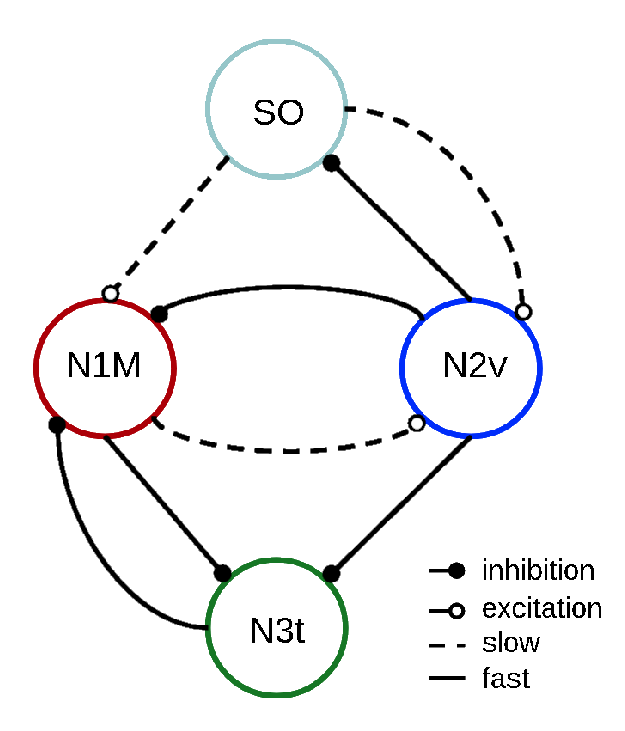
\includegraphics[width=\textwidth]{methods/invariants-model/figure1b.eps}
	\end{minipage}
	\caption{\textbf{Panel (a)}. Ionic channel distribution in the two-compartment description for the individual neurons in the Vavoulis et al. model used in this study. At the soma: $I_{ACh}$, acetylcholine ionic channel; $I_{NaL}$, slowly inactivating sodium
		ionic channel;$I_T$, low-threshold calcium current; $I_{inj}$, injected current; $I_{L,S}$, leakage current in the soma; $I_{syn}$, synaptic current. At the axon: $I_{NaT}$, fast inactivating sodium current; $I_K$, delayed rectifier potassium current; $I_{L,A}$, leakage current in the axon. The color for each $I_X$ current represents the CPG neuron that includes it at the soma,  N1M, N2v and N3t, respectively. \textbf{Panel (b)}. Connection scheme for the {\sl Lymnaea} feeding CPG circuit model. The colors indicating each neuron in the circuit match those in the representation of their corresponding somatic membrane potential traces in section \ref{sec:CPG model}. 
	}
	\label{fig:CPG diagram 2 compartments}
\end{figure}

\begin{figure}[htb!]
	\centering
	\includegraphics[width=0.7\linewidth]{methods/invariants-model/figure2.eps}
	\caption{Triphasic feeding rhythm as produced by the circuit CPG model described in Fig. \ref{fig:CPG diagram 2 compartments}. In this simulation, $i_{inj}$ values applied to each neuron are 8.5, 6, 2 and 0 mV, respectively.}
	\label{fig:model simulation}
\end{figure}



\subsection{CGC neuron model}
This model is described by six different ionic channels: Persistent and transient sodium currents ($I_{NaP}$, $I_{NaT}$), that primarily drive depolarization and action potential initiation; transient and delayed rectifier potassium currents ($I_A$, $I_D$), key for repolarization and contribute to the shoulder shape waveform in this neuron (specially $I_D$); and a low-voltage-activated and high-voltage-activated calcium currents ($I_{LVA}$, $I_{HVA}$), which are crucial for both immediate excitability and long-term plasticity. These channels are described by Eqs. \ref{eq:voltage} to \ref{eq:channels}. 

\begin{equation}
C_m\frac{dV}{dt} = I_{inj} - I_{NaT} - I_{NaP} - I_{A} - I_{D} - I_{LVA} - I_{HVA},
\label{eq:voltage}
\end{equation}

\begin{equation}
I_{NaT} = g_{NaT} m_{{\infty}}^3 h (V - E_{Na}),
\end{equation}
\begin{equation}
I_{NaP} = g_{NaP} r^3 (V - E_{Na}),
\end{equation}
\begin{equation}
I_{A} = g_{A} a^4 b (V - E_{K}),
\end{equation}
\begin{equation}
I_{D} = g_{D} n^4 (V - E_{K}),
% \label{eq:channels}
\end{equation}
\begin{equation}
I_{LVA} = g_{LVA} c_{{\infty}}^3 d_{{\infty}} (V - E_{Ca}),
\end{equation}
\begin{equation}
I_{HVA} = g_{HVA} e^3 f (V - E_{Ca}).
\label{eq:channels}
\end{equation}

Inactivation and activation dynamic variables $r,a,n,e$ and $h,b,f$ are defined by:
\begin{equation}
\frac{dx}{dt} = \frac{x_{\infty}-x}{\tau_x},
\end{equation}
where $x = h,r,a,b,n,e$ or $f$ and $x_{\infty}$ and $tau_x$ are defined by:

\begin{equation}
x_{\infty} = {(1+exp(\frac{V_H^x-V}{V_S^x}))}^{-1}
\end{equation}

See Supplementary Material in \cite{vavoulis_balanced_2010} for more details. 

The implementation of this model is available at Neun library \href{https://github.com/GNB-UAM/neun}{github.com/GNB-UAM/neun} (VavoulisCGCModel).

\begin{figure}[htb!]
	\centering
	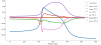
\includegraphics[width=\textwidth]{img/laser/cgc-model-simulation.pdf}
	\caption{Simulation of the CGC-model representing the voltage dynamics during an action potential and the corresponding ionic currents defined in the model ($I_{\textrm{NaP}}$,$I_{\textrm{NaT}}$, $I_{\textrm{A}}$, $I_{\textrm{D}}$, $I_{\textrm{LVA}}$,$I_{\textrm{HVA}}$). The units in the $y$-axis are specified in the legend.}
	\label{fig:model cgc currents}
\end{figure}


\subsubsection{Temperature dependence description in the model}
\label{sec:model equations temperature}
To simulate the temperature dependency in the neuronal activity, a $Q_{10}$ factor was incorporated to every dynamical equation in the model (i.e., conductances and activation gates). $Q_{10}$ represents temperature sensitivity in each channel and it was included as a new factor as shown in Eqs. \ref{Q10_conductance} and \ref{Q10_gates}, with $i=Na_T,Na_P,A,D,LVA,HVA$ for Eq. \ref{Q10_conductance} and $i=h,r,a,b,n,d,e,f$ for Eq. \ref{Q10_gates}. The capacitance was also defined as temperature dependent ($C_T$) with a linear relation to the difference of temperature: 

\begin{equation}g_i(T)=\bar{g}_i{Q^i_{10}}^{\frac{T-T_0}{10}},
\label{Q10_conductance}
\end{equation}
\begin{equation}\phi_i(T)=\bar{\phi}_i{Q^i_{10}}^{\frac{T-T_0}{10}},
\label{Q10_gates}\end{equation}
\begin{equation}C_T=c_0 + c_0 \gamma(T-T_0).\end{equation}


where $\bar{g}_i$, $\bar{\phi}_i$, $c_0$ are the original values used in the model and $\gamma = 0.05$.

 
\section{Neural data analysis}
%Detectar eventos --> secuencia
% Eventos promediados ocultan información --> secuencialidad ciclo a ciclo
%Métricas

To analyze the recordings of intracellular signals and the outputs of the models simulations, we relied on the detection of single events, mainly spikes and then we either defined time-intervals for the CPG rhythm or analyze each single spike based on metrics as in chapter \ref{c-laser}. The detection of these references allowed us to study the sequentiality of neural dynamics at different time-scales. Also, we focused on each event and cycle, avoiding the averaging of the results, since we consider this hinders information in the activity, such as the sequential activation cycle-by-cycle. 

For the study of the time-intervals variability and the presence os sequential dynamical invariants, the spikes of the recordings and model simulation of the bursting activity were detected using the change in the derivative along with a voltage threshold condition, i.e., all peaks over a voltage value were considered action potential peaks. Then, bursts were identified from the temporal structure of the spikes, and intervals were characterized by the timing of the first and last spike in each burst. In some recordings this temporal reference was adjusted to the needs of the data available, this will be specified in the corresponding section \ref{sec:experimental sussex}.

All intervals defined in section \ref{subsec:intervals} were defined by the events in the ini and end of the burst, the time-intervals described were characterized as follows:

%For the boxplots, the Python library matplotlib.pyplot used each cycle-by-cycle interval duration. Linear regression from sklearn Python library was used to quantify the relation of the sequence intervals to the instantaneous period of each cycle. 

\begin{lstlisting}
	#########  SINGLE INTERVALS
	# on = 0; off = 1
	
	# off1 - on1
	def get_burst_duration(data):
		return np.array([b - a for a, b in zip(data[:, 0], data[:, 1])])
	
	# on2 - off1
	def get_burst_interval(data):
		return np.array([a - b for a, b in zip(data[1:, 0], data[:, 1])])
		
	# on2 - on1
	def get_burst_period(data):
		return np.array([a - b for a, b in zip(data[1:, 0], data[:, 0])])
		
	#########  PAIRED INTERVALS
	def get_intervals(d1,d2):
		if d1.size == 0 or d2.size == 0:
			return [],[]
			
		d1d2_interval = np.array([b-a for a,b in zip(d1[:,0],d2[:,0])])
		d1d2_delay = np.array([b-a for a,b in zip(d1[:,1],d2[:,0])])
		d2d1_interval = np.array([a-b for a,b in zip(d1[1:,0],d2[:-1,0])])
		d2d1_delay = np.array([a-b for a,b in zip(d1[1:,0],d2[:-1,1])])
	
		return [d1d2_interval,d1d2_delay],[d2d1_interval,d2d1_delay]
\end{lstlisting}

On the other hand, in the recordings and model simulations of the tonic firing activity of large cells in the right parietal ganglia, regarding the stereotyped spike waveform it was enough with a voltage threshold to detect the events in the sequence, and to analyze the waveoform after the detection of the events, each one was extended N milliseconds left and right, defining segments of signal that capture the shape of the waveform. The characterization of that waveform was carried by defining four metrics: the duration, amplitude and depolarization and repolarization slopes, implemented as follows:

\begin{lstlisting}
def get_spike_duration(spike,dt,tol=2, thres_val=0.5, max_dur = 5, v_scale=1): 
	spike = spike[~np.isnan(spike)]
	
	peaks, properties = find_peaks(spike, prominence=1*v_scale, width=20)
	
	#Warning: this may fail for not centered waveforms	
	if len(peaks)>1: # in case spike has several peaks, gets mid one.
		mid_peak = np.isclose(len(spike)//2, peaks, atol=10)
		peaks = peaks[mid_peak]
	results_half = peak_widths(spike, peaks, rel_height=thres_val)
	
	try: 
		duration_vals = np.array([results_half[2][0], results_half[3][0]])
		th = results_half[1]
	except Exception as e:
		duration_vals = np.array([])
		th = 0
	
	if duration_vals.size == 0: #Safety comprobation
		return (0,0),th
	else:
		return (duration_vals[0]*dt,duration_vals[-1]*dt),th
	
def get_spike_duration_value(waveform, dt, plot=False, v_scale=1):
	dur_refs,th = get_spike_duration(waveform, dt, plot=plot, v_scale=v_scale)
	duration = dur_refs[1]-dur_refs[0]
	return duration

# Description: 
# 	Recives spike values and return the amplitude value measured as the distance between
#	maximum and minimum voltage value.
# Parameters:
# 	spike voltage values
# 	dt time rate
# Return:
#	amplitude
def get_spike_amplitude(spike,dt, v_scale=1):
	spike = spike[~np.isnan(spike)] 
	mx_value = np.max(spike) #maximum V value (spike)
	mn_value = np.min(spike) #minimum V value (spike)

	return mx_value-mn_value

# Description: 
# 	Recives spike values and return the increasing and decreasing slope values at the 
#	two points matching a threshold in "the middle" of the spike maximum and minimum voltage value.
# Parameters:
# 	spike voltage values
# 	dt time rate
# 	n_points: number of points around position to calculate slope
#   slope_position: where to calculate slope: defalult value, mid of spike.
# Return:
#	depolarization slope, repolarization slope 

def get_slope(spike,dt,n_points=10, slope_position=0.5, plot=False, v_scale=1):
	spike = spike[~np.isnan(spike)] 
	mid_ps,th = get_spike_duration(spike,dt,thres_val=slope_position, v_scale=v_scale)
	indx1 = int(mid_ps[0]/dt) #From ms to point ref
	indx2 = int(mid_ps[1]/dt) #From ms to point ref
	
	scale = int(0.1/dt)
	n_points *= scale
	
	n_ms = n_points*dt
	
	slope1 = (spike[indx1+n_points]-spike[indx1-n_points])/(n_ms*2) 
	slope2 = (spike[indx2+n_points]-spike[indx2-n_points])/(n_ms*2)

	return (slope1,slope2)
\end{lstlisting}

Finally, model were implemented in $C++$ taking advantage of its computational speed and most analysis where performed in Python3, since it is a frequently used tool and libraries such as Pandas are very effective for data analysis. Scripts used in this work are available at \href{https://github.com/agarpe/neural-dynamics-utils}{github.com/agarpe/neural-dynamics-utils} and all conductance-based models are included in Neun \href{https://github.com/agarpe/neural-dynamics-utils}{github.com/agarpe/neural-dynamics-utils}


\section{CW-NIR laser}
The experimental results presented here were obtained using a continuous-wave (CW) NIR diode laser in single TEM00 operation and 830nm wavelength output (Integrated Optics 0830L-13A-NI-PT-NF). \begin{wrapfigure}{l}{0.5\textwidth}
    \centering
	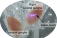
\includegraphics{img/laser/laser-beam.pdf}
	\caption{Illustration of the laser beam focused on a neuron in the right parietal ganglia.}
	\label{fig:laser beam}
\end{wrapfigure} 
In Figure \ref{fig:laser setup} shows the experimental setup. The diode laser output was coupled to a single-mode optical fiber to efficiently guide the laser beam to the sample. To adapt the divergence of the laser beam to the fiber optic output, an aspherical lenses-collimator (Thorlabs, F280FC-850) was installed. An achromatic doublet with focal length f=50mm was used to focus the laser beam on the sample (Thorlabs AC127-050-B-ML). The experiments were performed with a laser output power of $\sim$ 90 mW and a power density over the sample of 146 W/cm². The grazing incidence of the laser beam on the sample created a quasi-elliptical spot, with a minor axis of approximately 34{\textmu}m, as shown in Fig. \ref{fig:laser beam}.

The laser was attached to a micro-manipulator (Siskiyou MX160), allowing micrometer precision of the beam placement over the neuron and optimization of the beam focus. The focusing was performed using a binocular microscope (Nikon SMZ-1500) coupled to a CCD camera (XCAM1080PHA, ToupTek Photonics, Zhejiang, China).

\begin{figure}[htb!]
	\centering
	\includegraphics[width=0.7\textwidth]{img/methods/laser-setup_labels.png}
	\caption{Image of the NIR-laser stimulation setup. On the left there is the micromanipulator with the electrode and the glass micropipette for the intracellular recording. In the center of the image in the base there is the preparation of the CNS of \textit{Lymnaea stagnalis}. On the right side the laser fiber is attached to the collimator and at the end of the holder there is the lenses to focus the laser beam. This is also attached to another micromanipulator for a precise focusing.}
\end{figure}


\section{Temperature estimation for analyzing laser neuromodulation}
\label{sec:temperature-estimation}
To estimate the CW-NIR laser induced temperature change, we used the open-pipette method employed in previous experimental studies to measure the temperature variation during the illumination \parencite{li_temporal_2013, rabbitt_heat_2016,brown_thermal_2020, brown_response_2021}. We calibrated the resistance and temperature relation using a thermistor (EPCOS, 10$k\Omega$) to measure the temperature in the preparation solution in the range from 23ºC to 29ºC. We used two protocols:  injecting a constant current to calculate the resistance change from the voltage recording, and injecting pulses of a specific current value. From the resulting recording slope of the linear regression, we computed the conversion from voltage to temperature. For the estimation of the temperature change during the laser stimulation, we measured the voltage change during short intervals of laser illumination and the temperature value at its saturation plateau. This estimation is represented in Fig. \ref{fig:temperature estimation}.



\begin{figure}[htb!]
	\centering
	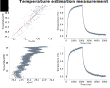
\includegraphics[width=0.8\textwidth]{img/laser/temperature_estimation.pdf}
	\caption{Open-pipette temperature estimation method. Each row in the panel represents pulsed and continuous current delivery for the estimation, respectively. For both examples: left column, temperature and voltage relation. Right column filtered mean of voltage recordings from short illumination intervals in the pipette. }
	\label{fig:temperature estimation}
\end{figure}


\chapter{Sequential constrains in CPG circuits: Dynamical invariants}
\label{c-invariants}
\section{Introduction}
\section{Methods}
\section{Dynamical invariant in computational models}
The first objective reported in this section was to reproduce in a computational model the cycle-by-cycle sequential restrictions found in \cite{elices_robust_2019}. For that we used the feeding CPG model description of \cite{vavoulis_dynamic_2007}, that does not have a chaotic mode, but the model is flexible enough to adapt the variability of one of the neurons. Following the current injection protocol defined in section \ref{subsec:inj protocol}, N1M, N3t and SO neurons in the model were stimulated for our analysis of the sequence interval variability. Using this induced variability we were able to explore the presence of sequential dynamical invariants under different scenarios. The effect on injecting a current ramp on N2v is not reported here since it leads to lower variability than the other cases. In all simulations, we could test the robustness of the rhythm while inducing the external perturbation that evoked variability in the search for dynamical invariants. The results summarized and adapted for this section were published in \cite{garrido-pena_characterization_2021}.

First result we report is that the the model of the feeding CPG faithfully reproduces the activity of the main neurons involved in the generation of its triphasic rhythm \parencite{vavoulis_dynamical_2007}. This includes their waveforms and the relationships between the cycle period and the duration of several intervals reported in \parencite{elliott_temporal_1991}. Note that, since there was not a description of a chaotic mode, all the rhythms explored here were analyzed from induced stimulation, not by simulating spontaneous activity. This was a restriction when exploring spontaneous activity, since the circuit needed to be altered by one of the neurons, simulating a extended experimental protocol, but still altering the circuit in a predefined way. Also, other phenomena reported in the pyloric CPG experimental work, were there was a "reset" in the inter-cycle dynamics of the dynamical invariants, could not be explored in this model, since the ramp value was progressive (see Apendix Fig. \ref{fig:N1M stimulation pairplot reset} for a representation of this non-reset output). All this will be reported in the following Section \ref{sec:experimental sussex} with experimental recordings and other options to reproduce the functional variability will be discussed in Sec. \ref{sec:model variability}

\subsection{N1M driven variability}
\label{subsec:n1m driven}

N1M neuron is frequently stimulated using ramp protocols in living preparations \parencite{elliott_temporal_1991} as it plays an important role in initiating the CPG rhythm. In our case, after applying the current injection protocol into N1M and detecting the spike and burst events for each neuron in the CPG model, all  intervals represented in Fig. \ref{fig:intervals} were quantified. We show in Fig. \ref{fig:invariant n1m} the variability and the correlation between the period and each interval.

Figure \ref{fig:invariant n1m}.a. displays the boxplots of the duration of all sequence intervals defined above. Regarding burst duration of the neurons (N1M-BD, N2v-BD, N3t-BD), we can observe in this figure that the most variable one corresponds to N3t neuron. Furthermore, the derived intervals which cover N3 burst duration are also the ones presenting larger variability (i.e., N2-N1, N3-N1 and N3-N2 intervals and N2-N1 delay). On the other hand, the least variable intervals correspond to the ones related to N2v and N1M burst duration, i.e., N1-N2, N1-N3, N2-N3 intervals and N1-N2, N1-N3, N3-N1, N2-N3, N3-N2 delays. They show a nearly a constant duration during each period.

Figure \ref{fig:invariant n1m}.b. plots the cycle-by-cycle measurements of the intervals defined in \ref{fig:intervals} against the period. The first row displays burst duration intervals, which are the intervals analyzed in Elliot et al. \parencite{elliott_temporal_1991} from data obtained in electrophysiological recordings of living neurons, and in Vavoulis et al. from data obtained in model simulations \parencite{vavoulis_computational_2007}. The results shown in this row match those results, being N3t-BD the most correlated to the period, which can be noted by the $R^2$ value close to one in the linear regression. The other two intervals (N1M-BD and N2v-BD), which were also the least variable, are not strongly correlated to the period. 

Likewise, the most variable intervals derived from other time references of the sequence also show a high correlation with the period, i.e., they present dynamical invariants, in this case N2-N1, N3-N1, N3-N2 intervals and N2-N1 delay. The cycle-by-cycle period variability is a consequence of the variability in these specific intervals.

On the other hand, intervals related to neuron N2v and N1M are the least variable. N2v is the one least affected by the global activity of the circuit, in terms of its burst duration. Moreover, some of the intervals are very short, or even negative, since the end of a given neuron's burst overlaps the next one's beginning (N1-N2 and N3-N1 delay). This is the case for N1-N2 and N3-N1 delay (4th row, 1st column and 5th row, 1st column, respectively in Fig. \ref{fig:invariant n1m}.b.).  

%\begin{figure}[hbt!]
%	\begin{minipage}[b]{0.45\textwidth}
%		\centering
%		\includegraphics[width=\textwidth]{invariants/data/MODEL/n1m_driven/images/3phases/_boxplot.pdf}
%	\end{minipage}
%	\begin{minipage}[b]{0.53\textwidth}
%		\centering
%		\begin{minipage}[b]{\textwidth}
%			\centering
%			\includegraphics[width=\textwidth]{invariants/data/MODEL/n1m_driven/images/3phases/_durations.pdf}
%		\end{minipage}\
%		\begin{minipage}[b]{\textwidth}
%			\centering
%			\includegraphics[width=\textwidth]{invariants/data/MODEL/n1m_driven/images/3phases/_intervals.pdf}
%		\end{minipage}\
%		\begin{minipage}[b]{\textwidth}
%			\centering
%			\includegraphics[width=\textwidth]{invariants/data/MODEL/n1m_driven/images/3phases/_delays.pdf}
%		\end{minipage}
%	\end{minipage}
%	\caption{a).Box-plots of the  sequence intervals under N1M neuron stimulation. b) Interval correlations to period for N1M-driven simulation. First row: Burst duration. Second and third row: Two-neuron intervals. Forth and fifth row: Two-neuron delays. Linear relationships are quantified by the $R^2$ values of the regression.}
%	\label{fig:invariant n1m}
%\end{figure}





%
%\begin{figure}[h!]
%    \centering
%\includegraphics[width=\textwidth]{img/results-paper-modelo/figure5.eps}
%\caption{Box-plots of the  sequence intervals under N1M neuron stimulation.}
%\label{fig:invariant n1m boxplot}
%\end{figure}
%\clearpage
%\newpage
%\begin{figure}[h!]
%    \centering
%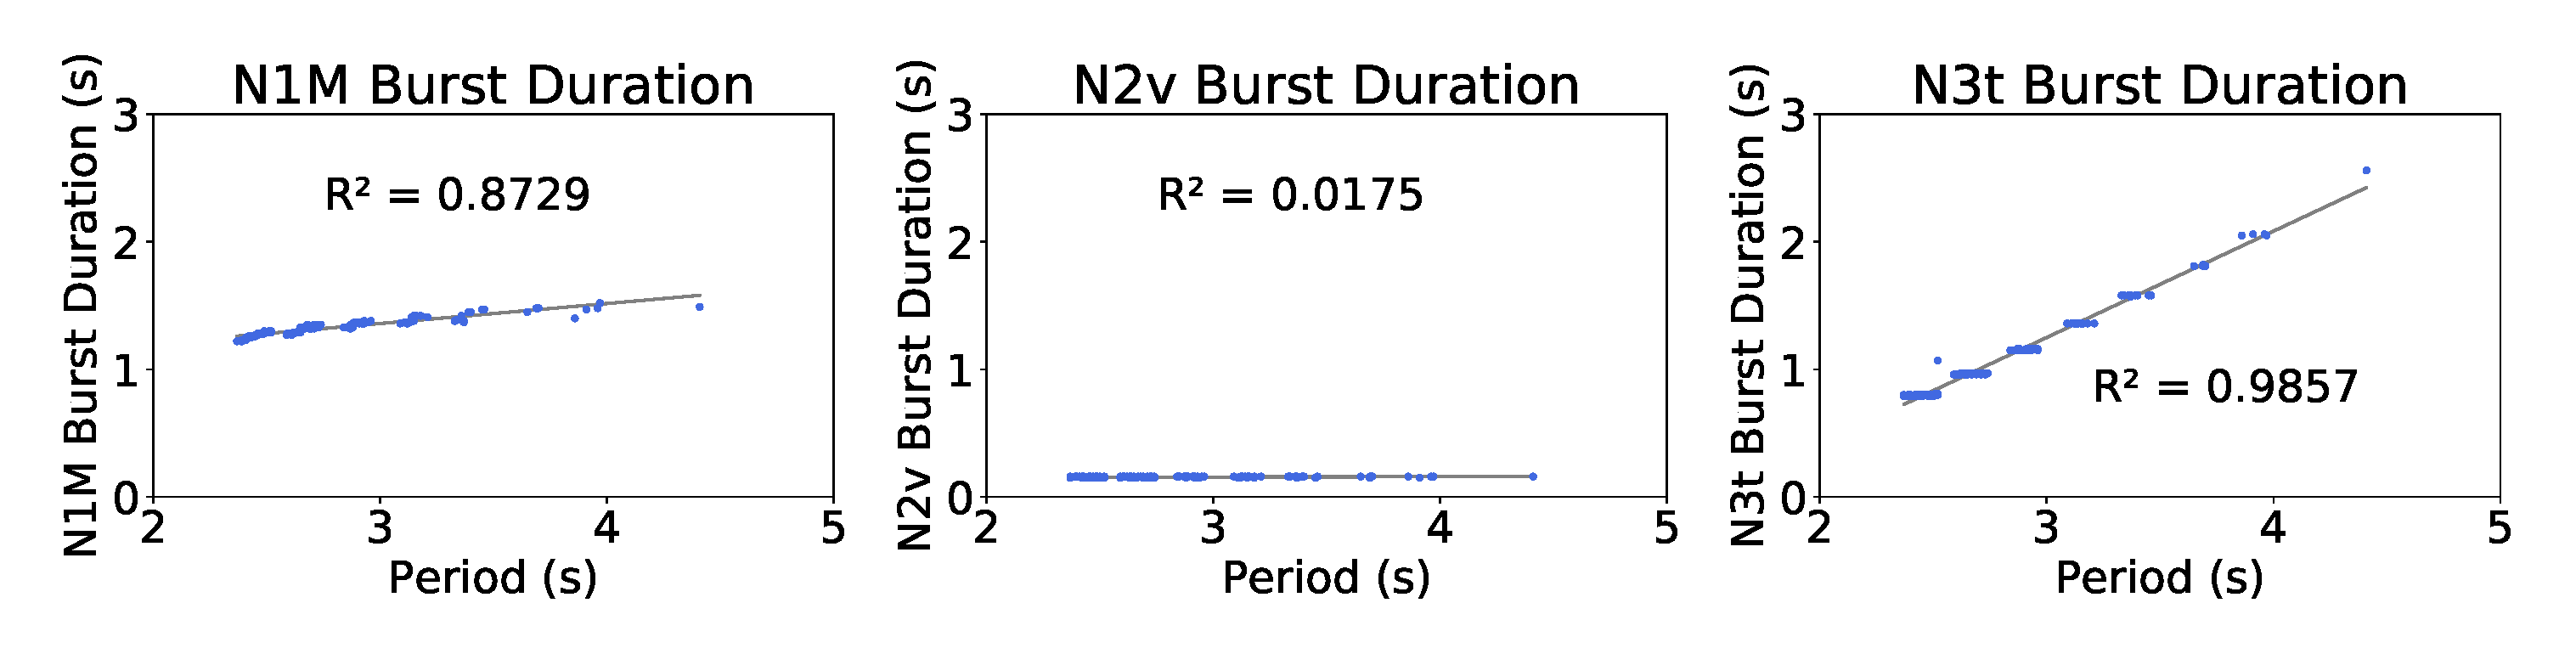
\includegraphics[width=\textwidth]{img/results-paper-modelo/figure6_row1.eps}
%  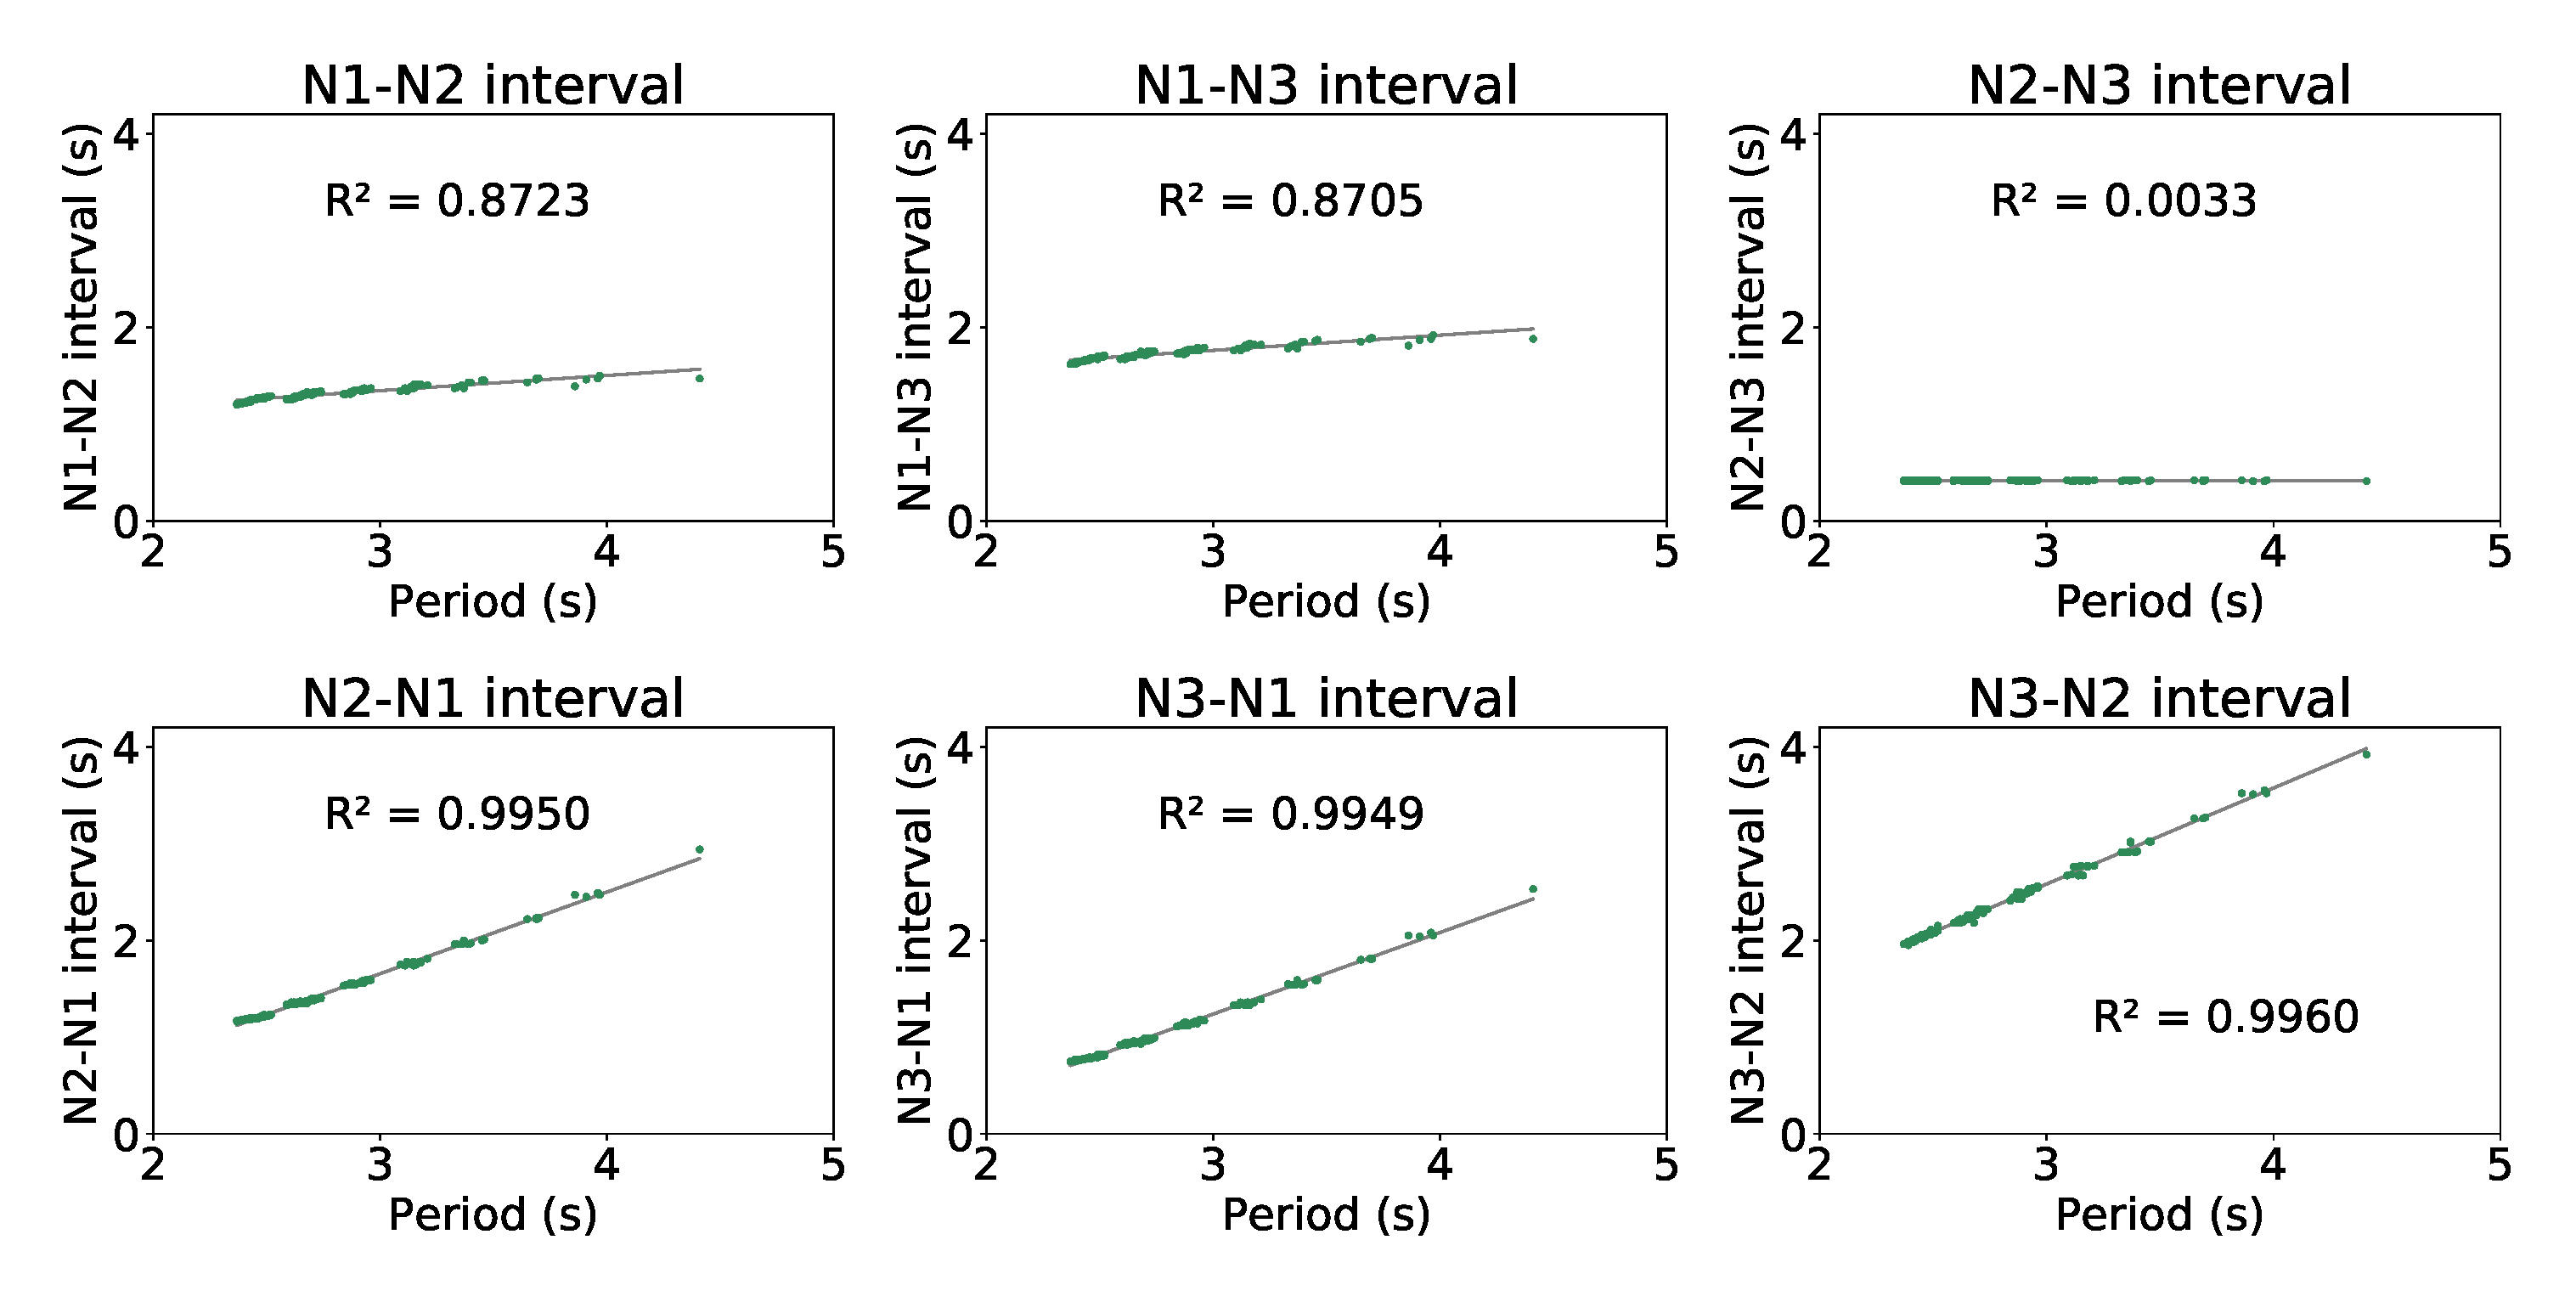
\includegraphics[width=\textwidth]{img/results-paper-modelo/figure6_row2-3.eps}%
%      
%  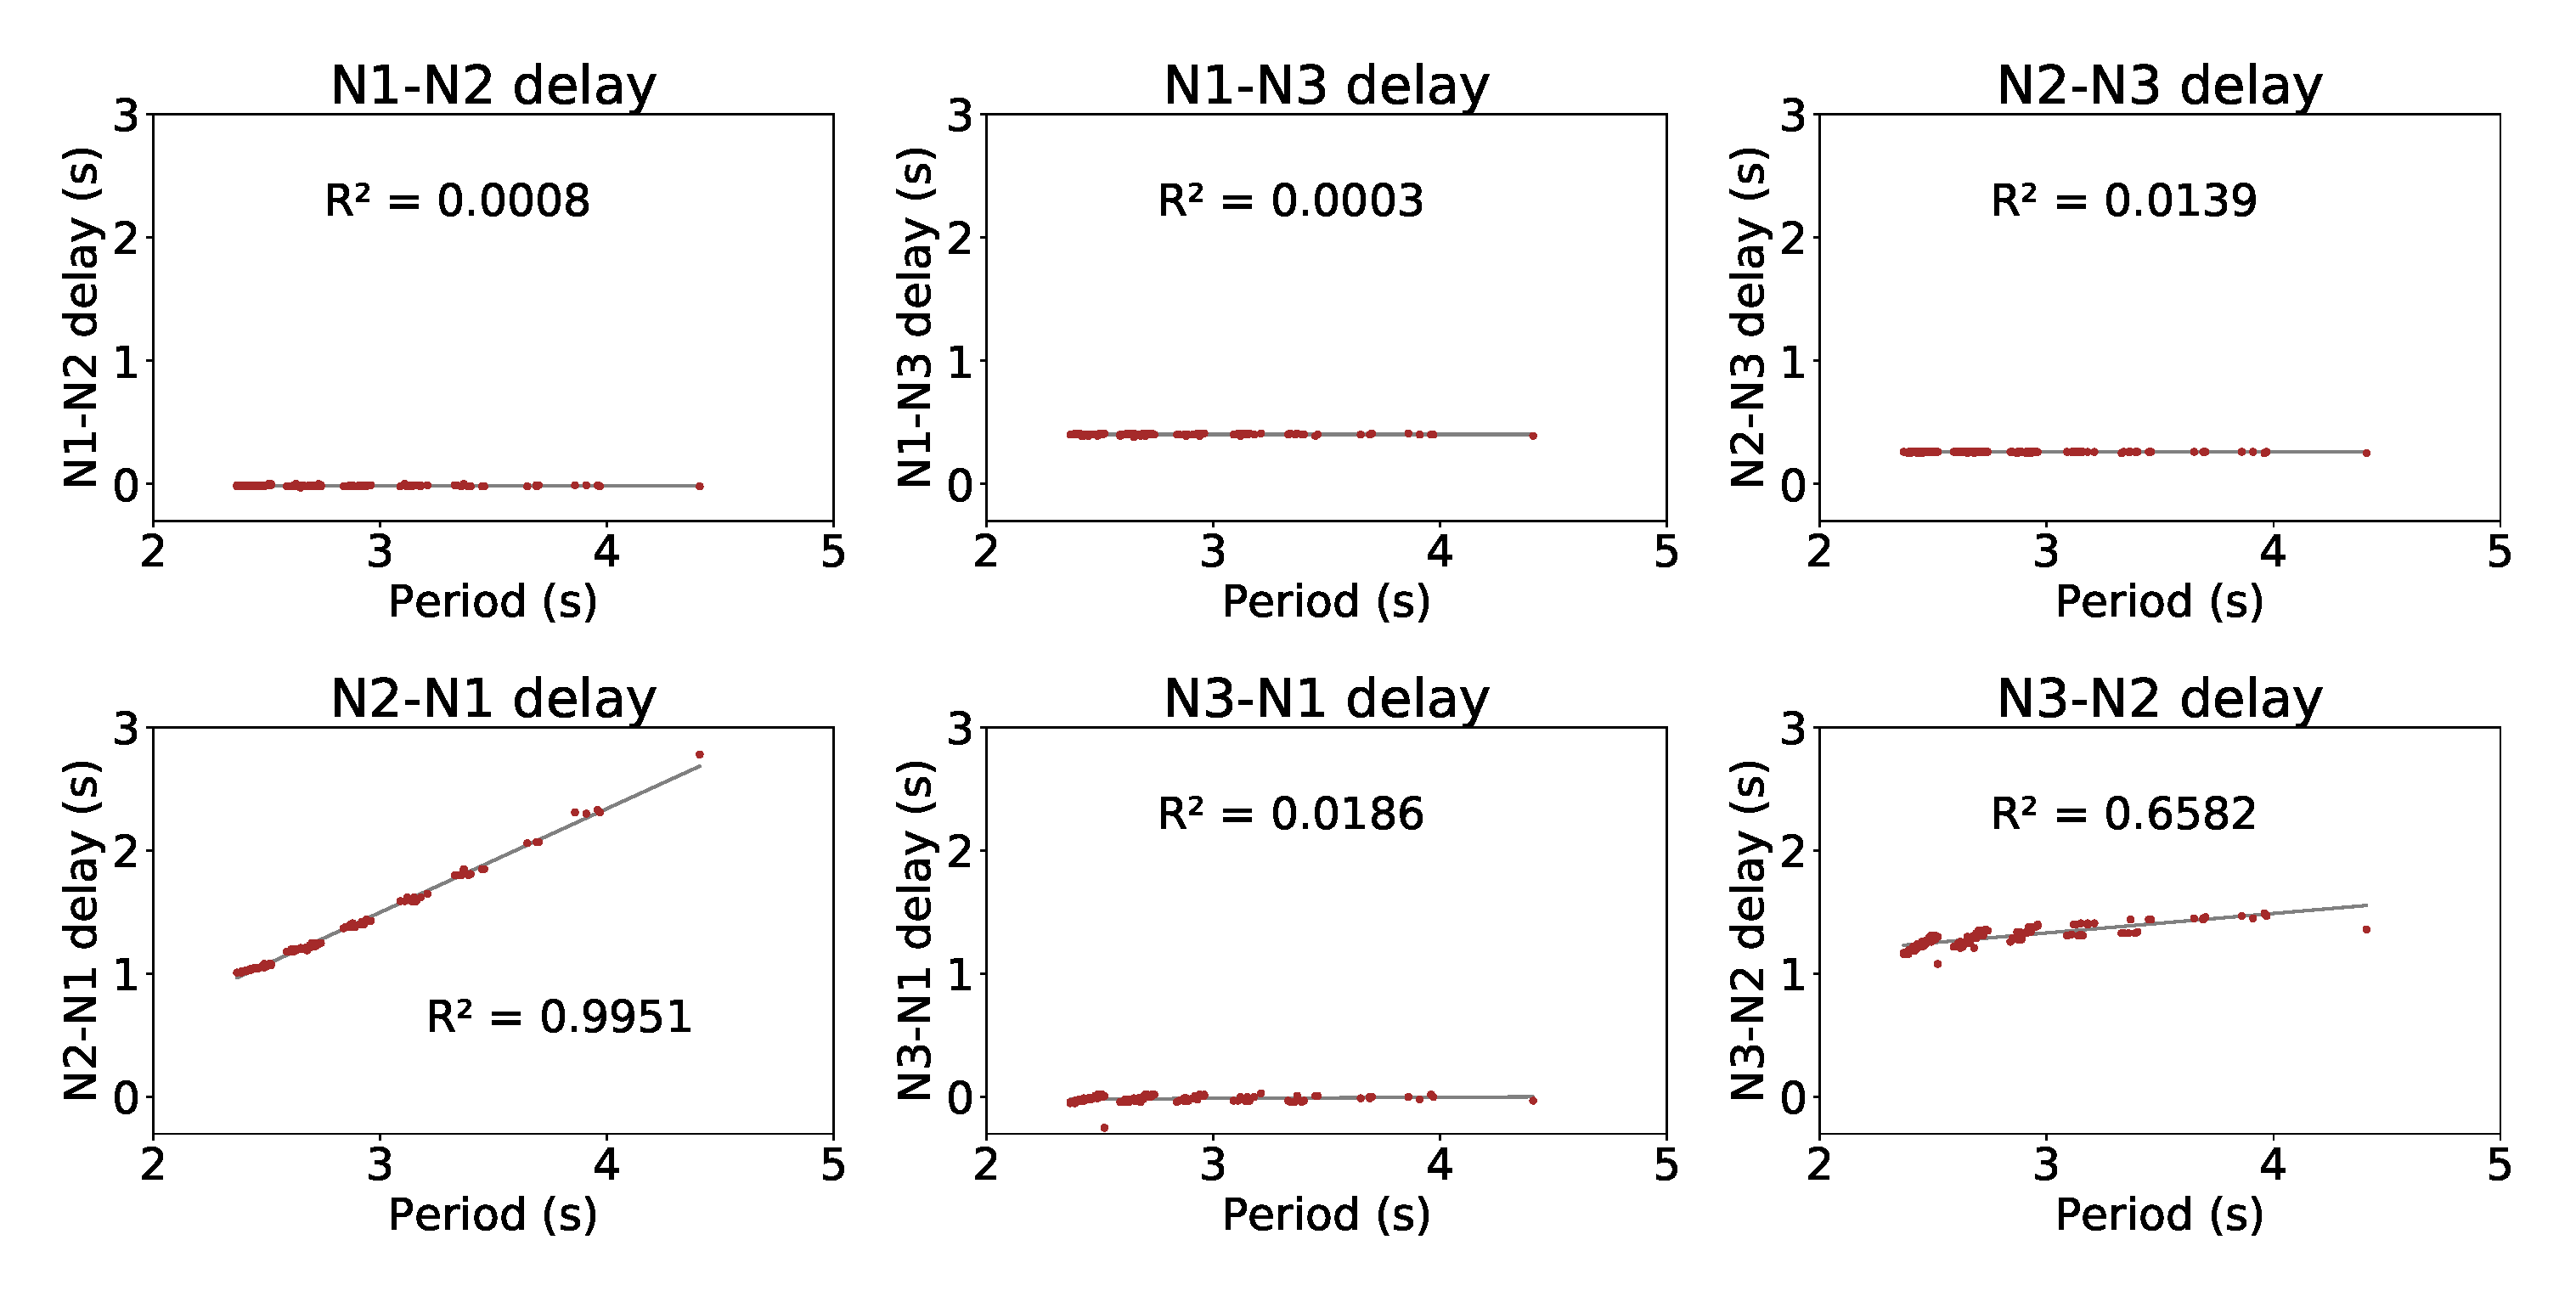
\includegraphics[width=\textwidth]{img/results-paper-modelo/figure6_row4-5.eps}%
%
%    \caption{Interval correlations to period for N1M-driven simulation. First row: Burst duration. Second and third row: Two-neuron intervals. Forth and fifth row: Two-neuron delays. Linear relationships are quantified by the $R^2$ values of the regression.}
%    \label{fig:invariant n1m}
%\end{figure}
%

\subsection{N3t driven variability}

The stimulation protocol was also applied to N3t neuron. In spite that no previous analysis on injecting a current ramp into this neuron has been reported neither experimentally nor in the feeding CPG computational model, due to the connectivity in the circuit, it can be expected that stimulation of N3t will induce variability in the rhythm. The characterization of the sequence intervals in this case are shown in Fig. 
\ref{fig:invariant n3t boxplot} and the correlation analysis is displayed in Fig. \ref{fig:invariant n3t test17}.
%In fact, we can expect a similar result to N1M-driven simulation because of their bidirectional connectivity see Fig. \ref{fig:CPG diagram}.  ***dicutir si es siméterica o no *****


Results shown in Fig. \ref{fig:invariant n3t boxplot} indicate that the larger variability is present in the same intervals related to N3t burst duration, as when the stimulation was delivered to N1M. However, in this simulation we observe that N1M had a lower variability while N3t had a higher variability with respect to the previous condition. 
%: N1M decreased its variability while N3t has increased it *****discutir***. 
In contrast, N2v-BD maintained its variability, as well as all the derived intervals containing this burst duration.

Note that N3-N1 delay, which is the interval from the end of the N3t burst to the beginning of N1M burst, shows negative values. This means that neuron N1M started earlier than the end of N3t in every cycle. Whilst this was also present in N1M-driven activity, here the variability of this interval is much higher, leading to a larger overlapping.
% N2v maintains its variability, being this interval and all the intervals related to it the least variable. Hence, in the distribution of the activity in the circuits between the neurons, the main negotiation is between N1M and N3t, distributing the variability and the period leading between they both. ***esto también lo tenemos que pulir un poco****

Figure \ref{fig:invariant n3t test17} plots each interval duration against the period. As in the previous condition, the dynamical invariants (i.e. intervals presenting a strong correlation to the period) show up in the intervals related to N3t, which were the ones presenting also the highest variability, whereas those intervals that do not participate in dynamical invariants, are the ones related to N1M and mostly N2v (the least variable ones). 


%The linear relationships regarding the least variable intervals (related to N2v and N1M burst durations), also present similar results to those discussed above when the rhythm was driven by N1M. Hence, the intervals most correlated are the ones with higher variability, whereas those intervals that do not participate in dynamical invariants, are the ones related to N1M and mostly N2v (the least variable ones).
%***revisar redundancia***
%
%\begin{figure}[h!]
%    \centering
%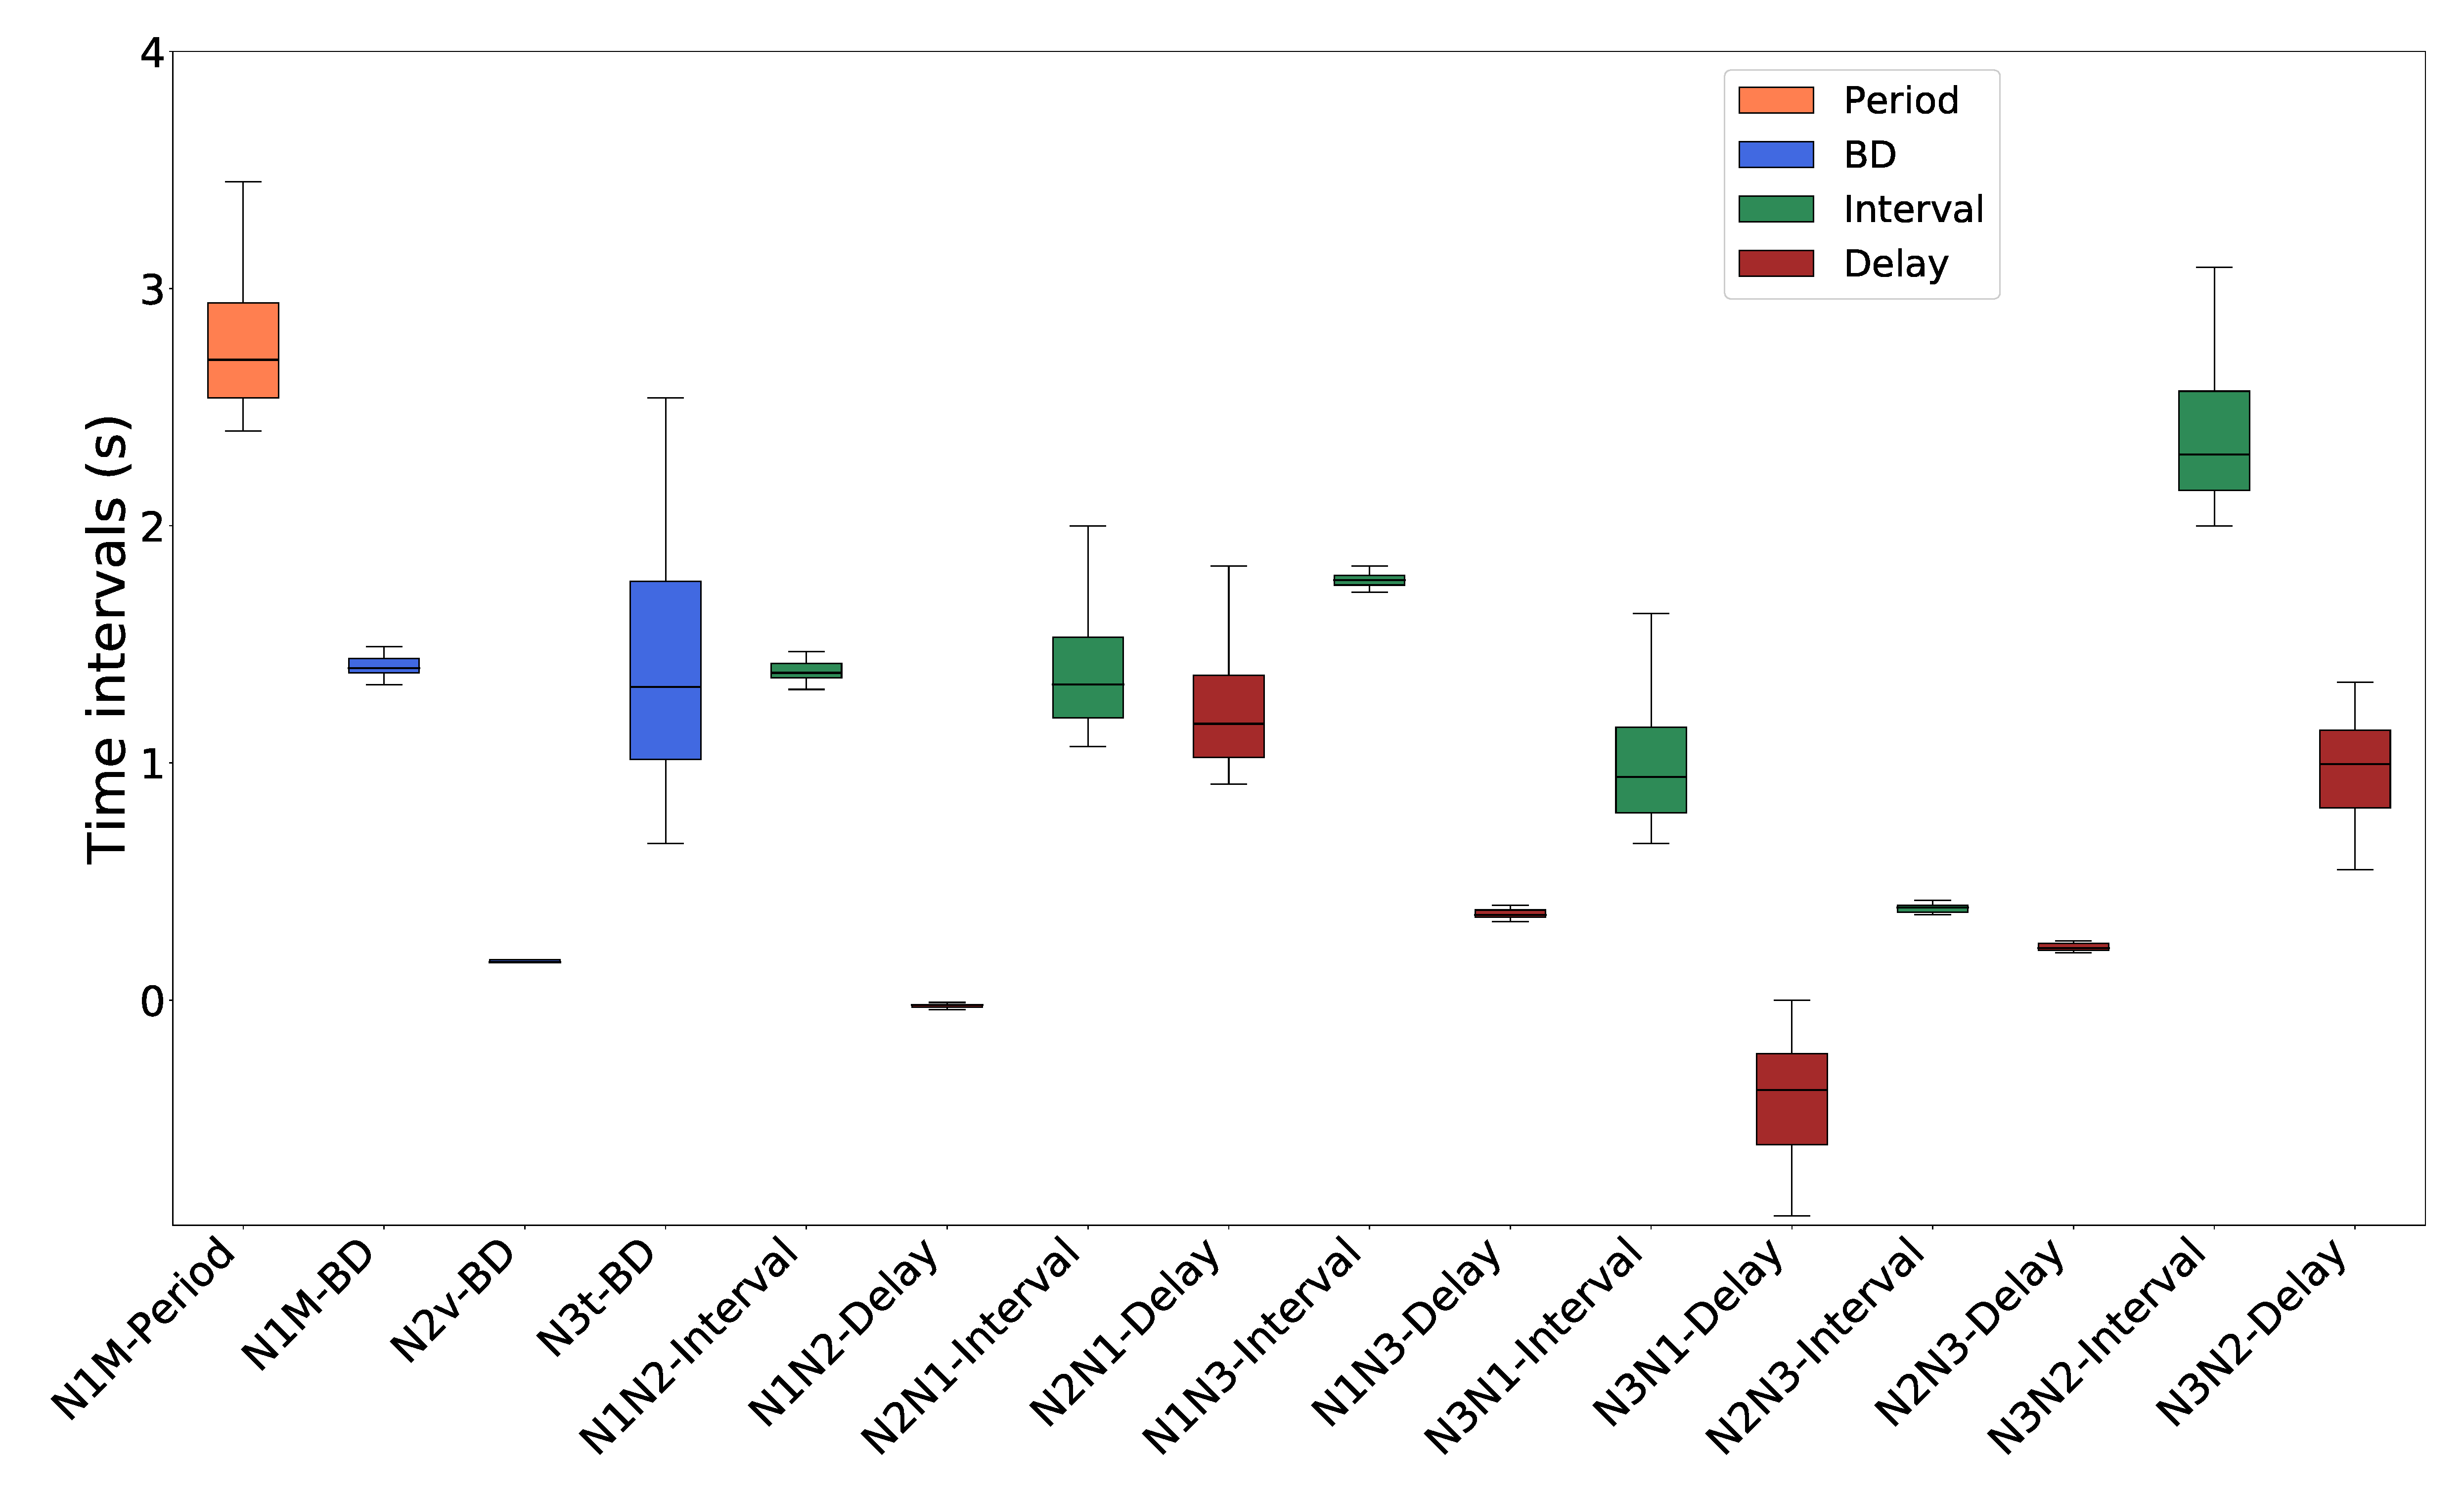
\includegraphics[width=\textwidth]{img/results-paper-modelo/figure7.eps}
%\caption{Box-plots of the sequence intervals under N3t neuron stimulation. }
%\label{fig:invariant n3t boxplot}
%\end{figure}

%
%\begin{figure}[h!]
%    \centering
%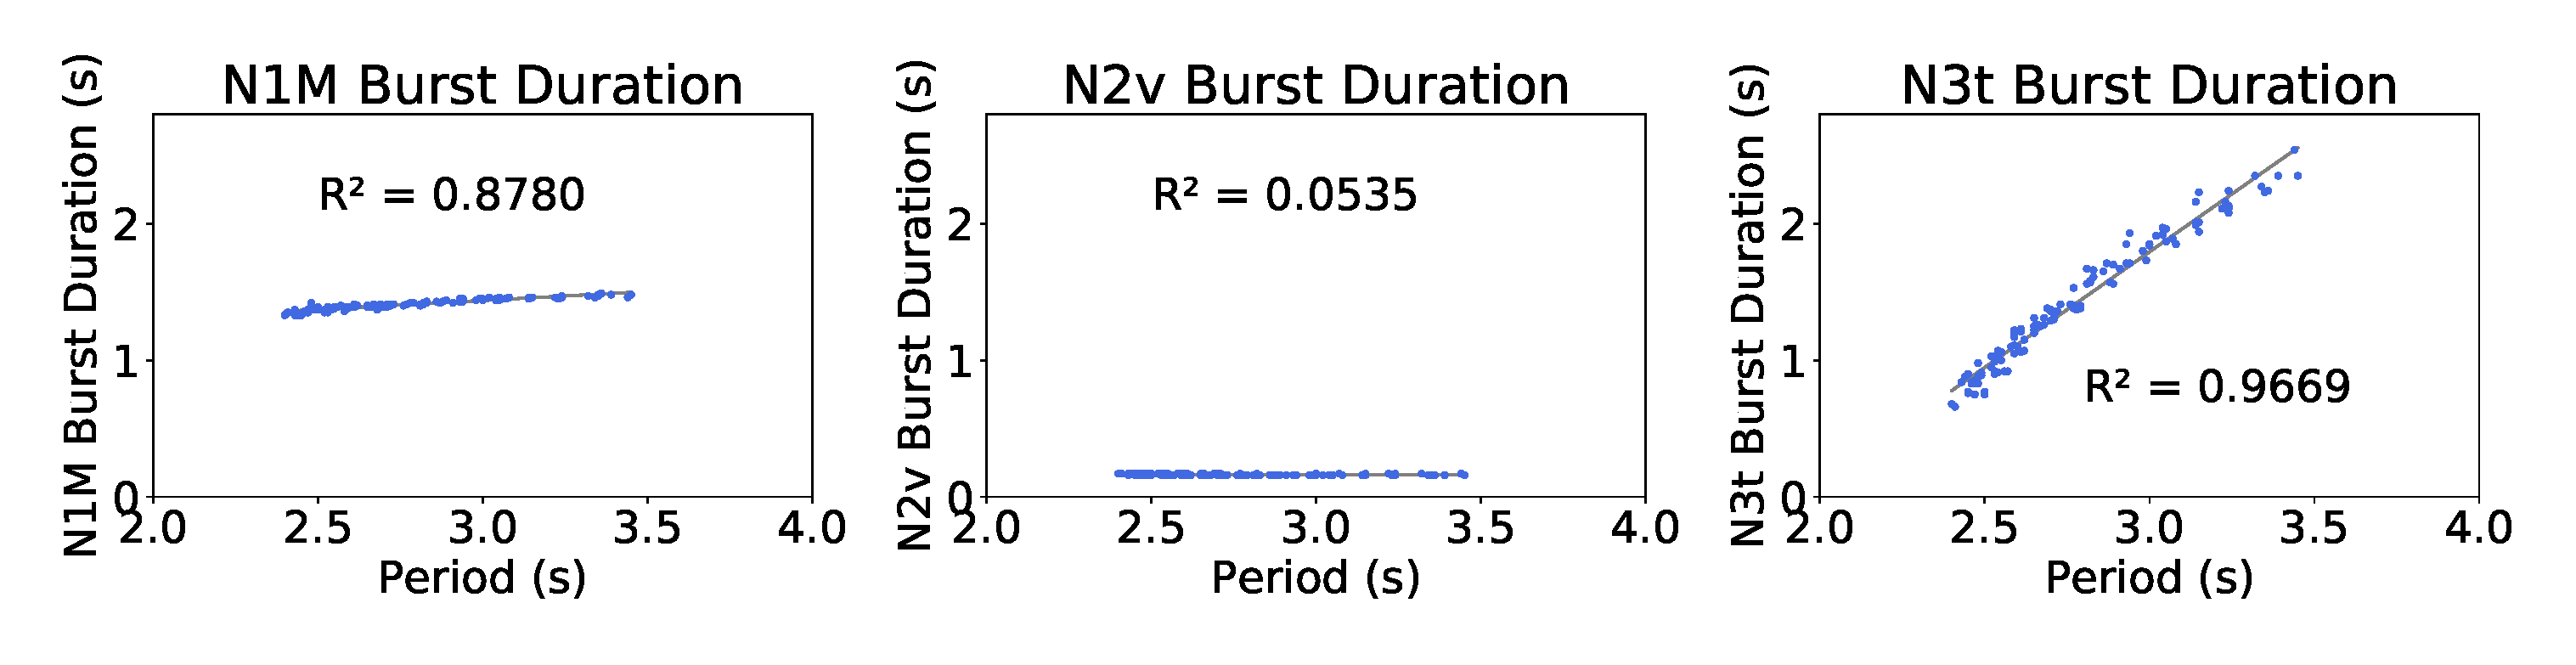
\includegraphics[width=\textwidth]{img/results-paper-modelo/figure8_row1.eps}
%  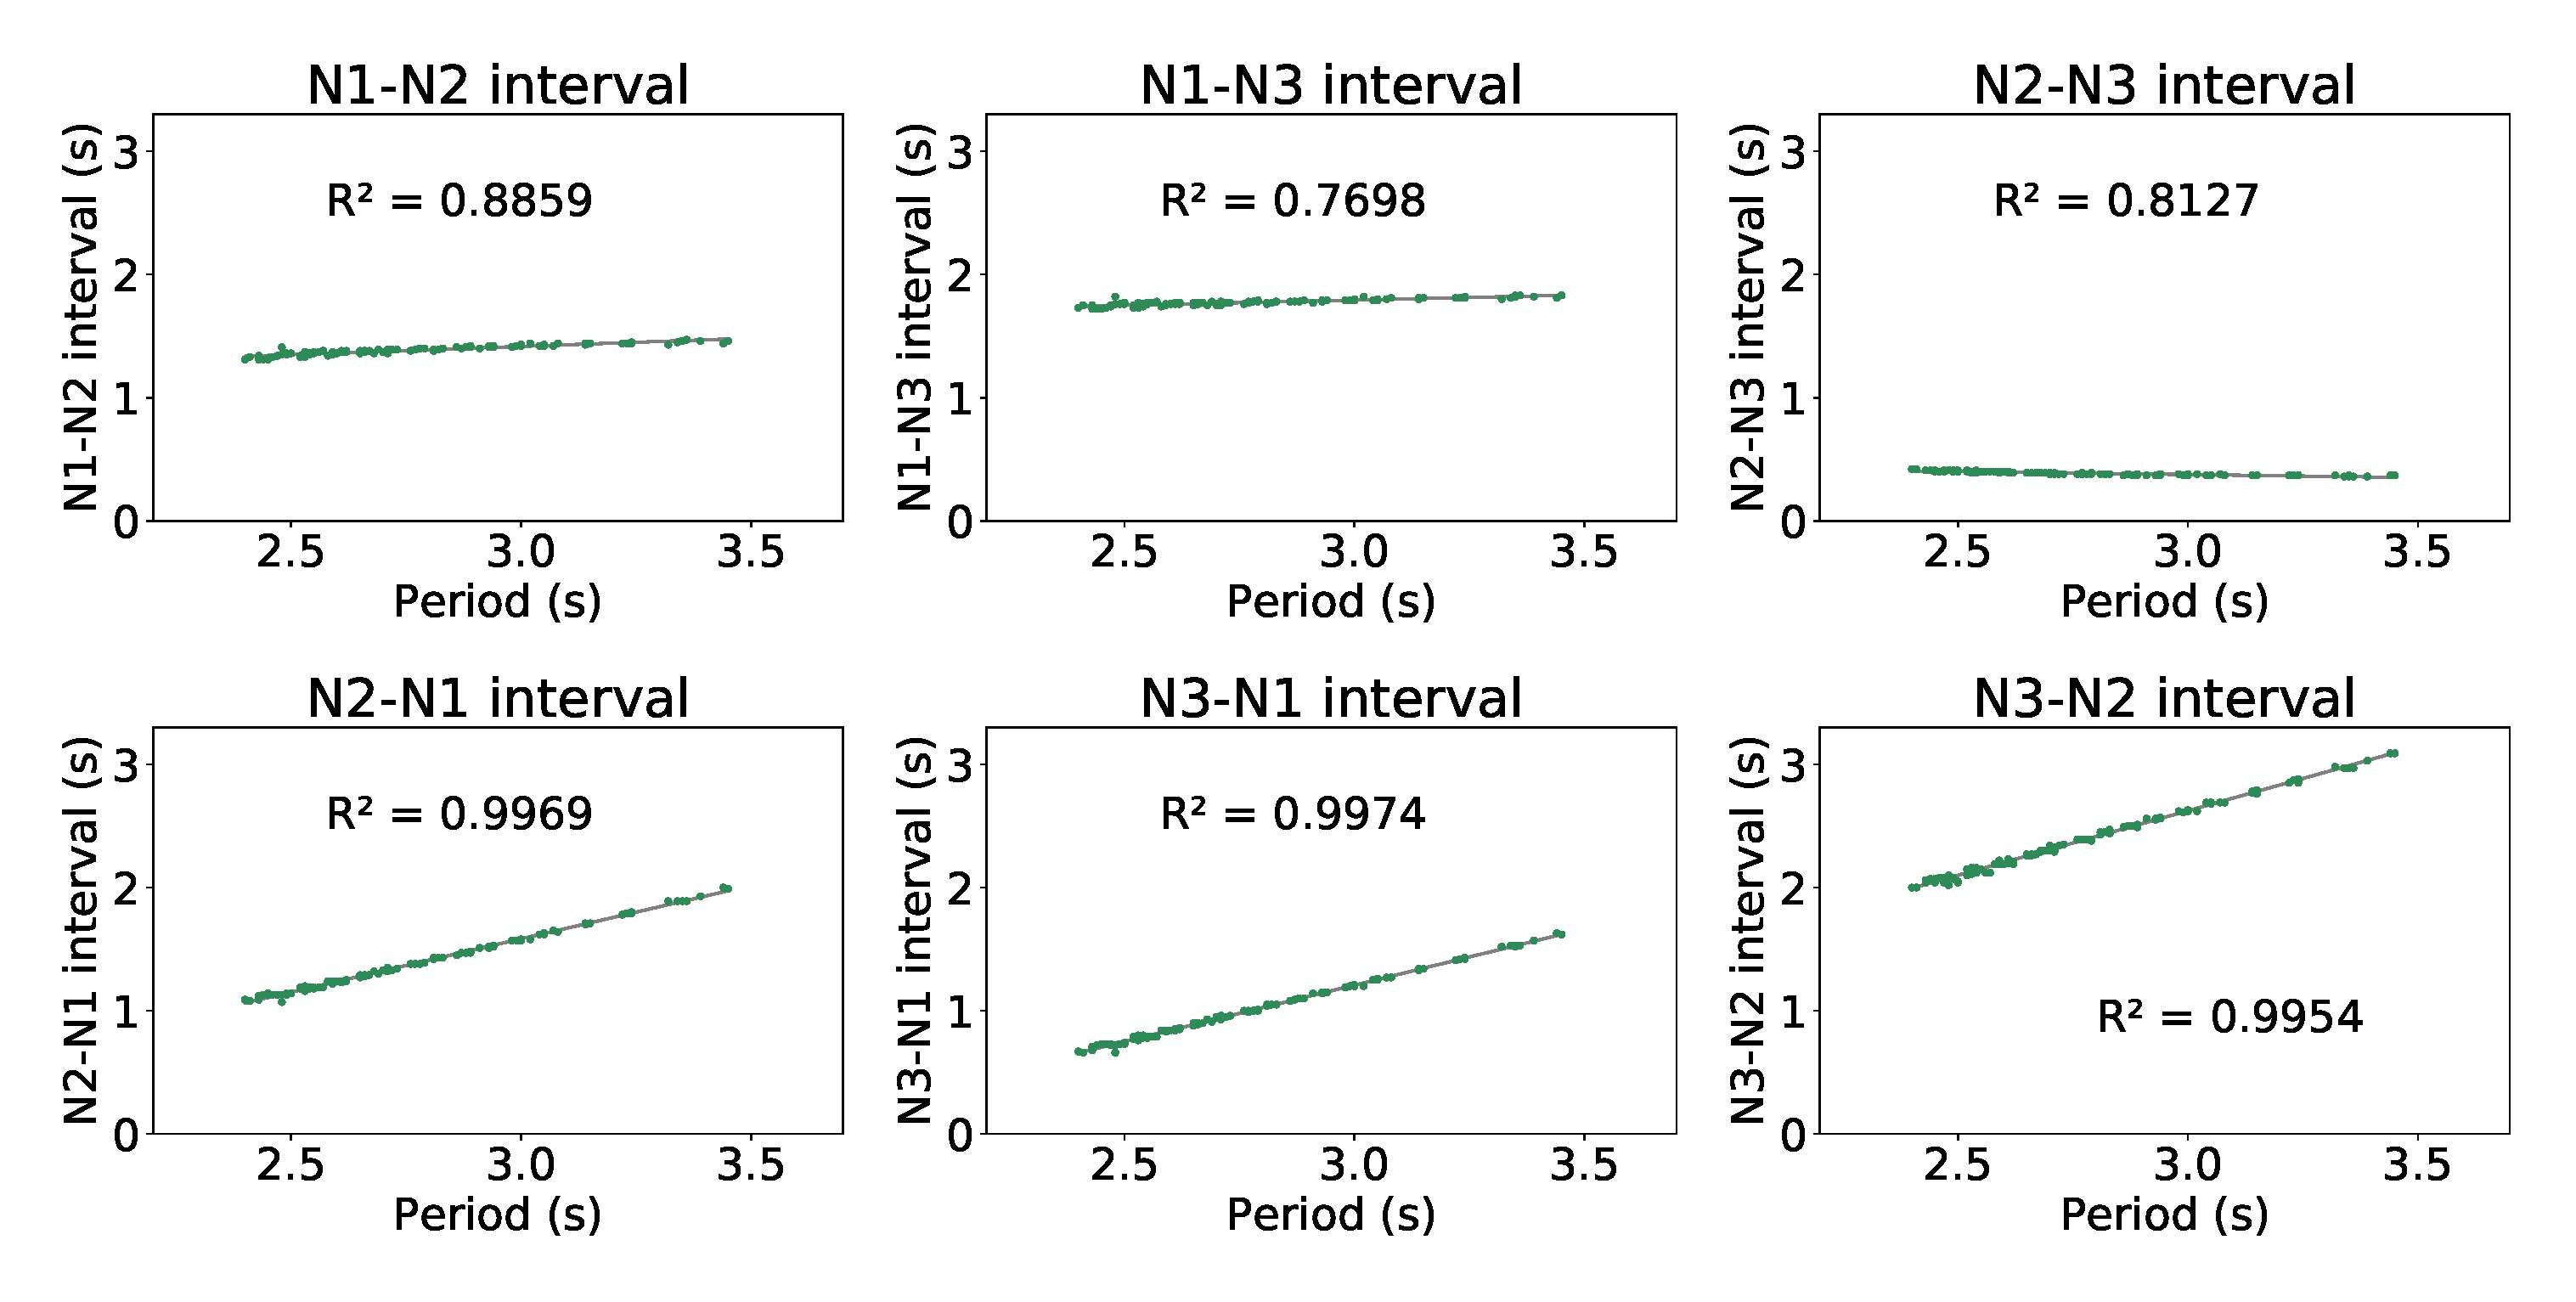
\includegraphics[width=\textwidth]{img/results-paper-modelo/figure8_row2-3.eps}
%      
%  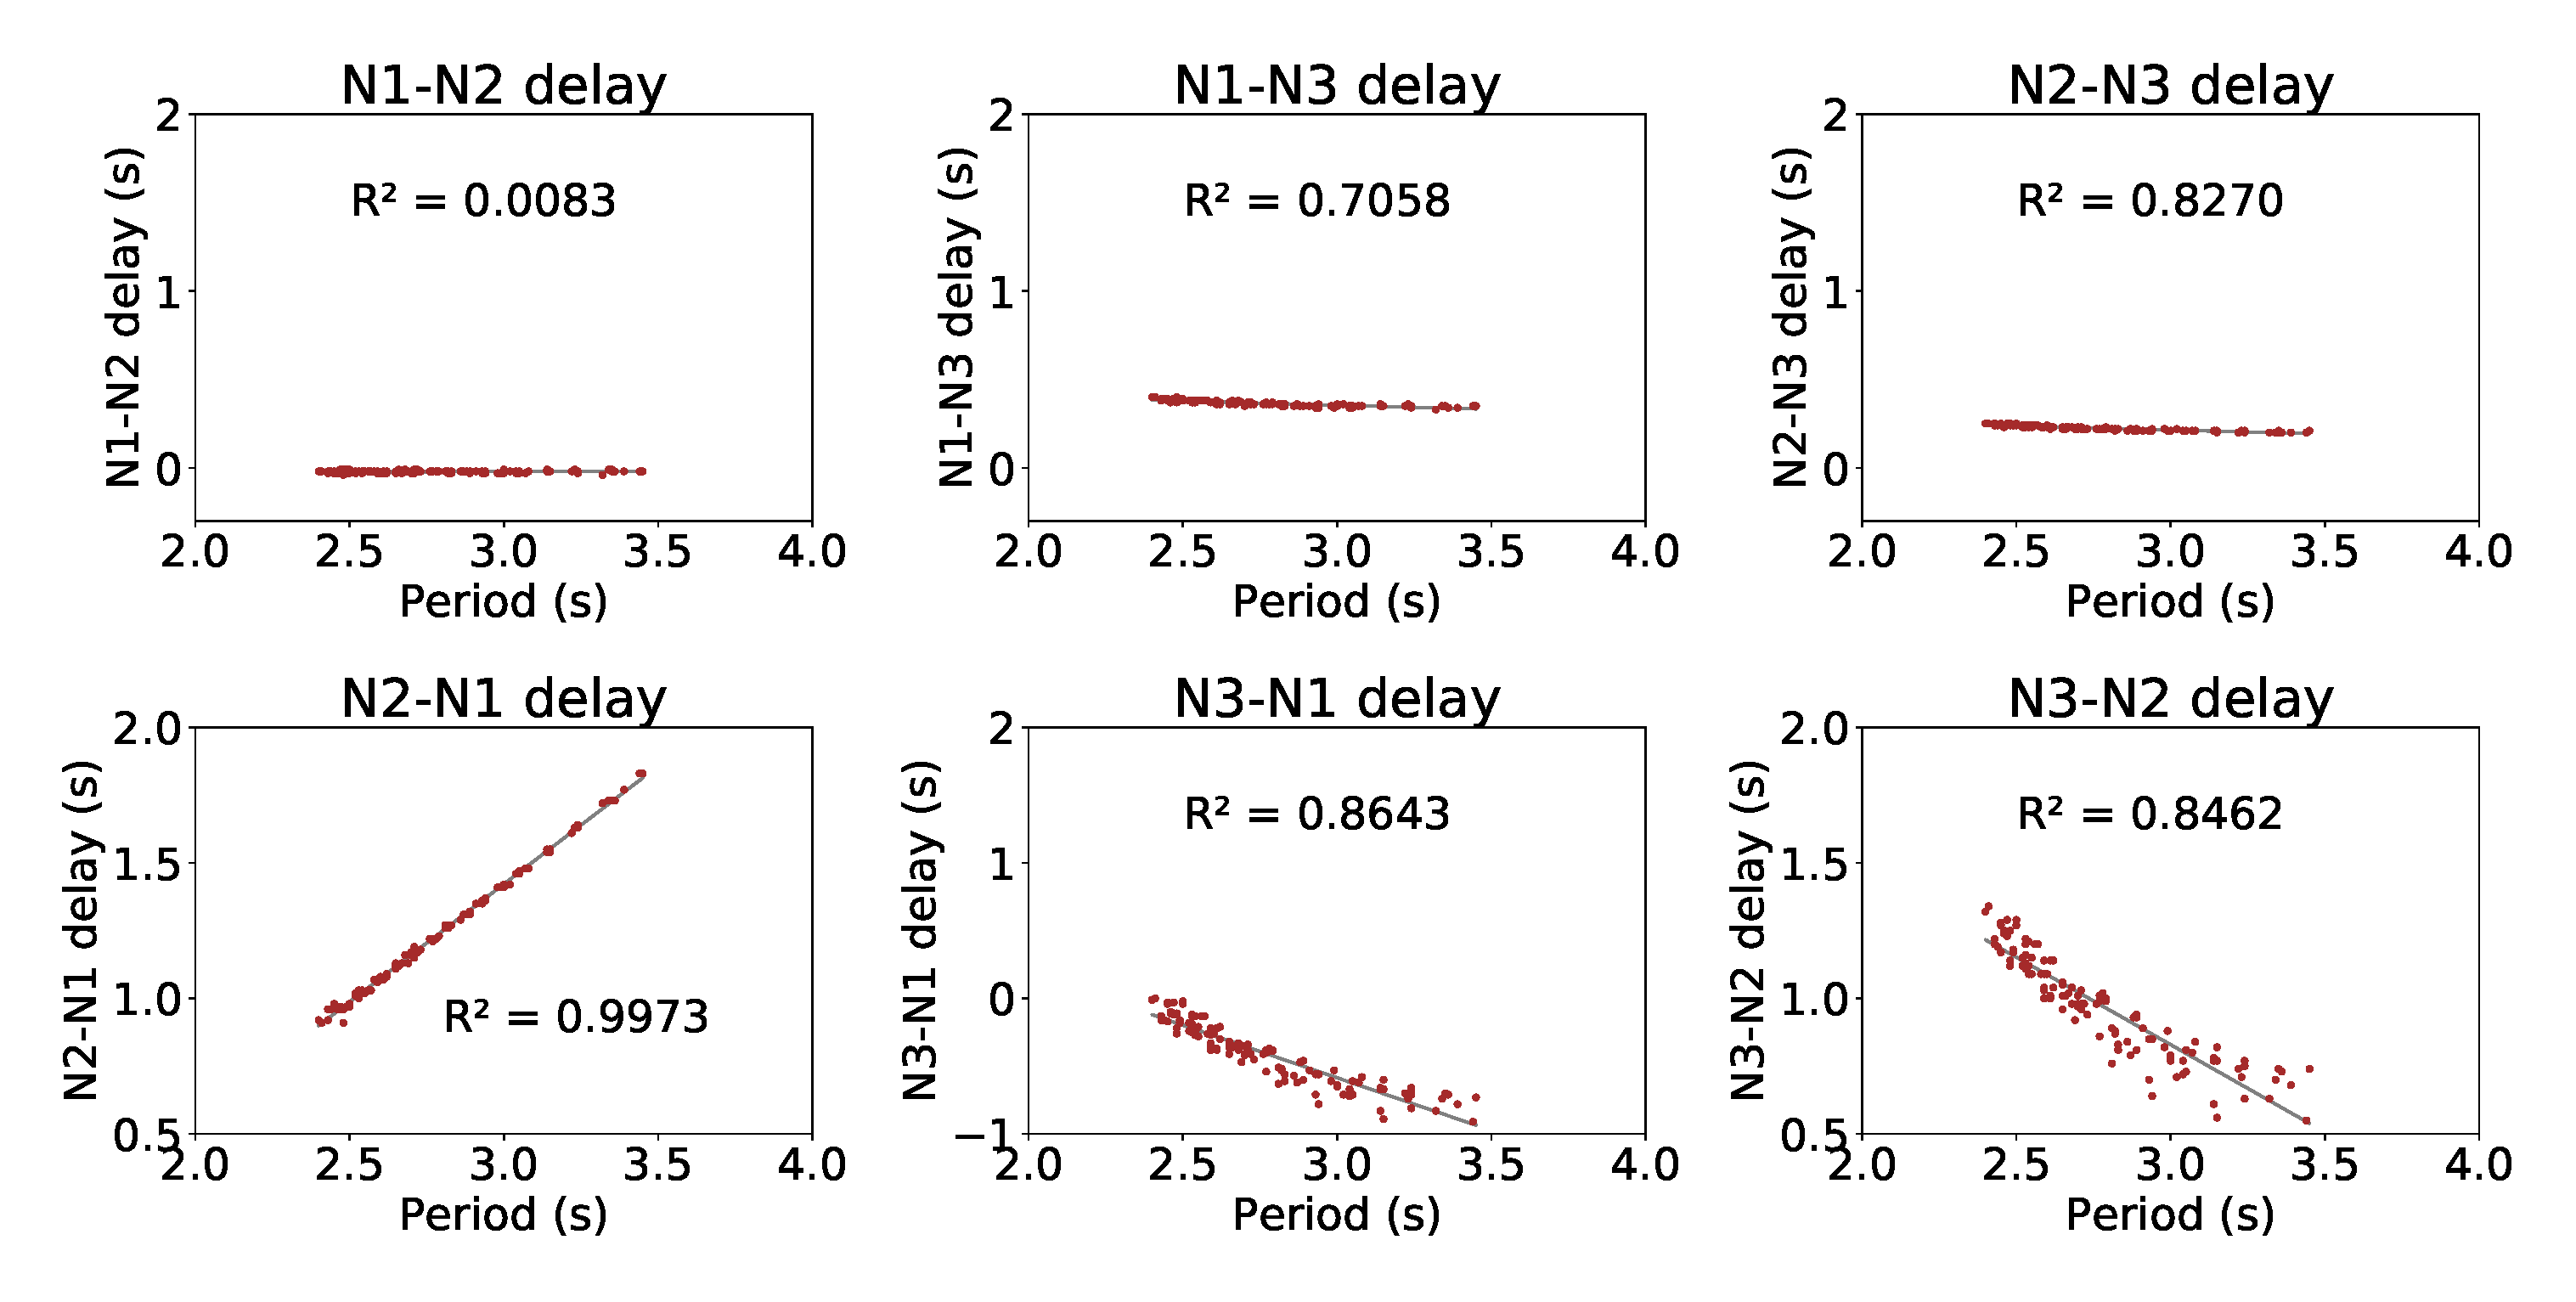
\includegraphics[width=\textwidth]{img/results-paper-modelo/figure8_row4-5.eps}
%
%    \caption{Interval correlations to Period for N3t-driven simulation. First row: Burst duration. Second and third row: Two-neuron intervals. Forth and fifth row: Two-neuron delays.}
%    \label{fig:invariant n3t test17}
%\end{figure}
%
%


%\begin{figure}[hbt!]
%	\begin{minipage}[b]{0.45\textwidth}
%		\centering
%		\includegraphics[width=\textwidth]{invariants/data/MODEL/n3t_driven/images/3phases/_boxplot.pdf}
%	\end{minipage}
%	\begin{minipage}[b]{0.53\textwidth}
%		\centering
%		\begin{minipage}[b]{\textwidth}
%			\centering
%			\includegraphics[width=\textwidth]{invariants/data/MODEL/n3t_driven/images/3phases/_durations.pdf}
%		\end{minipage}\
%		\begin{minipage}[b]{\textwidth}
%			\centering
%			\includegraphics[width=\textwidth]{invariants/data/MODEL/n3t_driven/images/3phases/_intervals.pdf}
%		\end{minipage}\
%		\begin{minipage}[b]{\textwidth}
%			\centering
%			\includegraphics[width=\textwidth]{invariants/data/MODEL/n3t_driven/images/3phases/_delays.pdf}
%		\end{minipage}
%	\end{minipage}
%	\caption{a) Box-plots of the sequence intervals under N3t neuron stimulation. b) Interval correlations to Period for N3t-driven simulation. First row: Burst duration. Second and third row: Two-neuron intervals. Forth and fifth row: Two-neuron delays}
%	\label{fig:invariant n3t test17}
%\end{figure}
%




\subsection{SO driven variability}

The same protocol was implemented with a ramp stimulation applied to SO to induce variability, using the injected current values shown in Table \ref{table:inj values} for each neuron. Events were detected and all intervals were measured (Fig. \ref{fig:intervals}) and their variability was characterized. %This neuron has also been used in previous studies with stimulation protocols both in electrophysiological experiments and in model simulations due to its important role in rhythm activation and modulation. ***se podría quitar, si no hay que poner las referencias otra vez****

Figure \ref{fig:invariant so boxplot} displays the box-plot representing the distinct interval variability. In this case, we found more intervals showing large variability than in the previous cases. N2v intervals, as it happened in the previous results, show low variability. %, which indicates that period variability is more likely a consequence of N3t and N1M activity.
N1M and N3t neurons show high variability in their burst duration intervals, being N1M even more variable than N3t, as opposed to the previous results when the stimulation was introduced in other cells. All intervals derived from these two neurons have high variability and a similar structure. %Therefore, now the intervals which show low variability are the ones related to N2v. 

% In spite all this, what remains constant from N1M-driven simulation is the variability of the N3-N2 interval, which includes both N1M and N3t burst duration, being N3-N2 the most variable one, and the closest to the period variability.%distribution

% Since in this case there are more neurons showing high variability, we should expect finding more correlations when plotting each interval against the period.  ***también deberíamos quitar redundancia aquí***
% Hence, as it happened in the previous results, all intervals related to N3t show dynamical invariants, but this time they are also present in the ones related with N1M, which show a high variability. 
% the intervals with more variability and, thus, those that had a more similar variability structure to the period, were the ones that showed dynamical invariants%(a highest linear relation to the period)


Figure \ref{fig:invariant so test19} displays the corresponding correlation analysis between all intervals and the period. %In this case, as it happens in the box-plot, there are found different results
In this case, we found correlations in the same intervals as before: N2-N1, N3-N1, N3-N2 intervals and N2-N1 delay; which are the intervals related to N3t burst duration. However, under SO stimulation,  N1-N2, N1-N3 intervals were also highly correlated to the period. Even the correlation for N3-N2 delay considerably increased in relation to the other stimulation conditions. These intervals are the ones related to N1M neuron activity, and were also the most variable ones.  These results reproduce the experimentally analyzed effects set out in \parencite{elliott_temporal_1991}, when rhythm and variability was induced by injecting current into a living SO neuron.

%Furthermore, it is important to notice that N3-N1 delay is negative again ****por qué es importante si es lo mismo que antes****. As it happened in N3t-driven simulation, this means there is a constant overlapping between N3 and N1 in each cycle, i.e. N3t burst interval is coming earlier. This can be also appreciated in boxplot, since this interval is represented below 0. 

Compared to the N1M and N3t stimulation results, there is another difference when driving the rhythm with SO: burst duration is much shorter, so the period and the rest of intervals are consequently smaller. Therefore, when driving the rhythm by SO, the period variability seems to arise from both N3t as well as by N1M. 
%the model produces a rhythm where the information about period duration seems to be carried by N3t as well as by N1M. 
%
%\begin{figure}[h!]
%    \centering
%\includegraphics[width=\textwidth]{img/results-paper-modelo/figure9.eps}
%\caption{Box-plots of the sequence intervals under SO neuron stimulation.}
%\label{fig:invariant so boxplot}
%\end{figure}
%\clearpage
%\newpage
%\begin{figure}[h!]
%    \centering
%\includegraphics[width=\textwidth]{img/results-paper-modelo/figure10_row1.eps}
%  \includegraphics[width=\textwidth]{img/results-paper-modelo/figure10_row2-3.eps}
%      
%  \includegraphics[width=\textwidth]{img/results-paper-modelo/figure10_row4-5.eps}%
%
%    \caption{Interval correlations to Period for SO-driven simulation. First row: Burst duration. Second and third row: Two-neuron intervals. Forth and fifth row: Two-neuron delays.}
%    \label{fig:invariant so test19}
%\end{figure}
%

%\begin{figure}[hbt!]
%	\begin{minipage}[b]{0.45\textwidth}
%		\centering
%		\includegraphics[width=\textwidth]{invariants/data/MODEL/so_driven/images/3phases/_boxplot.pdf}
%	\end{minipage}
%	\begin{minipage}[b]{0.53\textwidth}
%		\centering
%		\begin{minipage}[b]{\textwidth}
%			\centering
%			\includegraphics[width=\textwidth]{invariants/data/MODEL/so_driven/images/3phases/_durations.pdf}
%		\end{minipage}\
%		\begin{minipage}[b]{\textwidth}
%			\centering
%			\includegraphics[width=\textwidth]{invariants/data/MODEL/so_driven/images/3phases/_intervals.pdf}
%		\end{minipage}\
%		\begin{minipage}[b]{\textwidth}
%			\centering
%			\includegraphics[width=\textwidth]{invariants/data/MODEL/so_driven/images/3phases/_delays.pdf}
%		\end{minipage}
%	\end{minipage}
%	\caption{a) Box-plots of the sequence intervals under SO neuron stimulation. b) Interval correlations to Period for SO-driven simulation. First row: Burst duration. Second and third row: Two-neuron intervals. Forth and fifth row: Two-neuron delays.}
%	\label{fig:invariant so test19}
%\end{figure}



\subsection{Time intervals relations cycle-by-cycle beyond period}
We saw so far the sequential dynamical invariants in terms of strong linear relationships between the distinct intervals in a cycle and the period, however, studying the relations between all intervals can also show interesting information about the temporal variability distribution in the ongoing activity \cite{}. In Figs \ref{fig;model n1m stimulation pairplot} to \ref{fig:model so stimulation pairplot} there is a representation of all possible combinations of the defined intervals. 



\begin{figure}[htbp]
	\centering
	\includegraphics[width=\textwidth]{./invariants/data/MODEL/n1m_driven/images/3phases/_output_pairplot.png}
	\caption{\textbf{N1M stimulation}: Panel of intervals distribution and dynamical invariants for the two phases in the CPG for activity when N1M is stimulated.}
	\label{fig:model n1m stimulation pairplot}
\end{figure}
 

\begin{figure}[htbp]
	\centering
	\includegraphics[width=\textwidth]{./invariants/data/MODEL/n3t_driven/images/3phases/_output_pairplot.png}
	\caption{\textbf{N3t stimulation}: Panel of intervals distribution and dynamical invariants for the two phases in the CPG for activity when N3t is stimulated.}
	\label{fig:model n3t stimulation pairplot}
\end{figure}


\begin{figure}[htbp]
	\centering
	\includegraphics[width=\textwidth]{./invariants/data/MODEL/so_driven/images/3phases/_output_pairplot.png}
	\caption{\textbf{SO stimulation}: Panel of intervals distribution and dynamical invariants for the two phases in the CPG for activity when SO is stimulated.}
	\label{fig:model so stimulation pairplot}
\end{figure}


\subsection{Comparison with 2 phases intervals}
Although during this section we analyzed the sequential dynamical invariants in for 3 phases, we can also define the intervals for two phases of the neurons, taking as reference for example, N1 and N3. This is the case in the work by \cite{elices_robust_2019}, and in the following section we will also use two phases for some of the recordings were the N2 phase was not possible to define. Therefore, in this subsection we will show an example of the intervals conformed with two phase, to compare and analyze the differences in the dynamical invariants. 


\begin{figure}[htbp]
	\centering
	\includegraphics[width=\textwidth]{./invariants/data/MODEL/n1m_driven/images/2phases/_output_pairplot.png}
	\caption{\textbf{N1M stimulation}: Panel of intervals distribution and dynamical invariants for the two phases in the CPG for activity when N1M is stimulated.}
	\label{fig:model n1m stimulation pairplot 2phases}
\end{figure}



\begin{figure}[hbt!]
	\begin{minipage}[b]{0.53\textwidth}
		\centering
		\begin{minipage}[b]{\textwidth}
			\centering
			\includegraphics[width=\textwidth]{invariants/data/MODEL/n1m_driven/images/3phases/_durations.pdf}
		\end{minipage}\
		\begin{minipage}[b]{\textwidth}
			\centering
			\includegraphics[width=\textwidth]{invariants/data/MODEL/n1m_driven/images/3phases/_intervals.pdf}
		\end{minipage}\
		\begin{minipage}[b]{\textwidth}
			\centering
			\includegraphics[width=\textwidth]{invariants/data/MODEL/n1m_driven/images/3phases/_delays.pdf}
		\end{minipage}
	\end{minipage}
	\begin{minipage}[b]{0.45\textwidth}
		\centering
		\begin{minipage}[b]{\textwidth}
			\centering
			\includegraphics[width=\textwidth]{invariants/data/MODEL/n1m_driven/images/2phases/_durations.pdf}
		\end{minipage}\
		\begin{minipage}[b]{\textwidth}
			\centering
			\includegraphics[width=\textwidth]{invariants/data/MODEL/n1m_driven/images/2phases/_intervals.pdf}
		\end{minipage}\
		\begin{minipage}[b]{\textwidth}
			\centering
			\includegraphics[width=\textwidth]{invariants/data/MODEL/n1m_driven/images/2phases/_delays.pdf}
		\end{minipage}
	
		\vspace{50pt}
	\end{minipage}
	\caption{a).Box-plots of the  sequence intervals under N1M neuron stimulation. b) Interval correlations to period for N1M-driven simulation. First row: Burst duration. Second and third row: Two-neuron intervals. Forth and fifth row: Two-neuron delays. Linear relationships are quantified by the $R^2$ values of the regression.}
	\label{fig:invariant n1m}
\end{figure}




%
%
%\begin{figure}[htbp]
%	\centering
%	\includegraphics[width=\textwidth]{./invariants/data/MODEL/n3t_driven/images/2phases/_output_pairplot.png}
%	\caption{\textbf{N3t stimulation}: Panel of intervals distribution and dynamical invariants for the two phases in the CPG for activity when N3t is stimulated.}
%	\label{fig:model n3t stimulation pairplot 2phases}
%\end{figure}
%
%
%\begin{figure}[htbp]
%	\centering
%	\includegraphics[width=\textwidth]{./invariants/data/MODEL/so_driven/images/2phases/_output_pairplot.png}
%	\caption{\textbf{SO stimulation}: Panel of intervals distribution and dynamical invariants for the two phases in the CPG for activity when SO is stimulated.}
%	\label{fig:model so stimulation pairplot 2phases}
%\end{figure}

\section{Characterization of variability in bursting models}
\label{c-invariants-model}
\section{Experimental results in \textit{Lymnaea Stagnalis}}
When studying temporal structures in neural dynamics, the definition of the time references is a key first point. In the computational analysis in the previous section, the time reference to define the intervals where first and last spike in the burts. In that case, as well as in the case of inter-neurons in \textit{C. maenas} the CPG phases are directly related with the bursting activity of these neurons. However, in the case of \textit{Lymnaea stagnalis}, activity is usually characterized using recordings from both inter-neurons and moto-neurons \parencite{elliot, benjamin, crossley}. This leads to a more flexible reference of the time references, so for this analysis, references will be defined by the phase and each phase will be bounded by different neurons. For example, in Figure \ref{fig:example lymnaea phases recording} the three phases in the  CPG are marked over the recording, note how it can be delimited by the neurons in the circuit but some of the moto-neurons cover several phases and that phases are delimited not only by the spikes but the hyperpolarization periods. Therefore, to characterize the time sequences in the feeding CPG, we need compound reference from several neural recordings that can be summarized as in Table \ref{table:cpg ref intervals}

%\TODO revisar
Table \ref{table:tabla spikes} displays a summary of some neurons involved in each phase. \todo{viene del tfm revisar}

% Please add the following required packages to your document preamble:
% \usepackage{multirow}
\begin{table}[htb!]
	\begin{tabular}{cl|l|ll}
		\multicolumn{1}{l}{}                                 & \multicolumn{1}{c|}{\textbf{N1}} & \multicolumn{1}{c|}{\textbf{N2}} & \multicolumn{1}{c}{\textbf{N3}} &  \\
		\multicolumn{1}{c|}{\multirow{2}{*}{\textbf{Start}}} & Last spike of N3t/B3             & Inhibition of B5                 & First spike of B8               &  \\
		\multicolumn{1}{c|}{}                                & Depolarization in B1             &                                  &                                 &  \\ \cline{1-4}
		\multicolumn{1}{c|}{\multirow{2}{*}{\textbf{End}}}   & Last spike of B5                 & First spike of B8                & Last spike of N3t/B3            &  \\
		\multicolumn{1}{c|}{}                                & Hyperpolarization in B1          &                                  &                                 & 
	\end{tabular}
	\caption{Time reference boundaries for the three phases in the feeding CPG}
	\label{table:cpg ref intervals}
\end{table}


\begin{table}[h!]
	\centering
	\begin{tabular}{lccc}
		Neuron                                           & \multicolumn{1}{l}{Protraction} & \multicolumn{1}{l}{Rasp} & \multicolumn{1}{l}{Swallow} \\ \hline
		Interneuron                                     & N1                              & N2                       & N3                          \\
		& \multicolumn{1}{l}{}            & \multicolumn{1}{l}{}     & \multicolumn{1}{l}{}        \\
		\multicolumn{1}{c}{\multirow{3}{*}{Motoneuron}} & B7                              & B10                      & B3                        \\
		\multicolumn{1}{c}{}                            & B6                              & B4                       & B9                        \\
		\multicolumn{1}{c}{}                            & B1                              &                          &                         
	\end{tabular}
	\caption{Neuron participation in feeding phases.}
	\label{table:tabla spikes}
\end{table}



\begin{figure}[bth!]
\centering
\includegraphics[width=\textwidth]{img/invariants/example_phases_1.pdf}
\\
\vspace{10pt}
\includegraphics[width=\textwidth]{img/invariants/example_phases_2.pdf}
\caption{Delimitation of phases in the feeding CPG of \textit{Lymnaea stagnalis} based on different recordings.}
\label{fig:example lymnaea phases recording}
\end{figure}



\subsubsection{Invariants in spontaneous activity}

\begin{figure}[htbp]
	\centering
	\begin{minipage}[b]{\textwidth}
		\centering
		\includegraphics[width=\textwidth]{./invariants/data/SUSSEX/prep1/images/spontaneous_2phases_time_cycle.pdf}
		\includegraphics[width=\textwidth,height=0.2\textheight]{./invariants/data/SUSSEX/prep1/images/spontaneous_2phases_boxplot_h.pdf}		
	\end{minipage}
	\centering
	\begin{minipage}{\textwidth}
%		\begin{minipage}[b]{0.53\textwidth}
%			\centering
%			\begin{minipage}[b]{\textwidth}
%				\centering
%				\includegraphics[width=\textwidth]{./invariants/data/SUSSEX/prep1/images/spontaneous_durations.pdf}
%			\end{minipage}\\
%			\begin{minipage}[b]{\textwidth}
%				\centering
%				\includegraphics[width=\textwidth]{./invariants/data/SUSSEX/prep1/images/spontaneous_intervals.pdf}
%			\end{minipage}\\
%			\begin{minipage}[b]{\textwidth}
%				\centering
%				\includegraphics[width=\textwidth]{./invariants/data/SUSSEX/prep1/images/spontaneous_delays.pdf}
%			\end{minipage}
%		\end{minipage}
		\includegraphics[width=\textwidth]{./invariants/data/SUSSEX/prep1/images/spontaneous_2phases_pairplot_oneside_cycle.png}
%		\includegraphics[width=\textwidth]{./invariants/data/SUSSEX/prep1/images/spontaneous_2phases_pairplot_oneside.png}
%		\includegraphics{./invariants/data/SUSSEX/prep1/images/spontaneous_2phases_pairplot_oneside.png}
	\end{minipage}
	\caption{\textbf{Spontaneous case1}: Panel of intervals distribution and dynamical invariants for the three phases in the CPG for spontaneous activity.}
	\label{fig:prep1 reduced panel}
\end{figure}


\begin{figure}[htbp]
	\centering
	\begin{minipage}[b]{\textwidth}
		\centering
		\includegraphics[width=\textwidth,height=0.1\textheight]{./invariants/data/SUSSEX/prep1/images/spontaneous_signal_intervals_zoom.pdf}
		\includegraphics[width=\textwidth]{./invariants/data/SUSSEX/prep1/images/spontaneous_signal_intervals_cycle.pdf}
		\includegraphics[width=\textwidth]{./invariants/data/SUSSEX/prep1/images/spontaneous_time_cycle.pdf}
	\end{minipage}
	\centering
	\begin{minipage}{0.9\textwidth}
		\begin{minipage}[b]{0.45\textwidth}
			\centering
			\includegraphics[width=\textwidth]{./invariants/data/SUSSEX/prep1/images/spontaneous_boxplot.pdf}
		\end{minipage}
		%	\hfill
		\begin{minipage}[b]{0.53\textwidth}
			\centering
			\begin{minipage}[b]{\textwidth}
				\centering
				\includegraphics[width=\textwidth]{./invariants/data/SUSSEX/prep1/images/spontaneous_durations.pdf}
			\end{minipage}\\
			\begin{minipage}[b]{\textwidth}
				\centering
				\includegraphics[width=\textwidth]{./invariants/data/SUSSEX/prep1/images/spontaneous_intervals.pdf}
			\end{minipage}\\
			\begin{minipage}[b]{\textwidth}
				\centering
				\includegraphics[width=\textwidth]{./invariants/data/SUSSEX/prep1/images/spontaneous_delays.pdf}
			\end{minipage}
		\end{minipage}
	\end{minipage}
	\caption{\textbf{Spontaneous case1}: Panel of intervals distribution and dynamical invariants for the three phases in the CPG for spontaneous activity.}
	\label{fig:prep1 invariants}
\end{figure}

\begin{figure}[htbp]
	\centering
	\begin{minipage}[b]{\textwidth}
		\centering
		\includegraphics[width=\textwidth,height=0.1\textheight]{./invariants/data/SUSSEX/prep1/images/spontaneous_2phases_signal_intervals_zoom.pdf}
		\includegraphics[width=\textwidth]{./invariants/data/SUSSEX/prep1/images/spontaneous_2phases_signal_intervals_cycle.pdf}
		\includegraphics[width=\textwidth]{./invariants/data/SUSSEX/prep1/images/spontaneous_2phases_time_cycle.pdf}
	\end{minipage}
	\centering
	\begin{minipage}{0.9\textwidth}
		\begin{minipage}[b]{0.45\textwidth}
			\centering
			\includegraphics[width=\textwidth]{./invariants/data/SUSSEX/prep1/images/spontaneous_2phases_boxplot.pdf}
		\end{minipage}
		%	\hfill
		\begin{minipage}[b]{0.53\textwidth}
			\centering
			\begin{minipage}[b]{\textwidth}
				\centering
				\includegraphics[width=\textwidth]{./invariants/data/SUSSEX/prep1/images/spontaneous_2phases_durations.pdf}
			\end{minipage}\\
			\begin{minipage}[b]{\textwidth}
				\centering
				\includegraphics[width=\textwidth]{./invariants/data/SUSSEX/prep1/images/spontaneous_2phases_intervals.pdf}
			\end{minipage}\\
			\begin{minipage}[b]{\textwidth}
				\centering
				\includegraphics[width=\textwidth]{./invariants/data/SUSSEX/prep1/images/spontaneous_2phases_delays.pdf}
			\end{minipage}
		\end{minipage}
	\end{minipage}
	\caption{\textbf{Spontaneous case1}: Panel of intervals distribution and dynamical invariants for two phases in the CPG for spontaneous activity.}
	\label{fig:prep1 2 phases invariants}
\end{figure}
%
%\begin{figure}[bth!]
%	\centering
%	\includegraphics[width=\textwidth]{img/invariants/prep1_3 intervals panel.pdf}
%	\caption{Boxplots and correlation of main intervals in spontaneous activity of \textit{L. stagnalis}}
%	\label{fig:prep1 invariants}
%\end{figure}



%\begin{figure}[bth!]
%	\centering
%	\includegraphics[width=0.5\textwidth]{img/invariants/prep3_3 intervals panel.pdf}
%	\caption{Boxplots and correlation of main intervals in spontaneous activity of \textit{L. stagnalis}}
%	\label{fig:prep3 invariants}
%\end{figure}



\begin{figure}[htbp]
	\centering
	\begin{minipage}[b]{\textwidth}
		\centering
		\includegraphics[width=\textwidth,height=0.1\textheight]{./invariants/data/SUSSEX/prep2/images/spontaneous_signal_intervals_zoom.pdf}
		\includegraphics[width=\textwidth]{./invariants/data/SUSSEX/prep2/images/spontaneous_signal_intervals_cycle.pdf}
		\includegraphics[width=\textwidth]{./invariants/data/SUSSEX/prep2/images/spontaneous_time_cycle.pdf}
	\end{minipage}
	\begin{minipage}{0.9\textwidth}
		\centering
		\begin{minipage}[b]{0.45\textwidth}
			\centering
			\includegraphics[width=\textwidth]{./invariants/data/SUSSEX/prep2/images/spontaneous_boxplot.pdf}
		\end{minipage}
		%	\hfill
		\begin{minipage}[b]{0.53\textwidth}
			\centering
			\begin{minipage}[b]{\textwidth}
				\centering
				\includegraphics[width=\textwidth]{./invariants/data/SUSSEX/prep2/images/spontaneous_durations.pdf}
			\end{minipage}\\
			\begin{minipage}[b]{\textwidth}
				\centering
				\includegraphics[width=\textwidth]{./invariants/data/SUSSEX/prep2/images/spontaneous_intervals.pdf}
			\end{minipage}\\
			\begin{minipage}[b]{\textwidth}
				\centering
				\includegraphics[width=\textwidth]{./invariants/data/SUSSEX/prep2/images/spontaneous_delays.pdf}
			\end{minipage}
		\end{minipage}
	\end{minipage}
	\caption{\textbf{Spontaneous case2}: Panel of intervals distribution and dynamical invariants for the three phases in the CPG for spontaneous activity.}
	\label{fig:prep2 invariants}
\end{figure}


\begin{figure}[htbp]
	\centering
	\begin{minipage}[b]{\textwidth}
		\centering
		\includegraphics[width=\textwidth,height=0.1\textheight]{./invariants/data/SUSSEX/prep2/images/spontaneous_2phases_signal_intervals_zoom.pdf}
		\includegraphics[width=\textwidth]{./invariants/data/SUSSEX/prep2/images/spontaneous_2phases_signal_intervals_cycle.pdf}
		\includegraphics[width=\textwidth]{./invariants/data/SUSSEX/prep2/images/spontaneous_2phases_time_cycle.pdf}
	\end{minipage}
	\begin{minipage}{0.9\textwidth}
		\centering
		\begin{minipage}[b]{0.45\textwidth}
			\centering
			\includegraphics[width=\textwidth]{./invariants/data/SUSSEX/prep2/images/spontaneous_2phases_boxplot.pdf}
		\end{minipage}
		%	\hfill
		\begin{minipage}[b]{0.53\textwidth}
			\centering
			\begin{minipage}[b]{\textwidth}
				\centering
				\includegraphics[width=\textwidth]{./invariants/data/SUSSEX/prep2/images/spontaneous_2phases_durations.pdf}
			\end{minipage}\\
			\begin{minipage}[b]{\textwidth}
				\centering
				\includegraphics[width=\textwidth]{./invariants/data/SUSSEX/prep2/images/spontaneous_2phases_intervals.pdf}
			\end{minipage}\\
			\begin{minipage}[b]{\textwidth}
				\centering
				\includegraphics[width=\textwidth]{./invariants/data/SUSSEX/prep2/images/spontaneous_2phases_delays.pdf}
			\end{minipage}
		\end{minipage}
	\end{minipage}
	\caption{\textbf{Spontaneous case2}: Panel of intervals distribution and dynamical invariants for two phases in the CPG for spontaneous activity.}
	\label{fig:prep2 2phase invariants}
\end{figure}

\begin{figure}[htbp]
	\centering
	\begin{minipage}[b]{\textwidth}
		\centering
		\includegraphics[width=\textwidth,height=0.1\textheight]{./invariants/data/SUSSEX/prep3/images/prep3_3phases_signal_intervals_zoom.pdf}
		\includegraphics[width=\textwidth]{./invariants/data/SUSSEX/prep3/images/prep3_signal_intervals_cycle.pdf}
		\includegraphics[width=\textwidth]{./invariants/data/SUSSEX/prep3/images/prep3_time_cycle.pdf}
	\end{minipage}
	\begin{minipage}{0.9\textwidth}
		\centering
		\begin{minipage}[b]{0.45\textwidth}
			\centering
			\includegraphics[width=\textwidth]{./invariants/data/SUSSEX/prep3/images/prep3_boxplot.pdf}
		\end{minipage}
		%	\hfill
		\begin{minipage}[b]{0.53\textwidth}
			\centering
			\begin{minipage}[b]{\textwidth}
				\centering
				\includegraphics[width=\textwidth]{./invariants/data/SUSSEX/prep3/images/prep3_durations.pdf}
			\end{minipage}\\
			\begin{minipage}[b]{\textwidth}
				\centering
				\includegraphics[width=\textwidth]{./invariants/data/SUSSEX/prep3/images/prep3_intervals.pdf}
			\end{minipage}\\
			\begin{minipage}[b]{\textwidth}
				\centering
				\includegraphics[width=\textwidth]{./invariants/data/SUSSEX/prep3/images/prep3_delays.pdf}
			\end{minipage}
		\end{minipage}
	\end{minipage}
	\caption{\textbf{Spontaneous case3}: Panel of intervals distribution and dynamical invariants for two phases in the CPG for spontaneous activity.}
	\label{fig:prep3 2phases invariants}
\end{figure}

\begin{figure}[htbp]
	\centering
	\begin{minipage}[b]{\textwidth}
		\centering
		\includegraphics[width=\textwidth,height=0.1\textheight]{./invariants/data/SUSSEX/prep3/images/prep3_3phases_signal_intervals_zoom.pdf}
		\includegraphics[width=\textwidth]{./invariants/data/SUSSEX/prep3/images/prep3_3phases_signal_intervals_cycle.pdf}
		\includegraphics[width=\textwidth]{./invariants/data/SUSSEX/prep3/images/prep3_3phases_time_cycle.pdf}
	\end{minipage}
	\centering
	\begin{minipage}{0.9\textwidth}
		\begin{minipage}[b]{0.45\textwidth}
			\centering
			\includegraphics[width=\textwidth]{./invariants/data/SUSSEX/prep3/images/prep3_3phases_boxplot.pdf}
		\end{minipage}
		%	\hfill
		\begin{minipage}[b]{0.53\textwidth}
			\centering
			\begin{minipage}[b]{\textwidth}
				\centering
				\includegraphics[width=\textwidth]{./invariants/data/SUSSEX/prep3/images/prep3_3phases_durations.pdf}
			\end{minipage}\\
			\begin{minipage}[b]{\textwidth}
				\centering
				\includegraphics[width=\textwidth]{./invariants/data/SUSSEX/prep3/images/prep3_3phases_intervals.pdf}
			\end{minipage}\\
			\begin{minipage}[b]{\textwidth}
				\centering
				\includegraphics[width=\textwidth]{./invariants/data/SUSSEX/prep3/images/prep3_3phases_delays.pdf}
			\end{minipage}
		\end{minipage}
	\end{minipage}
	\caption{\textbf{Spontaneous case3}: Panel of intervals distribution and dynamical invariants for the three phases in the CPG for spontaneous activity.}
	\label{fig:prep3 invariants}
\end{figure}



\subsubsection{Invariants in SO driven activity}
\large{spontaneous driven}
% Nota: datos de preparación 4 en la detección está solo n1m y b8, las fases son N1 y N3. 
 
\begin{figure}[htbp]
	\centering
	\begin{minipage}[b]{\textwidth}
		\centering
		\includegraphics[width=\textwidth,height=0.1\textheight]{./invariants/data/SUSSEX/prep4_so_driven_2/images/spontaneous_signal_intervals_zoom.pdf}
		\includegraphics[width=\textwidth]{./invariants/data/SUSSEX/prep4_so_driven_2/images/spontaneous_signal_intervals_cycle.pdf}
		\includegraphics[width=\textwidth]{./invariants/data/SUSSEX/prep4_so_driven_2/images/spontaneous_time_cycle.pdf}
	\end{minipage}
	\begin{minipage}{0.9\textwidth}
		\centering
		\begin{minipage}[b]{0.45\textwidth}
			\centering
			\includegraphics[width=\textwidth]{./invariants/data/SUSSEX/prep4_so_driven_2/images/spontaneous_boxplot.pdf}
		\end{minipage}
		%	\hfill
		\begin{minipage}[b]{0.53\textwidth}
			\centering
			\begin{minipage}[b]{\textwidth}
				\centering
				\includegraphics[width=\textwidth]{./invariants/data/SUSSEX/prep4_so_driven_2/images/spontaneous_durations.pdf}
			\end{minipage}\\
			\begin{minipage}[b]{\textwidth}
				\centering
				\includegraphics[width=\textwidth]{./invariants/data/SUSSEX/prep4_so_driven_2/images/spontaneous_intervals.pdf}
			\end{minipage}\\
			\begin{minipage}[b]{\textwidth}
				\centering
				\includegraphics[width=\textwidth]{./invariants/data/SUSSEX/prep4_so_driven_2/images/spontaneous_delays.pdf}
			\end{minipage}
		\end{minipage}
	\end{minipage}
	\caption{\textbf{Spontaneous SO neuron driven}: Panel of intervals distribution and dynamical invariants for the three phases in the CPG for spontaneous activity driven by SO neuron.}
	\label{fig:so spontaneous invariants}
\end{figure}

 	


\begin{figure}[htbp]
	\centering
	\begin{minipage}[b]{\textwidth}
		\centering
		\includegraphics[width=\textwidth,height=0.1\textheight]{./invariants/data/SUSSEX/prep4_so_no_driven/images/prep4_so_no_driven_signal_intervals_zoom.pdf}
		\includegraphics[width=\textwidth]{./invariants/data/SUSSEX/prep4_so_no_driven/images/prep4_so_no_driven_signal_intervals_cycle.pdf}
		\includegraphics[width=\textwidth]{./invariants/data/SUSSEX/prep4_so_no_driven/images/prep4_so_no_driven_time_cycle.pdf}
	\end{minipage}
	\begin{minipage}{0.9\textwidth}
		\centering
		\begin{minipage}[b]{0.45\textwidth}
			\centering
			\includegraphics[width=\textwidth]{./invariants/data/SUSSEX/prep4_so_no_driven/images/prep4_so_no_driven_boxplot.pdf}
		\end{minipage}
		%	\hfill
		\begin{minipage}[b]{0.53\textwidth}
			\centering
			\begin{minipage}[b]{\textwidth}
				\centering
				\includegraphics[width=\textwidth]{./invariants/data/SUSSEX/prep4_so_no_driven/images/prep4_so_no_driven_durations.pdf}
			\end{minipage}\\
			\begin{minipage}[b]{\textwidth}
				\centering
				\includegraphics[width=\textwidth]{./invariants/data/SUSSEX/prep4_so_no_driven/images/prep4_so_no_driven_intervals.pdf}
			\end{minipage}\\
			\begin{minipage}[b]{\textwidth}
				\centering
				\includegraphics[width=\textwidth]{./invariants/data/SUSSEX/prep4_so_no_driven/images/prep4_so_no_driven_delays.pdf}
			\end{minipage}
		\end{minipage}
	\end{minipage}
	\caption{\textbf{Spontaneous activity when SO-driven is over}: Panel of intervals distribution and dynamical invariants for the three phases in the CPG for spontaneous activity.}
	\label{fig:no so spontaneous invariants}
\end{figure}
 	
%\begin{figure}[bth!]
%	\centering
%	\includegraphics[width=\textwidth]{img/invariants/SO-spontaneuous-driven.pdf}
%	\caption{Example of the CPG activity when the SO neuron is driven the rhythm}
%	\label{fig:SO-spontaneuous-driven}
%\end{figure}


%
%
%\begin{figure}[bth!]
%	\centering
%	\includegraphics[width=\textwidth]{img/invariants/prep4_so_driven_2 intervals panel.pdf}
%	\caption{Boxplots and correlation of main intervals in spontaneous activity of \textit{L. stagnalis} during SO modulation}
%	\label{fig:prep4 so driven invariants}
%\end{figure}
 	
 
 
\large{stimulated driven}


\subsubsection{Invariants in MLN stimulation driven activity}
The snail's lips are connected to the cerebral ganglia by the MLN (median lip nerves). It is possible to stimulate CPG activity by its stimulation, simulating the initiation of the rhythm in food presence \parencite{staras_electrophysiological_2019}. The data in this recording was stimulated by (4volt 1Hz stim).


\subsubsection{Invariants in cva1 stimulation driven activity}

\paragraph{\large{Example 1}}

\begin{figure}[htbp]
	\centering
	\begin{minipage}[b]{\textwidth}
		\centering
		\includegraphics[width=\textwidth,height=0.1\textheight]{./invariants/data/SUSSEX/CV1a_driven1/images/stim_cv1a1_3phases_signal_intervals_zoom.pdf}
		\includegraphics[width=\textwidth]{./invariants/data/SUSSEX/CV1a_driven1/images/stim_cv1a1_3phases_signal_intervals_cycle.pdf}
		\includegraphics[width=\textwidth]{./invariants/data/SUSSEX/CV1a_driven1/images/stim_cv1a1_3phases_time_cycle.pdf}
	\end{minipage}
	\begin{minipage}{0.9\textwidth}
		\centering
		\begin{minipage}[b]{0.45\textwidth}
			\centering
			\includegraphics[width=\textwidth]{./invariants/data/SUSSEX/CV1a_driven1/images/stim_cv1a1_3phases_boxplot.pdf}
		\end{minipage}
		%	\hfill
		\begin{minipage}[b]{0.53\textwidth}
			\centering
			\begin{minipage}[b]{\textwidth}
				\centering
				\includegraphics[width=\textwidth]{./invariants/data/SUSSEX/CV1a_driven1/images/stim_cv1a1_3phases_durations.pdf}
			\end{minipage}\\
			\begin{minipage}[b]{\textwidth}
				\centering
				\includegraphics[width=\textwidth]{./invariants/data/SUSSEX/CV1a_driven1/images/stim_cv1a1_3phases_intervals.pdf}
			\end{minipage}\\
			\begin{minipage}[b]{\textwidth}
				\centering
				\includegraphics[width=\textwidth]{./invariants/data/SUSSEX/CV1a_driven1/images/stim_cv1a1_3phases_delays.pdf}
			\end{minipage}
		\end{minipage}
	\end{minipage}
	\caption{\textbf{CV1a driven case1}: Panel of intervals distribution and dynamical invariants for the three phases in the CPG under CV1a stimulation.}
	\label{fig:cv1a 1 3phases}
\end{figure}

\begin{figure}[htbp]
	\centering
	\begin{minipage}[b]{\textwidth}
		\centering
		\includegraphics[width=\textwidth,height=0.1\textheight]{./invariants/data/SUSSEX/CV1a_driven1/images/stim_cv1a1_signal_intervals_zoom.pdf}
		\includegraphics[width=\textwidth]{./invariants/data/SUSSEX/CV1a_driven1/images/stim_cv1a1_signal_intervals_cycle.pdf}
		\includegraphics[width=\textwidth]{./invariants/data/SUSSEX/CV1a_driven1/images/stim_cv1a1_time_cycle.pdf}
	\end{minipage}
	\begin{minipage}{0.9\textwidth}
		\centering
		\begin{minipage}[b]{0.43\textwidth}
			\centering
			\includegraphics[width=\textwidth]{./invariants/data/SUSSEX/CV1a_driven1/images/stim_cv1a1_boxplot.pdf}
		\end{minipage}
	%	\hfill
		\begin{minipage}[b]{0.55\textwidth}
			\centering
			\begin{minipage}[b]{\textwidth}
				\centering
				\includegraphics[width=\textwidth]{./invariants/data/SUSSEX/CV1a_driven1/images/stim_cv1a1_durations.pdf}
			\end{minipage}\\
			\begin{minipage}[b]{\textwidth}
				\centering
				\includegraphics[width=\textwidth]{./invariants/data/SUSSEX/CV1a_driven1/images/stim_cv1a1_intervals.pdf}
			\end{minipage}\\
			\begin{minipage}[b]{\textwidth}
				\centering
				\includegraphics[width=\textwidth]{./invariants/data/SUSSEX/CV1a_driven1/images/stim_cv1a1_delays.pdf}
			\end{minipage}
		\end{minipage}
	\end{minipage}
	\caption{\textbf{CV1a driven case1}:Panel of intervals distribution and dynamical invariants for the two phases in the CPG under CV1a stimulation.}
	\label{fig:cv1a 1 2phases}
\end{figure}





\paragraph{\large{Example 2}}


\begin{figure}[htbp]
	\centering
	\begin{minipage}[b]{\textwidth}
		\centering
		\includegraphics[width=\textwidth,height=0.1\textheight]{./invariants/data/SUSSEX/CV1a_driven2/images/stim_cv1a2_signal_intervals_zoom.pdf}
		\includegraphics[width=\textwidth]{./invariants/data/SUSSEX/CV1a_driven2/images/stim_cv1a2_signal_intervals_cycle.pdf}
		\includegraphics[width=\textwidth]{./invariants/data/SUSSEX/CV1a_driven2/images/stim_cv1a2_time_cycle.pdf}
	\end{minipage}
	\centering
	\begin{minipage}{0.9\textwidth}
		\begin{minipage}[b]{0.43\textwidth}
			\centering
			\includegraphics[width=\textwidth]{./invariants/data/SUSSEX/CV1a_driven2/images/stim_cv1a2_boxplot.pdf}
		\end{minipage}
		%	\hfill
		\begin{minipage}[b]{0.55\textwidth}
			\centering
			\begin{minipage}[b]{\textwidth}
				\centering
				\includegraphics[width=\textwidth]{./invariants/data/SUSSEX/CV1a_driven2/images/stim_cv1a2_durations.pdf}
			\end{minipage}\\
			\begin{minipage}[b]{\textwidth}
				\centering
				\includegraphics[width=\textwidth]{./invariants/data/SUSSEX/CV1a_driven2/images/stim_cv1a2_intervals.pdf}
			\end{minipage}\\
			\begin{minipage}[b]{\textwidth}
				\centering
				\includegraphics[width=\textwidth]{./invariants/data/SUSSEX/CV1a_driven2/images/stim_cv1a2_delays.pdf}
			\end{minipage}
		\end{minipage}
	\end{minipage}
	
	\caption{\textbf{CV1a driven case2}: Panel of intervals distribution and dynamical invariants for the two phases in the CPG under CV1a stimulation.}
	\label{fig:cv1a 2 2phases}
\end{figure}




\paragraph{\large{Example 3}}


\begin{figure}[htbp]
	\centering
	\begin{minipage}[b]{\textwidth}
		\centering
		\includegraphics[width=\textwidth,height=0.1\textheight]{./invariants/data/SUSSEX/CV1a_driven3/images/stim_cv1a3_signal_intervals_zoom.pdf}
		\includegraphics[width=\textwidth]{./invariants/data/SUSSEX/CV1a_driven3/images/stim_cv1a3_signal_intervals_cycle.pdf}
		\includegraphics[width=\textwidth]{./invariants/data/SUSSEX/CV1a_driven3/images/stim_cv1a3_time_cycle.pdf}
	\end{minipage}
	\centering
	\begin{minipage}{0.9\textwidth}
		\begin{minipage}[b]{0.43\textwidth}
			\centering
			\includegraphics[width=\textwidth]{./invariants/data/SUSSEX/CV1a_driven3/images/stim_cv1a3_boxplot.pdf}
		\end{minipage}
		%	\hfill
		\begin{minipage}[b]{0.55\textwidth}
			\centering
			\begin{minipage}[b]{\textwidth}
				\centering
				\includegraphics[width=\textwidth]{./invariants/data/SUSSEX/CV1a_driven3/images/stim_cv1a3_durations.pdf}
			\end{minipage}\\
			\begin{minipage}[b]{\textwidth}
				\centering
				\includegraphics[width=\textwidth]{./invariants/data/SUSSEX/CV1a_driven3/images/stim_cv1a3_intervals.pdf}
			\end{minipage}\\
			\begin{minipage}[b]{\textwidth}
				\centering
				\includegraphics[width=\textwidth]{./invariants/data/SUSSEX/CV1a_driven3/images/stim_cv1a3_delays.pdf}
			\end{minipage}
		\end{minipage}
	\end{minipage}
	\caption{\textbf{CV1a driven case3}: Panel of intervals distribution and dynamical invariants for the two phases in the CPG under CV1a stimulation.}
	\label{fig:cv1a 3 2phases}
\end{figure}



\paragraph{\large{Example 4}}

\begin{figure}[htbp]
	\centering
	\begin{minipage}[b]{\textwidth}
		\centering				\includegraphics[width=\textwidth,height=0.1\textheight]{./invariants/data/SUSSEX/CV1a_driven4/images/stim_cv1a4_3phases_signal_intervals_zoom.pdf}
		\includegraphics[width=\textwidth]{./invariants/data/SUSSEX/CV1a_driven4/images/stim_cv1a4_3phases_signal_intervals_cycle.pdf}
		\includegraphics[width=\textwidth]{./invariants/data/SUSSEX/CV1a_driven4/images/stim_cv1a4_3phases_time_cycle.pdf}
	\end{minipage}
	\centering
	\begin{minipage}{0.9\textwidth}
		\begin{minipage}[b]{0.45\textwidth}
			\centering
			\includegraphics[width=\textwidth]{./invariants/data/SUSSEX/CV1a_driven4/images/stim_cv1a4_3phases_boxplot.pdf}
		\end{minipage}
		%	\hfill
		\begin{minipage}[b]{0.53\textwidth}
			\centering
			\begin{minipage}[b]{\textwidth}
				\centering
				\includegraphics[width=\textwidth]{./invariants/data/SUSSEX/CV1a_driven4/images/stim_cv1a4_3phases_durations.pdf}
			\end{minipage}\\
			\begin{minipage}[b]{\textwidth}
				\centering
				\includegraphics[width=\textwidth]{./invariants/data/SUSSEX/CV1a_driven4/images/stim_cv1a4_3phases_intervals.pdf}
			\end{minipage}\\
			\begin{minipage}[b]{\textwidth}
				\centering
				\includegraphics[width=\textwidth]{./invariants/data/SUSSEX/CV1a_driven4/images/stim_cv1a4_3phases_delays.pdf}
			\end{minipage}
		\end{minipage}
	\end{minipage}
	\caption{\textbf{CV1a driven case 4}: Panel of intervals distribution and dynamical invariants for the three phases in the CPG under CV1a stimulation.}
	\label{fig:cv1a 4 3phases}
\end{figure}

\begin{figure}[htbp]
	\centering
	\begin{minipage}[b]{\textwidth}
		\centering
		\includegraphics[width=\textwidth,height=0.1\textheight]{./invariants/data/SUSSEX/CV1a_driven4/images/stim_cv1a4_signal_intervals_zoom.pdf}
		\includegraphics[width=\textwidth]{./invariants/data/SUSSEX/CV1a_driven4/images/stim_cv1a4_signal_intervals_cycle.pdf}
		\includegraphics[width=\textwidth]{./invariants/data/SUSSEX/CV1a_driven4/images/stim_cv1a4_time_cycle.pdf}
	\end{minipage}
	\begin{minipage}{0.85\textwidth}
		\centering
		\begin{minipage}[b]{0.43\textwidth}
			\centering
			\includegraphics[width=\textwidth]{./invariants/data/SUSSEX/CV1a_driven4/images/stim_cv1a4_boxplot.pdf}
		\end{minipage}
		%	\hfill
		\begin{minipage}[b]{0.55\textwidth}
			\centering
			\begin{minipage}[b]{\textwidth}
				\centering
				\includegraphics[width=\textwidth]{./invariants/data/SUSSEX/CV1a_driven4/images/stim_cv1a4_durations.pdf}
			\end{minipage}\\
			\begin{minipage}[b]{\textwidth}
				\centering
				\includegraphics[width=\textwidth]{./invariants/data/SUSSEX/CV1a_driven4/images/stim_cv1a4_intervals.pdf}
			\end{minipage}\\
			\begin{minipage}[b]{\textwidth}
				\centering
				\includegraphics[width=\textwidth]{./invariants/data/SUSSEX/CV1a_driven4/images/stim_cv1a4_delays.pdf}
			\end{minipage}
		\end{minipage}
	\end{minipage}
	\caption{\textbf{CV1a driven case4}: Panel of intervals distribution and dynamical invariants for the two phases in the CPG under CV1a stimulation.}
	\label{fig:cv1a 4 2phases}
\end{figure}


\begin{figure}
	\includegraphics[width=\textwidth]{./invariants/styled_table_invariants.pdf}
	\caption{Table of $R^2$ values for the linear regression between the period and each interval for all experimental recordings showed in this section.}
	\label{fig:R2 table}
\end{figure}




\section{Reproduction of sequential intervals into effective robot movement}

\section{Discussion}
 \chapter{CW-NIR laser as an effective neuromodulation technique}
\label{c-laser}

\section{Introduction}
\label{sect:intro}  % \label{} allows reference to this section

Effective neural stimulation is an essential tool to study brain dynamics. Many techniques have risen since the first use of electrical, chemical and mechanical stimulation, e.g., see Refs. \cite{cogan_neural_2008, chamorro_generalization_2012, carter_guide_2015, bickle_revolutions_2016}. Optical methods are also widely spread, as they allow visualization \parencite{lecoq_wide_2019} and stimulation in a less invasive manner. One example is optogenetics \parencite{boyden_millisecond-timescale_2005, yizhar_optogenetics_2011, tye_optogenetic_2012,bansal_towards_2022}, which is effective in modifying neural activity with high spatio-temporal resolution. Another example of non-invasive stimulation is Transcranial Magnetic Stimulation \parencite{valero-cabre_transcranial_2017}, which is succeeding in clinical applications. However, they both present limitations such as the need to genetically modify the living system or restricted spatial precision, respectively. In this context, infrared laser stimulation is an optical technique that has risen in popularity in the last decade. From its first applications \parencite{wells_application_2005, izzo_optical_2007}, studies have shown its ability for modulating action potentials in different systems \parencite{liang_temperature-dependent_2009, goyal_acute_2012, brown_thermal_2020, barrett_pulsed_2018, shapiro_infrared_2012, cayce_infrared_2014, begeng_activity_2022}. Beyond its potential as a research stimulation technique, it has also been tested for clinical use, e.g., in Parkinson's disease, reversing brain age-related effects or depression treatment \parencite{konstantinovic_transcranial_2013, disner_transcranial_2016, wang_impact_2017, saucedo_transcranial_2021, pan_infrared_2023}. This neural stimulation method is so attractive because of the wide range of possibilities that can provide for non-invasive neuromodulation offering high temporal and spatial precision.
	
The identification of the biophysical source of infrared neuromodulation is still under discussion as it has strong implications for applications in multiple contexts. It is difficult to associate this modulation to a single specific cause, since neural systems have distinct biophysical components reactive to the irradiation. However, most of the results point to a photo-thermal effect where the excitation driven by the laser stimulation might be caused by temperature gradient \parencite{wells_biophysical_2007}. In addition, different candidates to explain the change in neural activity have been suggested, such as capacitance \parencite{shapiro_infrared_2012, plaksin_thermal_2018}, specific modulation of channels sensitive to temperature as TRPV4 \parencite{albert_trpv4_2012}, acceleration of ionic channels \parencite{liang_temperature-dependent_2009}, or altering the $Ca^{2+}$ cycle possibly mediated by modulation of mitochondrial activity \parencite{dittami_intracellular_2011, lumbreras_pulsed_2014, saucedo_transcranial_2021}.

Distinct types of infrared laser and action modes, in terms of the power, duration, frequency of stimulation and wavelength have been used in previous studies, see Refs. \cite{izzo_optical_2007, wells_application_2005,ping_targeted_2023}. The effect is highly dependent on the stimulation configuration. Most works have focused on pulsed lasers to induce spiking activity due to their stronger temperature gradient production. However, some clinical studies have successfully applied continuous-wave (CW) laser for brain stimulation \parencite{saucedo_transcranial_2021}.

The use of closed-loop techniques has a large potential in neuroscience, for both physiological and clinical research studies \parencite{potter2010, chamorro_generalization_2012, couto_firing_2015,lareo_temporal_2016,varona_online_2016,zrenner_closed-loop_2016,reyes-sanchez_automatic_2020,reyes-sanchez_automatized_2023}, since they allow adjusting the stimulation to the context of the ongoing neural dynamics and the specific condition of the targeted system/subject. Some of these tools have been developed with open-source approaches, including optical techniques, e.g. Refs. \parencite{siegle_neural_2015,dagnew_cerebralux_2017,amaducci_rthybrid_2019,stih_stytra_2019,robbins_optogenie_2021}, promoting the accessibility, reproducibility and standardization of the studies and methods. However, near-infrared (NIR) lasers have been used with fixed/periodic stimulus and, to the best of our knowledge, they have not been exploited in activity-dependent protocols. 

Here we explore the effect of CW-NIR laser on the dynamics of individual neurons in sustained and activity-dependent stimulation protocols. We employ a laser with constant optical power density on the sample for these two modalities. In the first case, the laser stimulation is sustained --the duration of the illumination is constant for more than 1 minute--, and in the second case it is driven in an activity-dependent manner implemented by the open-source Linux software RTXI\parencite{patel_hard_2017} --the onset of the stimulation is determined by ongoing neural events and delivered transiently through software control--.
We studied the effect CW-NIR illumination focused on neurons with spontaneous tonic firing. Combining experimental results with modeling analysis allowed exploring the candidates that can explain the observed neuromodulation. We present a novel procedure for NIR laser stimulation to dissect and intervene in the waveform dynamics through activity-dependent stimulation. By interlacing results from theoretical simulations and sustained and activity-dependent stimulation, we identify the dynamical elements behind action potential dynamics under CW-NIR modulation. We discard any single candidate of the biophysical effect as the joint experimental and model analyses indicate that laser illumination affects multiple membrane factors simultaneously.



\section{Results}

\subsection{Sustained CW-NIR laser stimulation effect on single neuron dynamics}
\subsubsection{CW laser effect on spike waveform}
In this paper we performed experimental triplets of control, sustained CW-NIR laser stimulation and recovery recordings (for details see Sec. \ref{sect:sustained-protocol}). This protocol provided a reference for the characterization of the laser effect. The data analyzed in this section corresponds to the spontaneous activity of neurons from the right parietal ganglion (RPG) of \textit{Lymnaea stagnalis}, under no stimulation other than the laser illumination when specified.

Left panels in Fig. \ref{fig:continuous_results_panel}A and B illustrate the stereotyped waveform of the action potential from two experiments in two distinct neuron types present in the RPG with symmetrical and shoulder spike shapes, respectively. Note that the two neuron types differ not only in spike waveform but also in duration. In the example shown in Fig. \ref{fig:continuous_results_panel}A, the duration of the spike was $\sim$20 ms whereas the one shown in Fig. \ref{fig:continuous_results_panel}B was $\sim$40-50 ms. To characterize the sustained CW laser stimulation in terms of change and recovery, the three stages of the protocol --control, laser and recovery-- are represented in all panels. The superimposition of the spike waveforms ($\sim$40 and 110 spikes for each trial, panels A and B, respectively) for the same recording are aligned in the $x$ axis by the spike peak and in the $y$ axis by the voltage amplitude of the first point of the waveform, together with the trial mean spike represented with a wider line. Note how the control and recovery traces overlap for both neuron types, illustrating the resumption of the spike dynamics shortly after the laser stimulation ceases (see aligned spikes in Fig. \ref{fig:continuous_results_panel} A and B).

Figures \ref{fig:continuous_results_panel}A and B illustrate that the variability was very small in amplitude, duration and in depolarization or repolarization slopes between the spikes within the same trial in both neuron types. However, during CW-NIR laser stimulation, the change in action potential waveform shape was notable with respect to the control and the recovery. This change was most clear in the spike duration, which was the result of changes in both depolarization and repolarization slopes. 

\begin{figure}[htb!]
	\centering
	\includegraphics[width=\textwidth]{img/laser/Figure2.pdf}
	\caption{Effect of sustained CW-NIR laser stimulation on the spike waveform for two distinct neuron types. For all panels: control, laser and recovery are color coded in blue, red and green, respectively. Panel A. Characterization of no shoulder shape type neuron. Panel B. Characterization of shoulder shape type neuron. Ai) and Bi) Superimposition of spike waveforms in a single trial recording corresponding to a symmetrical and shoulder spike neuron, respectively. The spikes were aligned to the peak for the $x$ axis and to the onset for the $y$ axis, the mean is depicted in darker colors. Aii) and Bii) barcharts quantify the change using the difference from laser to control normalized by the mean control value for metrics: duration, depolarization and repolarization slopes, and amplitude. Panel C, violin plots representing the variation of the experiments with respect to the control ($N=23$) for shoulder and symmetrical types together. For each metric of the waveform, the control, laser and recovery recordings are normalized to the first control. From left to right: duration, depolarization slope, repolarization slope and amplitude. Asterisks over the violins indicate that the metric change was highly significant (Bonferroni correction, ($\rho<0.01/4$), see Statistical Analysis Sec. \ref{sect:statistical_analysis} in Materials and Methods).}
	\label{fig:continuous_results_panel}
\end{figure}

The right panels ii) in Fig. \ref{fig:continuous_results_panel}A and B, show barcharts that quantify the change in terms of spike duration, amplitude, depolarization slope and repolarization slope. These metrics were used to characterize the action potential waveform and its possible change during the laser illumination (see also Fig. \ref{fig:methods_general}B and Sec. \ref{sect:metrics}). Each one of these metrics is represented on the right panels as the absolute value of the difference of the laser stimulation to the control recording normalized by the mean control value (see Sec. \ref{sect:statistical_analysis}). For both neuron types there was a change in duration and in the slopes, with the largest change being in the repolarization slope (around 26\% for the symmetrical spike type neuron and 86\% for the shoulder type). The alignment illustrated in the left panels shows that the change in amplitude was minimal in comparison to the rest of the metrics. Although both neuron types showed an effect of the sustained CW laser stimulation in the action potential waveform, the change in the shoulder neuron type was larger for duration and slopes. This may be due to specific channels that generate the shoulder shape of the spike, which may allow for a wider range of change in the spike dynamics, especially in terms of the repolarization slope. 


Panel C in Fig. \ref{fig:continuous_results_panel} displays the results of multiple experiments following the same protocol described above, represented in violin plots as the normalization of each experiment with respect to the mean of the first control of the respective metric for each spike detected during control, laser and recovery. To avoid possible bias from the natural evolution of the intracellular recordings, in this figure we only included experiments where the activity was recovered within 10\% change in firing rate with respect to the control. For each trial, only stereotyped waveforms were considered and large deviations (in the form of $z_{score} < -0.1$ in the normalized duration) were filtered out. The variability characterized in the control violins represents the variation within controls, which was also the most homogeneous in terms of density distribution. This is represented for each one of the selected spike waveform characterization metrics as in panels A and B --duration, depolarization slope, repolarization slope and spike amplitude (see Fig. \ref{fig:methods_general}B).

The results shown in Fig. \ref{fig:continuous_results_panel}, panel C are consistent with the described change in the illustrative individual experiments shown in panels A and B in the same figure. On the one hand, the activity recovered its initial characteristics after the CW laser stimulation ceased for every metric, i.e., the recovery (green violin) returned to the same level as the control (blue violin). The differences in these distributions are mainly caused by the natural variability in the biological system. Also, as all values are normalized to the mean of the first control, it can be expected that the distributions may diverge more in laser and recovery violins than in control violins. See the segregation of the analysis of the two neuron types [Fig. S1 in the Supplementary Material].

Regarding the change during the laser stimulation, for every waveform metric except amplitude, we can see in Fig. \ref{fig:continuous_results_panel}C how the overlapping of the distributions is minimal. The distribution for the duration was the most homogeneous, whereas the variation for depolarization and repolarization slopes had different density distributions, being the repolarization slope the one presenting a larger change in most cases. This can be explained by the variety of neurons in the collected data, the change in the slopes differed from one type of neuron to another. Thus, the distribution of variability was different. Some laser stimulation recordings presented a milder change than others. The slight change along neurons of the same type was likely due to the physical restrictions of the setup in each experiment: the angle of the laser, the laser focusing, the maximum power used and the overlaying tissue. Overall, considering these factors, we can see that stimulating with the sustained CW-NIR laser resulted in a significant change of the spike waveform. In the case of the amplitude, the change was very small. 

We performed statistical tests on these data and confirmed that the changes in duration, depolarization and repolarization slopes were highly significant ($\rho < 0.01 /4$) when comparing control and laser samples. The amplitude change was not highly significant, and so were not the changes in any metric comparing control and recovery samples (see Statistical Analysis Sec. \ref{sect:statistical_analysis}).

This combination of changes points out to different biophysical candidates that might be involved in the modulation for the global change in both slopes or specific channels involved in the CW-NIR laser effect, since the deporalization and repolarization slopes were affected differently, while the amplitude did not change, and for distinct neuron types the characterized metrics had different variations (i.e., the repolarization slope in the shoulder shape neuron type was reduced to a greater extent than in the symmetrical type). In section \ref{sect:models} we assess these possible candidates using a computational model. 

\subsubsection{CW laser effect on spiking rate}
During the identification of the biophysical effect at different phases of the action potential dynamics on single neurons, we identified a robust acceleration of the action potential (a shorter duration of the spike waveform). This could also point to an acceleration of the tonic activity of the neurons. Pulsed NIR laser stimulation has been proven effective as a stimulation technique, mainly eliciting action potentials (APs) in silent neurons at specific combinations of pulse duration and intensity \parencite{Wells2005, Shapiro2012, Izzo2007, Cayce2014}. Thus, we also assessed the effect during sustained CW-NIR infrared laser stimulation on the spiking frequency in long stimulation recordings (1-3 min). 

To avoid possible bias originated from intrinsic properties of the neuron and the circuit in which it was integrated, we only considered recordings where the neurons effectively recovered their control activity rate after the stimulation (i.e., absolute recovery change within 10\% from the initial control). The activity frequency was characterized by the absolute firing rate (AFR) for control, laser and recovery, and by a histogram of Inter Spike Intervals (ISIs), i.e., the time interval from peak to peak.

\begin{figure}[hb!]
	\centering
	\includegraphics[width=\textwidth]{img/laser/Figure3.pdf}
	\caption{Firing rate and interspike interval (ISIs) analysis for the CW-NIR laser stimulation. A. Absolute firing rate in all experiments (N=23). B. Absolute firing rate for cases from A with no change during laser illumination (N=11); C. Absolute firing rate for experiments from A showing an increase in the firing rate (N=12); D. ISI histograms for control, laser and recovery for each experiment. Cases showing increased excitation in their firing rate (sample in panel C) when illuminated by the CW-NIR laser are highlighted in a red square.}
	\label{fig:frequency FR}
\end{figure}

In Fig. \ref{fig:frequency FR}, the mean firing rates for control, laser and recovery are represented along with their standard error of the mean. Panel A depicts the general change in frequency for the neurons, showing the neural activity trend to excitation in the mean. In panels B and C, this set of triplets is divided into two groups depending on the difference between the laser and the control, classified as no change when the difference between control and laser was less than 10\% (panel B), and as excitation for the opposite case (panel C). There is no representation of inhibition in this panel, since there was not any experiment that fulfilled the criteria of a 10\% negative change during the laser stimulation with respect to the control. Note how cases where the activity increases are the most consistent ones (12 out of 23) and that even in the set classified as unchanged, the mean of the AFR during laser stimulation is larger than the controls. These results support an excitatory tendency during CW-NIR sustained stimulation.

The absolute firing rate hinders some characteristics of the neural activity, such as the refractory period or the presence of bursting activity, which might also influence the firing frequency study. Thus, Fig. \ref{fig:frequency FR}D displays the ISI histogram for each experiment showing again the triplets of control, laser and recovery, for each sample. Experiments showing excitation are highlighted in a red square. Note that for most cases classified as excitation, the ISIs tendency is to be reduced, which is observed in the laser histogram at the left of the control and the recovery. Note that there are some experiments where the laser ISI histogram seems to overlap with the controls and the recovery (see Fig. \ref{fig:frequency FR}D, panels [2,A] [3,A] and [2,C]) but still the mean AFR of the laser recording was 10\% higher than the control. In these situations, even though the activity was faster under stimulation, the time between spikes did not show a proportional change, which can be due to a modulation in the refractory period that compensated the spike acceleration. Under the laser modulation, we also found that some neurons would start firing in shorter ISIs, tuning the tonic spiking into pair spiking similar to small bursts, e.g. Fig. \ref{fig:frequency FR}D, panel [2,F].

Overall, our results in this subsection show a larger tendency to a frequency increase in response to the NIR illumination indicating that it is possible to achieve neuronal excitation under sustained CW-NIR laser stimulation. It is also important to highlight that inhibition was not found in any of these experiments with sustained CW-NIR laser stimulation during tonic firing activity. 


\subsection{Model analysis for constraining candidates to explain the effect of CW-NIR laser illumination in the spike dynamics}
\label{sect:models}
Computational models are a powerful tool to assess the source of neural dynamics where all variables involved are accessible. By considering membrane potential recordings alone, it is difficult to understand the contribution of the biophysical candidates in the underlying dynamics shaping the action potential. While it is specially hard to carry out experiments using chemical and/or electrophysiological techniques to selectively block or compensate channels to mimic the observed CW-NIR laser effect, the simultaneous accessibility to all the variables in a model provides a unique tool to dissect the contribution of all biophysical candidates. Thus, to further explore the source of the experimentally observed CW-NIR effect, we analyzed the spike generation dynamics in three different conductance-based models assessing the change in the most likely candidates to be affected by the laser stimulation: modulation of membrane capacitance and ionic channels. More specifically, we modulated (i) the capacitance and the conductance of the active ionic channels --$I_{Na}$ and $I_{K}$-- in the standard Hodgkin-Huxley (HH) model \parencite{HODGKIN1952}; (ii) the conductance of ionic channels --$I_{NaP}$,~$I_{NaT}$,~$I_{D}$,~$I_{A}$,~$I_{HVA}$,~$I_{LVA}$-- and capacitance in a \textit{Lymnaea stagnalis} CGC neuron model with a shoulder shape waveform \parencite{vavoulis_balanced_2010}; and (iii) the capacitance in a two-compartment model --where the fast and slow dynamics are segregated-- in a \textit{Lymnaea stagnalis} buccal ganglion neuron (N3t) model \parencite{Vavoulis2007}. The implementation of these models is available in the open-source model library Neun \href{https://github.com/GNB-UAM/neun}{github.com/GNB-UAM/Neun} and the code for the simulations can be accessed in \href{https://github.com/GNB-UAM/Garrido-Pena_Modulation-neural-dynamics-by-CW-NIR-stimulation}{github.com/GNB-UAM/Garrido-Pena\_Modulation-neural-dynamics-by-CW-NIR-stimulation}.

The model parameters were modulated to investigate and compare their effect to that of the CW-NIR laser stimulation on the neurons, and to evaluate the interrelationship between the observed changes. To identify changes in the spike dynamics similar to those observed under the CW-NIR laser illumination, in this section we covered a complete range of values in the parameter space of each biophysical candidate. The criteria for driving the parameter exploration were the preservation of tonic spiking in the activity and the assessment of a realistic range of values.
As our initial hypothesis did not assume that the CW-NIR laser effects were exclusively photo-thermal, model parameter changes were applied with no temperature description. Further down in Sec. \ref{sect:temperature model} we present a detailed study considering the temperature dependency of the biophysical candidates. 

\begin{figure}[hbt!]
	\centering
	\includegraphics[width=0.9\textwidth]{img/laser/Figure4.pdf}
	
	\caption{Modeling study of the CW-NIR laser stimulation effects due to isolated biophysical changes that alter the spike waveform. Panels A, B, C and D: Superposition of spike waveforms in each model by modulating a single biophysical candidate. The background colors correspond to each simulated model. In Panel A, the capacitance is changed for the HH and CGC neuron models, and in the two compartments for the N3t neuron model. Panel B shows the spike waveforms changing the conductances of $Na$ channel currents: $I_{Na}$ from the HH-model, $I_{NaP}$ and $I_{NaT}$, from the CGC-model. Panel C, displays the modulation of $K$ conductances in ionic currents: $I_{K}$ in the HH-model and $I_{D}$ and $I_{A}$ for the CGC-model (from left to right). Panel D shows the modification of the calcium current conductances in the CGC-model ($I_{HVA}$ and $I_{LVA}$). Table in panel E represents the quantification of the changes in the spike metrics when tuning each parameter for every model. Each cell contains the waveform change normalized to the maximum. The color gradient represents similarity based on the standard deviation of the normalized experimental change. Dark purple corresponds to low similarity ($2\sigma_{\textrm{MEC}}$ or larger) and white to high similarity. The quantified experimental reference (MEC) is annotated in the first row of the table.}
	\label{fig:continuous_model}
\end{figure}

The results of this study are shown in Fig. \ref{fig:continuous_model}. The analysis for each model is sorted by the explored biophysical candidate --capacitance, sodium channels, potassium channels and calcium channels--. Thus, panels A, B, C and D show the superposition of all spike waveforms from the simulations for the range of explored model parameter values of each candidate. The table in Panel E represents how well the different model candidates reproduce the observed experimental effect. For each metric and biophysical candidate, there is a percentage of change in the model calculated as the change from minimum to maximum normalized with the maximum value (analogously to the quantification in Fig. \ref{fig:continuous_results_panel}, see also Sec. \ref{sect:statistical_analysis}). The background color in each cell represents the ability of each model parameter modulation to produce results similar to the change in the experimental results. The color gradient (represented in the color bar) takes as reference the mean of the metric experimental change (MEC) quantification, considering the range of $(\mu_{\textrm{MEC}}\pm2\sigma_{\textrm{MEC}})$ (see Sec. \ref{sect:statistical_analysis}). The mean change and its standard deviation were computed as the normalized difference between mean values for each control and laser experimental pair for all experiments. These reference values are shown for each metric in the first row of the table in panel \ref{fig:continuous_model}E to compare them with the model results. Thus, dark purple corresponds to values two times the STD of the mean over or under the mean, and white represents the mid point between those two values, i.e., high similarity to the experimental modulation. For example, in the case of Capacitance in the HH model, the change in duration was minimal 3.2\%, while the mean change in the experimental observation was 32\%, this color is then represented in dark purple, since 3.2\% is not in the defined range (32±20). On the other hand, the change in depolarization slope for this model (28.3\%) is depicted in light purple, since it is in the defined range and close to the mean metric experimental change (23±12).


\subsubsection{Change in Capacitance}
Capacitance has been one of the most discussed biophysical candidates to be affected by IR laser illumination \parencite{shapiro_infrared_2012, shapiro_correction_2017,cayce_infrared_2014, plaksin_thermal_2018}. A change in capacitance has a direct effect on the spiking frequency and exerts a global modulation on all ionic currents, so many studies have discussed this change both experimentally and theoretically.
Here we explored the CW-NIR modulation of capacitance in three different conductance-based models: in the Hodgkin-Huxley model, used in other studies, in the CGC-Vavoulis model, which presents a variety of channels and in the N3t-model, which is the only one with more than one compartment and, thus, has two distinct capacitance values. 

Figure \ref{fig:continuous_model}A displays the waveforms of each simulation. In the case of the HH-model, there was a mild change in duration, mainly caused by the depolarization modulation, and a change in amplitude larger than what was observed experimentally. The CGC-model exhibited a similar tendency to the HH-model but with an extreme case at a low value of capacitance $0.5 \mu F/cm^2$, where moderated changes in depolarization and amplitude were combined with a large change in the repolarization, and consequently in the duration. This modulation made capacitance a better candidate for reproducing the experimental results in the case of the CGC neuron, preserving the metrics' change interrelations, i.e., the combination of a minimal change in amplitude and a large change in duration, together with a larger change in repolarization than in depolarization slope. In the N3t neuron, we can see contrasting results for the two different compartments. In the compartment containing slow currents, the change in amplitude was the most striking, seemingly conditioned by both slopes. In the case of the fast current compartment the main change was observed in repolarization rather than depolarization, which is more similar to the experimental outcome. 

These results are quantified in the table in Fig. \ref{fig:continuous_model}E. The HH-model showed a change comparable to the experimental one only for the depolarization slope. The CGC-model reached plausible values in terms of the interrelation between metrics (large change in duration generated by a larger change in repolarization than in depolarization slope), but it exceeded the experimental references. The change in amplitude was larger than seen in the experimental results for most parameters (dark purple). It is especially clear in the case of the two-compartment model (N3t neuron), in which the modulation of capacity in the slow compartment resulted in a large change in amplitude. In contrast, the small change in amplitude in the fast compartment was the most similar value with respect to the experimental results (light purple).

By changing the capacitance, we achieved some of the expected changes, but achieving the desired results for all four metrics simultaneously was not possible. Therefore, modulating capacitance alone does not reproduce the experimentally observed effects, especially regarding the combined change, e.g., large change in repolarization and small change in amplitude, larger change in repolarization than in the depolarization. It was only when the fast compartment of N3t was modified that relations between these four metrics matched the above relationships. But note that changing the capacitance in the slow compartment is equivalent to changing several ionic currents simultaneously, not just a single current property. 

\subsubsection{Ionic channels}
The other mechanism to explain the laser modulation that we assessed here was a direct effect on the ionic channels involved in the generation of action potentials. These channels are activated in a sequential manner, and each of them is directly involved at distinct stages of the action potential generation. They have been discussed in the laser stimulation literature \parencite{liang_temperature-dependent_2009,li_temporal_2013, rabbitt_heat_2016} by a direct effect of maximal conductance, and channel opening and closing dynamics due to thermal effects, e.g., in calcium channels \parencite{albert_trpv4_2012, barrett_pulsed_2018}. These candidates were assessed here in the two single compartment models, the HH-model due to its wide use in computational neuroscience and the Vavoulis-CGC model for its variety of channels (including calcium currents) and accurate reproduction of the observed neural waveform shape. Note that in the CGC-model analysis, all currents types are in pairs of high and low conductance as well as fast and slow dynamics, having two currents for sodium, potassium and calcium (see Fig. \ref{fig:methods_general}D in Materials and Methods).

In Fig. \ref{fig:continuous_model}B the spikes from the simulations for each sodium current in the HH and CGC models --$I_{Na}$, and $I_{NaP}$ and $I_{NaT}$, respectively-- are superimposed. For the three currents, we observed modulation in both depolarization and repolarization slope, which resulted in a change in duration. Although the change in duration is close to the experimental outcome, the change in the depolarization is larger than in repolarization (see Fig. \ref{fig:continuous_model}E), which is contrary to the experimental results, as it is also the change in amplitude for $I_{Na}$, and $I_{NaP}$. However, for channel $I_{NaT}$ the change in amplitude was smaller, falling closer to the experimental range for amplitude and duration, but the change in depolarization exceeded the experimental range and the repolarization change was limited in the context of shoulder type neurons (the waveform type that reproduces CGC-model). Although the change of sodium channels alone generated a similar change in duration in relation to the experimental results, the rest of the metrics did not replicate those results.

Analogously, in Fig. \ref{fig:continuous_model}C, simulations for potassium currents ($I_K$ and $I_D$ and $I_A$, respectively) are represented for HH and CGC models. For the three currents, the major change was in the repolarization slope followed by the depolarization (see quantification in Fig. \ref{fig:continuous_model}E). This combination resulted in a modulation of the duration that lay in the range of similarity to the experimental results, with the exception of the amplitude, which does not correspond to the experimental results. It is especially applicable in the case of $I_K$ in HH-model and in the conductance of the strong potassium current $g_D$ of the CGC-model. Note that for the $I_A$ current, although the combination of changes were comparable to the experimental change, their range was not, so a change in this current alone was not considered a plausible candidate. Thus, a change in potassium channels reproduced the experimental results for duration and the two slopes overall, but it was limited due to 
an excessive change in amplitude.

In order to inspect the CGC-model in detail, we also simulated the changes in the calcium currents --$I_{HVA}$ and $I_{LVA}$-- for this model. These currents have a key role in the generation of the shoulder shape in the spike (Figure \ref{fig:continuous_model}D). Both created a similar change in the repolarization slopes, as well as in the depolarization, which is also close to the experimentally observed modulation. For duration, $I_{HVA}$ better matched the change, but this modulation was also accompanied by a large change in amplitude which was not observed in the experimental results. On the other hand, $I_{LVA}$ had one of the minimum effects on amplitude but, contrary to experimental results, its effect on the duration was also minimal, although the depolarization and repolarization slopes had a comparable change to the experimental observations. Therefore, altering each calcium channel effectively reproduced the desired change in the slopes but the modulation in duration and amplitude occurred in the same proportion, which does not match the experimental results.

The results described in this section indicate that each candidate can be modulated to bring the waveform closer to the experimentally observed results, but when changed separately they account only for a partial set of metrics matching. The desired combination of changes for duration, slopes and amplitude was not achieved by tuning only one parameter at a time. However, some of the candidates came close to this combination. Considering the ionic current candidates, the one that was closer to the \textit{in vivo} stimulation was potassium current, which reproduced a large range of change in the repolarization, depolarization and duration, though exceeding the change in the spike amplitude. This is relevant in terms of maintaining the observed interrelation of the metrics. Considering the range of change reached, the calcium channels where the best candidates for the reproduction of the experimental repolarization slope modulation, allowing a wide range of values and generating the shoulder shape waveform. We also saw how capacitance in single compartment models was not enough to reproduce the results. It was only when the capacitance was modified separately in two compartments, that the change reproduced the CW-NIR laser stimulation better. This points to a mechanism for explaining the CW-NIR laser effect with contribution from several candidates at the same time where specific factors might be of greater importance, such as the potassium channel in the case of shoulder shape neurons.

\subsubsection{Change of spike dynamics considering temperature modulation in the model}
\label{sect:temperature model}
Most studies in laser stimulation point out to a photo-thermal effect, e.g. see \parencite{wells_biophysical_2007, shapiro_infrared_2012, li_temporal_2013, rabbitt_heat_2016, ganguly_modeling_2016, cury_infrared_2021, pan_infrared_2023}. Thus, in this section we include a model analysis with temperature modulation. We selected the CGC-model from Ref. \parencite{vavoulis_balanced_2010} since it is the richest model in terms of variety of channels and ability to mimic the spike waveform of shoulder type neurons. To study global temperature dependence in the model we added a $Q_{10}$ coefficient, representing the temperature sensitivity in the model parameters. The value for this parameter is usually applied to different channel properties and kinetics in a range from 1 to 4 \parencite{schauf_temperature_1973,cosens_temperature-dependence_1976,tang_precise_2010,alonso_temperature_2020}. 
Thus, we choose as a common value for $Q_{10}$ 3, as an average general value used in the literature \parencite{hodgkin_effect_1949,heitler_effect_1998,shapiro_infrared_2012, li_temporal_2013, rabbitt_heat_2016,ganguly_thermal_2019-1} and also proposed as a universal value for $Q_{10}$ to characterize temperature dependency for biochemical processes \parencite{elias_universality_2014}. We estimated the temperature change under laser stimulation at maximum power following an open-pipette method, with a resulting temperature increase of 1-2ºC (see Sec. \ref{sec:temperature-estimation} and Fig. \ref{fig:methods_general}C). Note that our CW-NIR laser wavelength is at one of the lowest absorption bands of water, so the open-pipette method probably underestimates the change in temperature in the neuron, being the change in the temperature caused not only by water heating but also by heating the tissue. In addition, the reported temperature range of laser induced variation in the literature is wide, depending on the system, the estimation technique and whether it comes from a model or an \textit{in vivo} estimation \parencite{shapiro_infrared_2012, rabbitt_heat_2016, thompson_modeling_2012}. Therefore, in our simulations we explored a wider range than our experimental estimation, considering 5ºC as a reference and the quantification of the change up to 10ºC.

\begin{figure}[hbt!]
	\centering    
	\includegraphics[width=\textwidth]{img/laser/Figure5.pdf}
	\caption{Waveform change in the CGC-model due to $\Delta T$ temperature variation. Panel Ai) shows the spike waveform superposition for distinct $\Delta T$ values. Spikes are aligned to the initial value of each waveform. In panel Aii) the normalized change in the waveform is depicted for all metrics (duration, depolarization and repolarization slopes and amplitude). Panel B shows the change in response to temperature variation from 1 to 10ºC ($Q_{10}=3$) in the normalized metrics.}
	\label{fig:temperature model}
\end{figure}

Figure \ref{fig:temperature model} shows the change in the spike waveform caused by variations in temperature. The $Q_{10}$ factor was added to every dynamical equation in the model (i.e., conductances, activation gates and capacitance, see Sec. \ref{sec:model equations temperature}). In panel A, we show the changes in the waveform for $\Delta T=0-5^{\circ}C$, represented as superimposed waveforms in Ai), and its quantification in Aii) normalized to the maximum, which is analogous to the previous sections (see Figs. \ref{fig:continuous_model} and \ref{fig:continuous_results_panel}): $|max-min|/|max|$. Note how both the spike waveform shape and the quantification of the changes are similar to the experimental results. We can observe changes in duration, depolarization and repolarization slopes, with a very small change in amplitude.
The modulation obtained by combining these parameters was not achieved by tuning them separately. It is important to highlight that as the temperature increased (red lines), the spike got narrower by the corresponding alteration in slopes and duration, which supports the hypothesis that the observed effect in single neurons of \textit{Lymnaea stagnalis} might be, to a large extent, caused by temperature gradient. In panel \ref{fig:temperature model}B, there is a comparison of different temperature changes for the same $Q_{10}$ value in the model. Note that the relation of each parameter to the change in temperature is different, being the repolarization slope the one with the strongest relation, increasing much more rapidly than the duration or the repolarization slope. This points to a main role in the change from some of the channels, especially those that have more tolerance to change. This relation in the repolarization is similar to the comparison of the two neuron types analyzed in the experimental results (Figure \ref{fig:continuous_results_panel}A), where the main difference was present in the repolarization.



Analogously to the simulations in the previous sections, we characterized the variations in the waveforms for each individual candidate, varying the temperature only for one ionic-channel at a time, with a similar result as in Figure \ref{fig:continuous_model}, where no candidate alone could reproduce the effect [Fig. S2 in the Supplementary Material]. To further explore these candidates and relations, we repeated the model simulation with temperature variations up to 5ºC but canceling the temperature dependency in one channel at a time. Note that overriding the temperature dependence of some of the channels at a time is only possible in a theoretical environment like this, which allows us to expose the role of each channel in relation to the temperature modulation. The results are also reported in [Fig. S2 in the Supplementary Material] showing the waveform variations for temperature dependency for one channel at a time, and its suppression for one channel at a time, along with the quantification of the change as the percentage of change (see Methods and Materials \ref{sect:statistical_analysis}). 

Exploring the waveform change during temperature variation showed that the most similar change to the experimental laser modulation was reached in the models with the temperature dependency description in all parameters. We showed that, for most currents as the temperature increases, the experimentally observed modulation relations were maintained, changing in duration and repolarization slope, with a larger change in repolarization slope and a mild change in amplitude. This is also supported by excluding temperature dependency from isolated ion channels and proposing temperature dependency for one channel at a time [Fig. S2 in the Supplementary Material]. Furthermore, it is in agreement with the results of the modeling sweeping the parameter space for distinct candidates without a specific description of the temperature (see Sec. \ref{sect:models}), which showed that no modulation of an individual candidate but a combination of them can explain the experimental quantification.


\subsection{Activity-dependent stimulation to assess the laser effect at distinct stages of the spike dynamics} 
\label{sec:activity dependent}
So far we have shown how sustained CW-NIR laser affects neural activity by modifying the dynamics of spike generation. In the previous section \ref{sect:models} we used a conductance-based model to theoretically assess the spike evolution and the different candidates involved in the modulation of the action potential generation (i.e., ionic channels and capacitance). To address this effect in an experimental setting is a complex task. Usually, it is accomplished using chemicals to block or open specific channels \parencite{liang_temperature-dependent_2009}. This is not a generalizable method in different systems and individuals, and it restricts the channel study to a system with a detailed description of the specific neuron being recorded. We chose instead to assess the spike generation dynamics at different stages, which implies modifying the activity of several channels at a time in a precise timing relative to the spike generation dynamics. This task is only experimentally feasible with an activity-dependent stimulation protocol.
\begin{figure}[htb!]
	\centering
	\includegraphics[width=0.8\textwidth]{img/laser/Figure6.pdf}
	\caption{Study of the laser effect at different stages of the spike waveform with an activity-dependent stimulation protocol. The panels quantify the change induced by the laser stimulation at distinct illumination offsets, --time intervals from the end of the illumination to the peak of the spike--. Top panel shows a spike waveform from the experiment as a time reference for the offset --time 0 corresponds to the spike peak. Boxplots represent the difference of each metric with respect to the control. All illumination intervals, pictured in the blue boxes, had the same duration of 58 ms and spikes were grouped by the illumination offset. Recovery and continuous laser reference are also shown in green and red boxes at left and right in the figure, respectively. The spike metrics selected here were duration, depolarization and repolarization slopes, --second, third and fourth rows, respectively.}
	\label{fig:activity dependent}
\end{figure}

In infrared stimulation literature, the most spread technique has been pulsed illumination which stimulates at a fixed frequency. Although this approach has been effective in some tasks such as eliciting neural activity, it has limited possibilities in the context of precision and adaptability. Thus, with the activity-dependent protocol proposed here, we also provide an open-access alternative to the widely-used fixed-frequency pulsed laser stimulation protocols, which usually depend on a specific combination of restrictions from manufacturers, controllers, and diode laser availability. In addition, a closed-loop approach provides further means to deal with the history-dependent nature of neural dynamics and its partial observability \parencite{varona_online_2016}. 


Here we propose a closed-loop stimulation protocol where we can differentiate between the phases of the action potential and illuminate the neurons only at certain intervals of the spike generation dynamics. In this protocol, the laser illumination was controlled by a mechanical shutter triggered by the prediction of events in the voltage signal. A real-time software system ran the prediction algorithm and triggered the illumination for short periods of time at different phases of the spike generation when distinct channels were active (see Sec. \ref{sect:methods-activity-dependent} and Fig. \ref{fig:methods_general}E). The prediction of the events was computed by two algorithms, one based on a voltage threshold updated at each spike peak occurrence and a second one that calculated the voltage area from the hyperpolarization (minimum) to the next hyperpolarization. Based on this prediction the illumination was triggered at the specified time before the spike occurrence (see Sec. \ref{sect:methods-activity-dependent} for details in these algorithms). The implementation of these algorithms is available as a module for the real-time open-source system RTXI \parencite{patel_hard_2017} in \href{https://github.com/GNB-UAM/threshold-calculator-rtxi}{github.com/GNB-UAM/threshold-calculator-rtxi}.

Figure \ref{fig:activity dependent} shows the outcome of the application of this closed-loop protocol, with a stimulation interval lasting 58 ms. The time line in the figure represents the offset of the illumination, i.e., the time that corresponds to the end of an illumination interval to the peak of the action potential (see an illustration exemplifying the illumination offset in Fig. \ref{fig:methods_general}F). The offsets were in the range from 60 ms before the action potential peak up to 80 ms after its occurrence (this wide range is required because of the natural slow dynamics of \textit{Lymnaea stagnalis}'s neurons). Each row in the figure represents the change in relation to the mean of the respective control trials for every illumination range. The change is represented for the three metrics in which we observed modulation during sustained illumination --duration, repolarization and depolarization slopes, respectively--. The different stimulation intervals are grouped by the time offset from the illumination to the peak of the action potential. The spike shown in the figure is plotted as a reference of the phase of the action potential in which the illumination finished. Recovery and sustained laser references are also represented at the left and right of each row, in green and red, respectively. For the three metrics here displayed, we can see how as the illumination offset got closer to the spike, the change was larger, and then recovered as the illumination interval covered less the action potential, resulting in an arch shape trend. Although this trend is visible for the three parameters characterized, it is manifested to a different degree in each of them. Note also that there was a temporal shift of the laser effect depending on the instant of stimulation. The maximum change value and the initialization of the recovery was different for the depolarization and for the repolarization. The effect on each of these metrics directly depended on the spike phase when the laser was illuminating the neuron. Thus, this variation of the laser effect points to a distinct modulation on each channel. The magnitude of the change under the sustained laser stimulation was larger than that observed at any of the phases addressed with the activity-dependent protocol. This may be caused by a heating delay during the stimulation, although there was no difference between the first and last spike in the sustained laser, the opening time of the laser shutter might have been smaller than the heating time necessary for the neuron to reach the maximum effect.

\begin{figure}[htb!]
	\includegraphics[width=\textwidth]{img/laser/Figure7.pdf}
	\caption{Normalized change for grouped values of spike duration, depolarization and repolarization slopes at distinct illumination offsets in the activity-dependent stimulation protocol. Each value in each group was normalized to the mean of its corresponding day controls as minimum value and the mean of the continuous laser recordings for each day as the maximum value. The maximum value for each metric is marked by a black circle. }
	\label{fig:activity dependent error mean }
\end{figure}

Figure \ref{fig:activity dependent error mean } agglutinates the results from 5 different closed-loop experiments, all of them normalized to the mean of the control and sustained laser references for each day, as minimum and maximum values, respectively. The arch trend is maintained. Again, note that the maximum effect for each spike metric occurs at a different stage. For the depolarization, the maximum change was found at the range of -20 to 0 ms, which corresponds to a stimulation during the whole depolarization. A fast rise when the illumination ceased right after the spike can be seen (i.e (0-20] range), since it corresponded to a stimulation during the depolarization and repolarization. In the repolarization, this trend was slightly delayed, reaching the maximum difference from the control at (20-40]. Such changes were also reproduced in the duration. This points to a modulatory effect of the laser depending on the stimulation instant. Previous to -20 ms, the laser was illuminating the neuron while all ionic channels were starting to activate, specially those involved in the process of the depolarization. However, those channels involved in the repolarization and hyperpolarization were also active earlier than the peak. This is why we can see a difference in all three metrics even at the early ranges of the action potential generation (e.g. -80 ms).

Using the activity-dependent protocol we were able to assess the neural activity at different stages of its dynamics in a controlled way. The results from these experiments showed that it is possible to modify the action potential generation in a temporally precise manner and that the effect of the CW-NIR laser illumination is dependent on the instant of the stimulation. This sets the basis for assessing the biophysical sources of the effect impacting distinct channels without modifying the system condition. Also, it is a proof of concept demonstrating the possibility of developing laser stimulation protocols driven by specific neural activity events in an accessible and freely available real-time tool.


\section{The effect of computational neurons}
\section{Temperature change in neurons estimation using silver nanoparticles}
 %!TEX root = ../_thesis.tex
\chapter{Conclusion and Discussion} % (fold)
\label{c-conclusion}
% Resumen resultados itemizados

During this work, we have explored with distinct complementary experimental and computational  approaches the sequentiallity in the neuronal dynamics, from the sequential activation of ionic channels in the generation of action potentials, to the cycle-by-cycle dynamics in CPG circuits. Here is a summary of the main results presented in this thesis (see also Fig. \ref{fig:discussion summary}):

\begin{itemize}
	\item Part 1: Sequential dynamical invariants.
 \begin{itemize}
     \item We have illustrated the importance of the study of neuronal sequential dynamics at different description levels.
     \item We have hinted the universality of sequential dynamical invariants by showing their  presence in the feeding CPG of  \textit{Lymnaea stagnalis} both in experimental and modeling data, i.e., in a different animal model from the one used in the work that reported their discovery.
     \item We have shown that dynamical invariants can be found in models when the circuit displays enough cycle-by-cycle variability, which can be induced by an external stimulus.
     \item The models that simulated the variability under the stimulation of specific neurons predicted that the dynamical invariants change depending on the neuron stimulated. This prediction was validated experimentally.
     \item Dynamical invariants are indicators of the functional distribution of  variability  in the CPG.
     \item Neural intrinsic variability in models is usually limited but crucial to study the sequential variability in neural dynamics.
     \item It is possible to study the functional role of sequential dynamical invariants by using  the robust linear relations of neural sequence intervals to control the motor coordination of a hybrot.
 \end{itemize}
	\item Part 2: CW-NIR laser illumination as an effective modulatory technique.
     \begin{itemize}
         \item Sustained CW-NIR laser illumination asymmetrically accelerates action potential dynamics and the spiking rate on single neurons.
         \item The preliminary results in electrically coupled neurons (a minimal circuit) show the potential of CW-NIR to modulate circuit dynamics.
         \item    Modifying the wavelengths of the CW-NIR laser can evoke different changes in action potential metrics. The results illustrate the importance of selecting  wavelenght, power and duration for a specific modulation goal.
         \item A model study of the effect of CW-NIR showed that no biophysical candidate alone could fully reproduce the observed modulation and the global modulation through temperature change in the simulation was the closest approximation to it.
         \item The closed-loop protocol unveiled the CW-laser effect at different phases of the neuron dynamics, showing a different modulation depending on the instant of illumination.
         \item The code of this closed-loop protocol was published in open-access and can be easily generalized for other neuron types and research contexts.
     \end{itemize}
\end{itemize}
\begin{figure}[htb!]
	\centering
%	\includegraphics[width=0.9\textwidth]{img/panel discussion.pdf}
	\includegraphics[width=0.75\textwidth]{img/panel_discussion_vertical_figures.pdf}
	\caption{Schematic summary of the results presented in this work. In the feeding CPG of \textit{Lymnaea stagnalis} we explored in (1) experimental and (2) computational data the presence of dynamical invariants (Secs. \ref{sec:experimental sussex} and \ref{c-invariants-model}), showing strong linear relations and associating this to the possible functional role of this indicator. The experimental results were complemented exploring the transformation of (3) robot movement into effective robot movement maintaining strong linear relations (Sec. \ref{sec:robot}). We also showed the (4) importance of reproducing the functional variability in computational models (Sec. \ref{sec:model variability}. As a way to modulate neural dynamics we characterized the effect of the CW-NIR laser in single neurons in a sustained and activity dependent protocol. We showed that (5) the spike waveform is modified during the laser illumination, as well as the firing rate (Sec. \ref{sec:sustained effect}), and discussed the effect at (6) different wavelengths (Sec. \ref{subsec:wavelengths}). We showed also (7) preliminary results in the stimulation of a minimal circuit (Sec. \ref{subsec:electrical}). The computational model analysis (8) revealed the combination of candidates to reproduce the effect and the importance of the temperature role (Sec. \ref{sec:laser models}). (9) The activity-dependent protocol (10) allowed to assess the action potential generation at different phases (Sec. \ref{sec:activity dependent}).}
	\label{fig:discussion summary}
\end{figure}

	
In chapter \ref{c-invariants}, we analyzed the sequential dynamical invariants in a CPG circuit. The goal was to prove the hypothesis presented in \textcite{elices_robust_2019} that the strong linear relationships found between some cycle-by-cycle intervals in the pyloric CPG of the \textit{Carcinus maenas} were not a specific feature of that particular CPG, but a general phenomenon for effective autonomous motor coordination. Thus, the first result showed in \ref{c-invariants} was \textbf{the universality of sequential dynamical invariants}, found also in the feeding CPG of \textit{Lymnaea stagnalis}. We proved this showing their presence not only in a detailed model of the circuit, but also in experimental recordings of the CPG. In the model, we quantified the variability induced by a ramp-current in specific neurons. We explored the variability and the correlations between period and the different intervals in the cycle showing the presence of sequential dynamical invariants.  \textbf{The variability distribution and, consequently, the sequential dynamical invariants change as the neuron stimulated in the model simulation changes}. This highlights the importance of the balance between robustness and flexibility of the sequences for motor coordination through the relation between the neurons in the circuit dynamics. The restriction of variability in specific intervals, allows an autonomous cycle-by-cycle adaptation. Thus, the computational model configuration and the resulting dynamics must reach a minimum degree of variability in the simulations for the emergence of sequential dynamical invariants. We supported these results analyzing different recordings from neurons in the buccal ganglion, that represented the circuit. We discussed in that chapter the difficulties defining the three phases of the feeding CPG in comparison with the pyloric CPG. Thus, after identifying the three phases of the circuit based on combination of interneurons and motoneurons signals, we analyzed the variability and relations between intervals cycle-by-cycle for spontaneous activity cases and current stimulation driven activity in electrophysiological recordings. We showed the intervals variability and relations in examples of spontaneous activity and \textbf{found sequential dynamical invariants in this spontaneous neural activity.} We also analyzed different cases of stimulation, first SO driven stimulation, spontaneously and by induced stimulation, and reproduced the results in the model, \textbf{showing a change in the variability distribution when the rhythm is modulated by SO.} From this premise that the rhythm is different as the source varies, we analyzed cases where the rhythm was modulated by CV1a neuron stimulation and by MLN nerve. In both cases, \textbf{the interval variability was distributed between N1 and N3 phases}.

Based on these experimental and theoretical results, we also presented in \ref{c-invariants} a study on neural variability. In the modeling side, \textbf{we analyzed the importance of variability in the study of neuronal dynamics and the limitation of classical models to reproduce the intrinsic functional variability of neurons}. We compared different examples of neural activity in living and modeled neurons and their variability, \textbf{ showing the model limitations}. Regarding the experimental approach, we explored the possibility of translating the sequential intervals into effective robot movement. This is important in order to explain the functional meaning of the strong relationships that we observed in specific intervals, which as we discussed is related to the context and the source of the rhythm. In this first prototype, \textbf{we demonstrated that it is possible to achieve an effective robot movement in a robot maintaining strong cycle-by-cycle linear relations}.

In the study of the sequentiality in CPGs, we saw the importance of using effective tools to alter the spontaneous neural activity noninvasively. In chapter \ref{c-laser} \textbf{we explored in detail the CW-NIR laser as a stimulation technique experimentally, theoretically and in activity-dependent protocols}. First, we show the effect of illuminating single cells and how \textbf{CW-NIR sustained illumination asymmetrically accelerates action potential dynamics and increases the firing rate on single neurons.} We tested the effect of the laser stimulation in a minimal circuit by \textbf{illuminating electrically coupled neurons, showing that the main modulation was in the illuminated neuron, slightly modifying the coupled neuron that did not receive the laser stimulation}. We also showed the preliminary results of the wavelength-effect relation, analyzing the laser effect in spike duration, amplitude and slopes with different laser wavelengths and powers, \textbf{showing a modulation of the amplitude as the laser wavelength and power increases that is not showed at low-wavelengths values.} This experimentally observed effect was dissected through model simulations, exploring the possible candidates: ionic channels and capacitance, in conductance-based models, with and without temperature dependence description, showing that \textbf{no candidate alone could fully reproduce the observed modulation and that the global modulation through temperature change in the simulation was the closest approximation to it.} Finally, \textbf{we presented a closed-loop protocol to alter the action potential at distinct sequential generation phases that can be generalized for distinct subjects and neurons}. With this stimulation protocol \textbf{we unveiled the CW-laser effect at different phases of the neuron dynamics,  identifying different spike waveform changes depending on the time instant of the illumination} We also supported this results with \textbf{a model simulation, tuning some of the channels only at depolarization and repolarization phases, showing the enhancement of the effect as the stimulation time changes.}

The study of temporal restrictions in the sequential activation of motor circuits can have strong implications in neurorrehabilitation and in the understanding of the brain processing of the motor activation. This can unveil the key aspects of the relation between neural variability, robust sequentiality and flexibility in motor control that is observed in living systems, such as in CPGs. For this, it is necessary to expand the study of sequential neural  variability in different animals but also to relate the sequential dynamical invariants to their role in the motor output, relating their activation to different contexts. These restrictions can be indicators of the state of the system and can be associated to the importance of modulating each phase at the current moment, e.g., protraction phase in the presence of food is crucial to achieve the food ingestion as in the MLN stimulation example, while its role when the circuit is active in the absence of food it is not that important, so the variability can be distributed differently, as it was the case of the spontaneous activity with a high-correlation of N3 to the period. In this direction, it is important to improve the intrinsic variability in model simulations by an extended description of chaotic dynamics of the neural activity and its expansion to more complex circuits and systems. The study of the time-interval restrictions in living circuits that produce and ensure the sequential dynamical invariants can also be translated into the design of robots with the robust motor coordination observed in CPGs. These examples will be of high interest for applications in neurotechnology and autonomous robotics design. 

The laser stimulation can help to further explore this dynamics by the effective modulation. The study of this novel neuromodulatory technique might have strong implications for both research and clinical applications by its noninvasive nature. Laser stimulation has been gaining ground in the field of optical stimulation, often implemented as long-wavelength pulsed laser stimulation. It is important to validate different stimulation options such as the sustained continuous-wave and activity-dependent stimulation, of high interest for personalized treatments. The protocol presented in this work might be enhanced with a larger temporal precision, down to the nanosecond scale. This will be relevant to extrapolate it to different systems, regardless of their neural activation time scale, but also to dissect precisely the ionic channel activation dynamics. Furthermore, a in-deep characterization of the laser illumination and its safety range of activation will be of great importance for developing future clinical applications. In this work, we showed a strong and reversible effect, that did not damage the neurons illuminated, which indicates the power used could be increased. A precise characterization of the power tolerated by the neurons would set the safety ranges of its application. The preliminary study of the wavelength-effect relation showed the importance not only of the power, but also that of the laser wavelength in terms of the effect produced, so the analysis of the relation of the wavelength might expand this range of applications but also distinguish between other different mechanisms such as photo-electrical, photo-thermal, etc. A future line of study would also assess the effect of CW-NIR laser in circuits, based on the preliminary results, it should be possible to modify the neurons in a circuit by the stimulation of one of its neurons. This could be studied in CPG circuits, as in the case of the feeding CPG, by illuminating neurons that have an activation/modulatory role in the circuit, such as the CGC neuron in the cerebral ganglion, away from the buccal ganglion but connected to it. Finally, as discussed in this work and laser neurotechnology literature, a photo-thermal effect is one of the main actuators behind the neuronal laser stimulation, however with the current tools and techniques it is not possible to have a detailed description of the change of temperature in the cell. In this line, although the preliminary results were not included in this work, we have explored the possibility of a more precise estimation of the temperature change using silver nanoparticles. These particles could be directly on the membrane, reducing the area of temperature change measurement, and the variation of temperature could be estimated by their irradiation. This precise measurement of the temperature could also help improve the model simulations, with the specific change in the neurons. Also exploring the fast change observed in the activity-dependent protocol with a small change in temperature according to the pipette estimation, can help understand the source of the effect.

The study of neural sequences at multiple spatial and temporal scales can provide novel insights to relate neural dynamics and behavior. Novel neurotechnologies can contribute to identifying and exploiting the sequential nature of neural information processing. The results discussed in this thesis in the context of neural sequences can also have strong implications in the field of neurorrehabilitation, robotics, and artificial intelligence derived from the understanding of sequential dynamical invariants. 

% 7.2 Activity-dependent stimulation in the nanoseconds scale
% 7.3 Safety values of CW-NIR stimulation 
% 7.4 Temperature change in neurons estimation using silver nanoparticles


% Implicaciones de los resultados
% Trabajo futuro


 %!TEX root = ../_thesis.tex
\chapter{Conclusiones y Discusión} % (fold)

Durante este trabajo, hemos explorado con distintos enfoques experimentales y computacionales complementarios la naturaleza secuencial de la dinámica neuronal, desde la activación secuencial de canales iónicos en la generación de potenciales de acción hasta la dinámica ciclo a ciclo en circuitos de CPG. Aquí se presenta un resumen de los principales resultados presentados en esta tesis:

\begin{itemize}
	\item Parte 1: Invariantes dinámicos secuenciales.
	\begin{itemize}
		\item Ilustramos la importancia de estudiar dinámicas secuenciales en diferentes niveles de descripción.
		\item Sugerimos la universalidad de invariantes dinámicos secuenciales al demostrar su presencia en el CPG alimentario de \textit{Lymnaea stagnalis} en datos experimentales y de modelado, es decir, en un modelo animal diferente al utilizado en el trabajo original que reportó su descubrimiento.
		\item Mostramos que los invariantes dinámicos pueden identificarse en modelos cuando el circuito exhibe suficiente variabilidad ciclo a ciclo inducida por estímulos externos.
		\item La distribución de variabilidad en los intervalos que constituyen la secuencia dentro del CPG alimentario cambia según el neurón estimulado en simulaciones del modelo.
		\item Reprodujimos experimentalmente los hallazgos de invariantes dinámicos secuenciales observados en simulaciones de modelos computacionales.
		\item Los invariantes dinámicos sirven como indicadores de la distribución de variabilidad funcional en el CPG.
		\item La variabilidad neural intrínseca en los modelos suele ser limitada pero crucial para estudiar la variabilidad secuencial en la dinámica.
		\item Demostramos el papel funcional de los invariantes dinámicos secuenciales mediante relaciones lineales robustas de intervalos neuronales para controlar la coordinación motora en un robot híbrido.
	\end{itemize}
	
	css
	
	\item Parte 2: Iluminación láser CW-NIR como técnica moduladora efectiva.
	\begin{itemize}
		\item La iluminación sostenida con láser CW-NIR acelera asimétricamente la dinámica de potenciales de acción y las tasas de disparo en neuronas individuales.
		\item Resultados preliminares en neuronas eléctricamente acopladas (un circuito mínimo) muestran el potencial de CW-NIR para modular la dinámica del circuito.
		\item Variar las longitudes de onda del láser CW-NIR puede evocar diferentes cambios en las métricas de potenciales de acción, ilustrando la importancia de seleccionar longitud de onda, potencia y duración para objetivos específicos de modulación.
		\item Un estudio del modelo de los efectos de CW-NIR reveló que ningún candidato biofísico único podría replicar completamente la modulación observada; en cambio, una modulación global a través de la descripción de la temperatura fue la aproximación más cercana.
		\item Introdujimos un protocolo de lazo cerrado para modular los potenciales de acción en fases específicas de su generación, que puede generalizarse entre diferentes sujetos y neuronas.
		\item El protocolo de lazo cerrado reveló el efecto del láser CW en varias fases de la dinámica neuronal, demostrando diferentes modulaciones según el momento de la iluminación.
	\end{itemize}
	
\end{itemize}
En el capítulo \ref{c-invariants}, analizamos los invariantes dinámicos secuenciales en un circuito CPG. El objetivo fue demostrar la hipótesis presentada en \cite{elices_robust_2019} de que las fuertes relaciones lineales encontradas entre algunos intervalos ciclo a ciclo en el CPG pilórico del \textit{Carcinus maenas} no eran una característica específica de ese CPG en particular, sino un fenómeno general para la coordinación motora autónoma efectiva. Así, el primer resultado mostrado en \ref{c-invariants} fue \textbf{la universalidad de los invariantes dinámicos secuenciales}, encontrados también en el CPG de alimentación de \textit{Lymnaea stagnalis}. Lo demostramos mostrando su presencia no solo en un modelo detallado del circuito, sino también en registros experimentales del CPG. En el modelo, cuantificamos la variabilidad inducida por una corriente rampa en neuronas específicas. Exploramos la variabilidad y las correlaciones entre el período y los diferentes intervalos en el ciclo, mostrando la presencia de invariantes dinámicos secuenciales. \textbf{La distribución de variabilidad y, por lo tanto, los invariantes dinámicos secuenciales cambian según la neurona estimulada en la simulación del modelo}. Esto resalta la importancia de la relación entre las neuronas en la dinámica del circuito, de modo que la variabilidad restringida resulta en flexibilidad para una adaptación ciclo a ciclo. Por lo tanto, la configuración del modelo computacional y la dinámica resultante deben ser lo suficientemente flexibles para lograr esta variabilidad restringida en las simulaciones. Apoyamos estos resultados analizando diferentes registros de neuronas en el ganglio bucal, que representan el circuito. Discutimos en ese capítulo las dificultades para definir las tres fases del CPG de alimentación en comparación con el CPG pilórico. Así, después de identificar las tres fases del circuito basadas en la combinación de señales de interneuronas y motoneuronas, analizamos la variabilidad y las relaciones entre los intervalos ciclo a ciclo para casos de actividad espontánea y actividad impulsada por estimulación actual en registros electrofisiológicos. Mostramos la variabilidad de intervalos y relaciones en tres ejemplos diferentes de actividad espontánea y \textbf{encontramos invariantes dinámicos secuenciales en la actividad neural espontánea en vivo como en el modelo}. También analizamos diferentes casos de estimulación, primero estimulación impulsada por SO, espontáneamente y por estimulación inducida, y reproducimos los resultados en el modelo, \textbf{mostrando un cambio en la distribución de variabilidad cuando el ritmo es modulado por SO}. A partir de esta premisa de que el ritmo es diferente según varía la fuente, analizamos casos donde el ritmo fue modulado por estimulación de la neurona CV1a y por nervio MLN. En ambos casos, \textbf{la variabilidad de los intervalos se desplazó principalmente entre las fases N1 y N3 bajo los diferentes escenarios de estimulación, aunque la tendencia en CV1a no es tan clara como bajo la estimulación SO}.

Basados en estos resultados experimentales y teóricos, también presentamos en \ref{c-invariants} un estudio sobre la variabilidad neural. En el lado del modelado, \textbf{analizamos la importancia de la variabilidad en el estudio de la dinámica neuronal y las limitaciones de la mayoría de los modelos para reproducir la variabilidad funcional intrínseca de las neuronas}. Comparamos diferentes ejemplos de neuronas vivas y modeladas y su variabilidad, \textbf{mostrando diferentes modelos, sus limitaciones y los mejores candidatos para reproducir la variabilidad funcional mediante la descripción de la dinámica}. En cuanto al enfoque experimental, exploramos la posibilidad de transformar los intervalos secuenciales en movimiento efectivo de un robot. Esto es importante para explicar el significado funcional de estas fuertes relaciones que observamos en intervalos específicos, que como discutimos, están relacionadas con el contexto y la fuente del ritmo. En este primer prototipo, \textbf{analizamos y observamos que es posible lograr un movimiento efectivo de un robot manteniendo las fuertes relaciones lineales}.

En el estudio de la secuencialidad en los CPGs, vimos la importancia de utilizar herramientas efectivas para alterar la actividad neural espontánea y reproducir mecanismos vivos o lograr nuevos comportamientos. En el capítulo \ref{c-laser}, \textbf{exploramos en detalle el láser CW-NIR como técnica de estimulación experimental, teórica y en protocolos dependientes de la actividad}. Primero, mostramos el efecto de iluminar células individuales y cómo \textbf{la iluminación sostenida asimétricamente acelera la dinámica del potencial de acción y la tasa de espigas en neuronas individuales}. Probamos la sensibilidad de la estimulación al enfoque al \textbf{iluminar neuronas acopladas eléctricamente, mostrando que la principal modulación fue en la neurona directamente iluminada, modificando ligeramente la neurona acoplada}. También mostramos los resultados preliminares de la relación efecto-longitud de onda, analizando el efecto en duración, amplitud y pendientes con diferentes longitudes de onda y potencias láser, \textbf{mostrando una modulación de la amplitud a medida que aumenta la longitud de onda y la potencia del láser que no se muestra en valores de baja longitud de onda}. Este efecto observado experimentalmente fue disecado a través de simulaciones del modelo, explorando los posibles candidatos: canales iónicos y capacitancia, en modelos basados en conductancia, con y sin descripción de dependencia de temperatura, mostrando que \textbf{ningún candidato por sí solo pudo reproducir completamente la modulación observada y que la modulación global a través de la descripción de temperatura fue la aproximación más cercana a ella}. Finalmente, \textbf{presentamos un protocolo en bucle cerrado para alterar el potencial de acción en distintas fases generacionales secuenciales que puede generalizarse para distintos sujetos y neuronas}. Con este protocolo de estimulación, \textbf{revelamos el efecto del láser CW en diferentes fases de la dinámica neuronal, desplazando el efecto máximo en diferentes momentos de generación de espiga}. También respaldamos estos resultados con \textbf{una simulación del modelo, ajustando algunos de los canales solo en las fases de despolarización y repolarización, mostrando el aumento del efecto a medida que cambia el tiempo de enfoque}.

El estudio de las restricciones temporales en la activación secuencial de circuitos motores puede tener fuertes implicaciones en neurorrehabilitación y en la comprensión del procesamiento cerebral de la activación motora. Esto puede revelar los aspectos clave de la relación entre variabilidad, secuencialidad robusta y flexibilidad que se muestra en sistemas vivos, como en los CPG. Para esto, es necesario ampliar el estudio de la variabilidad secuencial en diferentes animales, pero también relacionar los invariantes dinámicos secuenciales con su papel en la salida motora, relacionando su activación con diferentes contextos. Estas restricciones pueden ser indicadores del estado del sistema y pueden asociarse a la importancia de cada fase en el momento actual, por ejemplo, la fase de protracción en presencia de alimentos es crucial para obtener ingresos alimentarios, como en el ejemplo de estimulación MLN, mientras que su papel cuando el circuito está activo en ausencia de alimentos no es tan importante, por lo que la variabilidad puede distribuirse de manera diferente, como fue el caso del ejemplo espontáneo con una alta correlación de N3 con el período. En esta dirección, es importante mejorar las simulaciones del modelo tanto para la flexibilidad y las relaciones del circuito como para la descripción de la dinámica caótica de la actividad neural, y su expansión a circuitos y sistemas más complejos. El estudio de las restricciones de intervalo de tiempo en circuitos vivos que producen y aseguran los invariantes dinámicos secuenciales también puede transformarse en ejemplos visuales efectivos como el movimiento de robots, reproduciendo la robustez de las secuencias de CPG. Esto será de gran interés para la neurotecnología y el diseño de robótica.

La estimulación láser puede ayudar a explorar aún más esta dinámica mediante la modulación efectiva. El estudio de esta nueva técnica neuromoduladora puede tener fuertes implicaciones tanto para la investigación como para las aplicaciones clínicas debido a su naturaleza no invasiva. La estimulación láser ha ido ganando terreno en el campo de la estimulación óptica, a menudo estudiada como estimulación láser pulsada de longitud de onda larga. Es importante validar diferentes opciones de estimulación como la continua sostenida CW-NIR presentada aquí, pero también la estimulación dependiente de la actividad, de gran interés para tratamientos personalizados. El protocolo presentado en este trabajo podría mejorarse con una mayor precisión, siendo capaz de estimular a escala de nanosegundos. Esto será relevante para extrapolarlo a diferentes sistemas, independientemente de su escala temporal de activación neural, pero también para diseccionar precisamente la dinámica de activación de los canales. Además, una caracterización profunda de la iluminación láser y su rango de seguridad de activación será de gran importancia para las aplicaciones clínicas. En este trabajo, mostramos un efecto fuerte y reversible que no dañó las neuronas iluminadas, lo que indica que el poder utilizado podría aumentarse. Una caracterización precisa del poder tolerado por las neuronas establecería los rangos de seguridad de su aplicación. Además, el estudio preliminar de la relación efecto-longitud de onda mostró que no solo es importante la potencia, sino la longitud de onda del láser en términos del efecto observado, por lo que el análisis de la relación de la longitud de onda podría ampliar este rango de aplicaciones pero también distinguir entre otros mecanismos diferentes como fotoeléctrico, fototérmico, etc. Una línea de estudio futura también evaluaría el efecto del láser CW-NIR en circuitos, según los resultados preliminares, debería ser posible modificar las neuronas en un circuito mediante la estimulación de una de sus neuronas. Esto podría estudiarse en los circuitos de CPG, en el caso del CPG de alimentación, iluminando neuronas que tienen un papel activador/modulador en el circuito, como la neurona CGC en el ganglio cerebral, alejada del bucal pero conectada. Finalmente, como se discutió en este trabajo y en la literatura sobre neurotecnología láser, un efecto fototérmico es uno de los principales actuadores detrás de la estimulación láser neuronal, sin embargo, con las herramientas y técnicas actuales no es posible tener una descripción detallada del cambio de temperatura en la célula. En esta línea, aunque no está incluido en este trabajo, hemos explorado la posibilidad de una estimación más precisa del cambio de temperatura utilizando nanopartículas de plata. Estas partículas podrían estar directamente en la membrana, reduciendo el área de medición del cambio de temperatura, y la variación de la temperatura podría estimarse mediante su irradiación. Esta medición precisa de la temperatura también podría ayudar a mejorar las simulaciones del modelo, con el cambio específico en las neuronas. También explorar el cambio rápido observado en el protocolo dependiente de la actividad con un pequeño cambio en la temperatura según la estimación de la pipeta, puede ayudar a comprender la fuente del efecto.

El estudio de secuencias neuronales en múltiples escalas espaciales y temporales puede proporcionar nuevas ideas para relacionar la dinámica neural y el comportamiento. Las nuevas neurotecnologías pueden contribuir a identificar y explotar la naturaleza secuencial del procesamiento de información neural. Los resultados discutidos en esta tesis en el contexto de secuencias neuronales también pueden tener fuertes implicaciones en el campo de la neurorrehabilitación, la robótica y la inteligencia artificial.


\printbibliography


\begin{appendix}
\chapter{Publications}
% \section{Research Publications}

\begin{refsection}[own-bib.bib]
\nocite{*}

\printbibliography[heading={subbibliography},title={Journal Publications},keyword=journal]

\printbibliography[heading={subbibliography},title={International Conference Contributions},keyword=conference]

\end{refsection}

\chapter{Supplementary figures for chapter 4}

\begin{figure}[htbp]
	\centering
	\includegraphics[width=0.9\textwidth]{./invariants/data/MODEL/n1m_driven/images/3phases/_output_pairplot_reset.png}
	\caption{\textbf{N1M stimulation}:Pairplot of the invariants no reset within cycles. Lower triangle represents the intervals within the same cycle. Upper triangle represents the intervals of one cycle within the next cycle. }
	\label{fig:N1M stimulation pairplot reset}
\end{figure}

\begin{figure}[htbp]
	\centering
	\includegraphics[width=\textwidth]{./img/invariants/data/SUSSEX/prep2/images/3phases/panel_with_pairplot.pdf}
	\caption{\textbf{Spontaneous case 1}: Panel of intervals distribution and dynamical invariants for the three phases in the CPG for spontaneous activity.}
	\label{fig:prep2 pairplot invariants}
\end{figure}



\begin{figure}[htbp]
	\centering
	\includegraphics[width=0.9\textwidth]{./img/invariants/data/SUSSEX/prep3/images/3phases/panel_with_pairplot.pdf}
	\caption{\textbf{Spontaneous case 2}: Panel of intervals distribution and dynamical invariants for the three phases in the CPG for spontaneous activity.}
	\label{fig:prep3 invariants pairplot}
\end{figure}


\begin{figure}[htbp]
	\centering
	\includegraphics[width=\textwidth]{./img/invariants/data/SUSSEX/prep1/images/3phases/panel_with_pairplot.pdf}
	\caption{\textbf{Spontaneous case 3}: Panel of intervals distribution and dynamical invariants for the three phases in the CPG for spontaneous activity.}
	\label{fig:prep1 invariants pairplot}
\end{figure}

% sale mal, probablemente pq el fin e inicio de n2v es idéntico
%\begin{figure}[htbp]
%	\centering
%	\includegraphics[width=0.9\textwidth]{./img/invariants/data/SUSSEX/CV1a_driven1/images/3phases/panel_with_pairplot.pdf}
%	\caption{\textbf{CV1a driven case1}: Panel of intervals distribution and dynamical invariants for the three phases in the CPG under CV1a stimulation.}
%	\label{fig:cv1a 1 3phases pairplot}
%\end{figure}
%

\begin{figure}[htbp]
	\centering
	\includegraphics[width=0.9\textwidth]{./img/invariants/data/SUSSEX/CV1a_driven4/images/3phases/panel_with_pairplot.pdf}
	\caption{\textbf{CV1a driven case 4}: Panel of intervals distribution and dynamical invariants for the three phases in the CPG under CV1a stimulation.}
	\label{fig:cv1a 4 3phases pairplot}
\end{figure}



\begin{figure}
	\includegraphics[width=\textwidth]{./img/invariants/styled_table_invariants_r-squared.pdf}
	\caption{Table of $R^2$ values for the linear regression between the period and each interval for all experimental recordings showed in this section.}
	\label{fig:R2 table}
\end{figure}


%\pagenumbering{gobble}
%% The first official use of the word "Neuroscience" may be in 1962 with Francis O. Schmitt's "Neuroscience Research Program", which was hosted by the Massachusetts Institute of Technology1
% . Therefore, it is not clear who coined the term "neuroscience".

The Neuron. CELL AND MOLECULAR BIOLOGY
IRWIN B. LEVITAN
LEONARD K. KACZMAREK
"how many neurons are involved in the control of a scpecific behavior, where are located and how they are connected. 
All play roles in the output of that circuit. 

Physiologtsts, biochemists, and anatomists  .... Neuroscience is already a mature discipline in its own right. 



Santiago Ramón y Cajal made significant contributions to the field of neuroscience. Here are some of his major contributions:

    Neuron Doctrine: Cajal's greatest contribution to neuroscience is the idea of the "neuron doctrine," which he proposed and supported with evidence. He showed that the nervous system comprises individual cells called neurons, which connect to each other at small, specialized contact zones called synapses. He also demonstrated that a single nerve cell typically possesses three anatomically distinct structures3
    .
    Staining Techniques: Cajal developed staining techniques that allowed him to visualize the structure of the nervous system with exquisite precision. He used these techniques to make many discoveries about the structure and function of neurons1
    .
    Dynamic Polarization: Cajal proposed the Law of Dynamic Polarization, which describes the directional flow of information in the nervous system. According to this law, information flows from the dendrites of a neuron to its cell body and then to its axon6
    .
    Comparative Studies: Cajal conducted extensive comparative studies of the nervous system using material from humans, dogs, cats, rodents, birds, and reptiles. These studies led him to discover novel nuclei and cell types and to reorganize the ideas regarding the connections between neural regions and nuclei6
    .
    Meticulous Artwork: Cajal left behind a vast collection of meticulous and beautiful artwork that captures our understanding of the brain in his time. His drawings are still reproduced in neuroscience textbooks today2
    .

Overall, Cajal's contributions to neuroscience laid the foundations of modern neuroscience and continue to be valuable today.


Neuron- Signalling in the Brain. 
1840, Jacob Schleiden and Theodor Schwann --> Cells definition

Neuron. Three structural elements specific from neurons: axon, dendrites and synapse. 



Adapt models table from
https://www.sciencedirect.com/science/article/pii/S0896627319304441 Figure 2A:
\begin{figure}
    \centering
    \includegraphics[width=\textwidth]{misc/models-table.png}
    \caption{Caption}
    \label{fig:models-table}
\end{figure}

Lotka-Volterra; Ginsburg-Landau
% \include{misc/checklistb}


\end{appendix}
\end{document}
